\chapter{Convección Mixta en Flujos Completamente Desarrollado}


La finalidad de este capítulo es que el lector/jurado comprenda la forma de abordar el problema estudiado. Así como las magnitudes y parámetros relevantes del problema. 


\newpage

A continuación van todos los casos de flujos completamente desarrollados de los cuales tengo seguridad.

%% ==============================================================
%%  Re = 2100, Pr = 0.71
%% ==============================================================

\section{$\text{Re}=2100$ y $\text{Pr}=0.71$}

\begin{figure}[H]
  \centering
  \subfloat[]{
    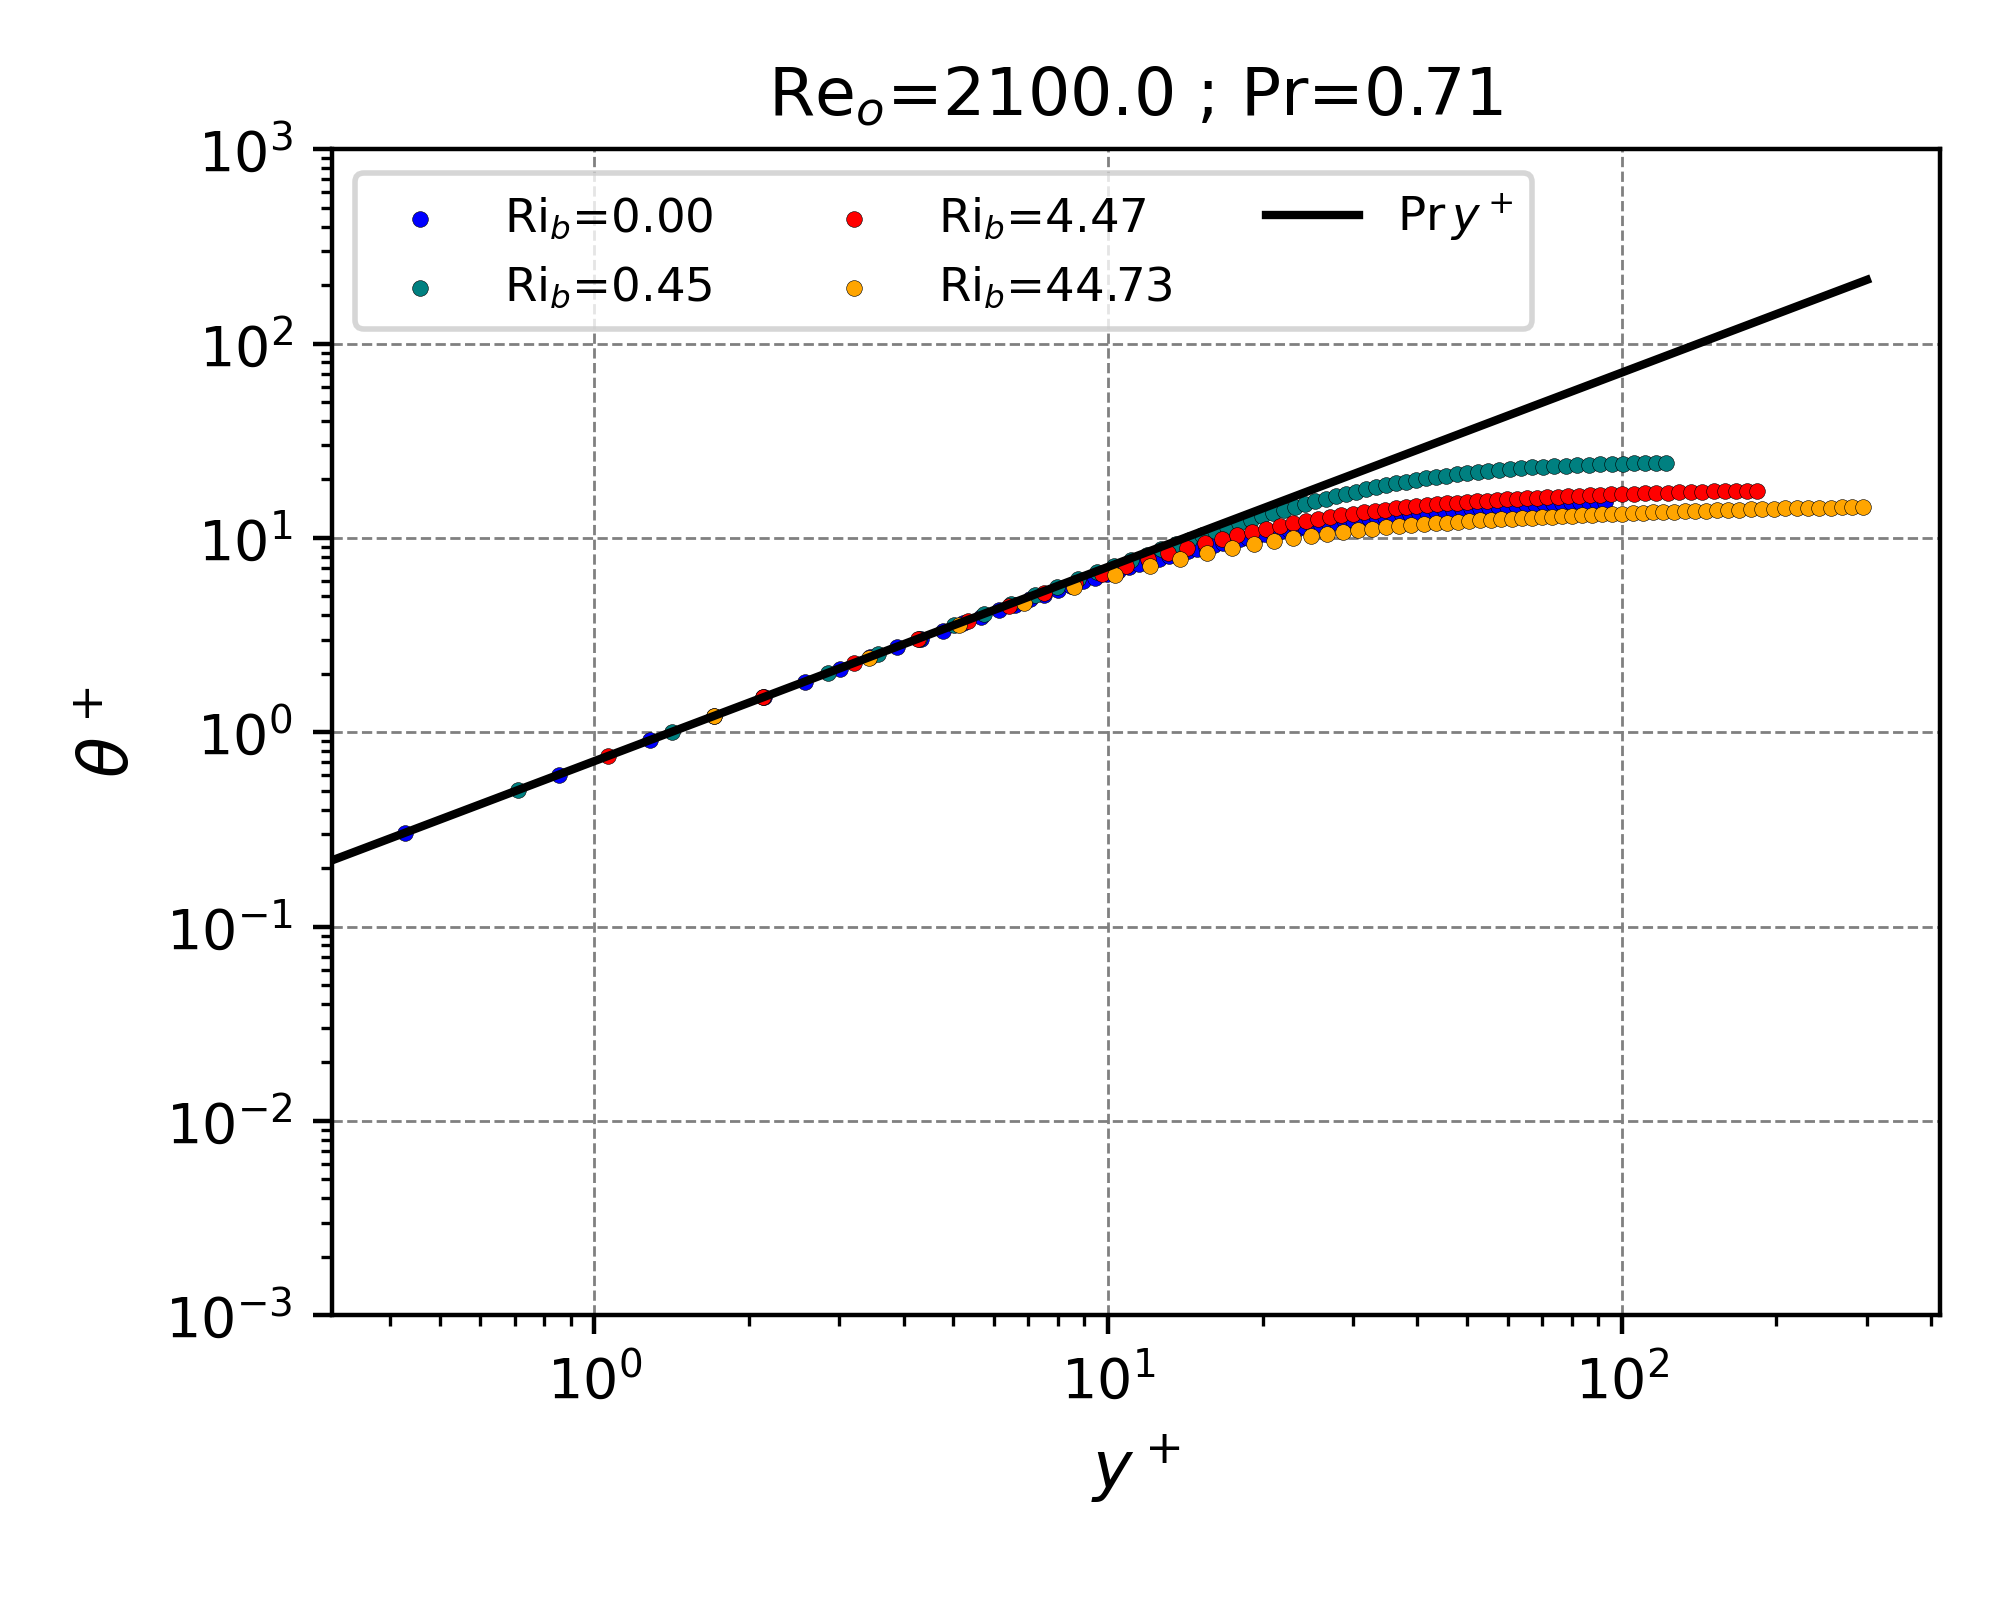
\includegraphics[width=0.45\textwidth]{figures/cap5/Re2100-Pr071/phi_mean_plus_log_profile.png}}
  \subfloat[]{
    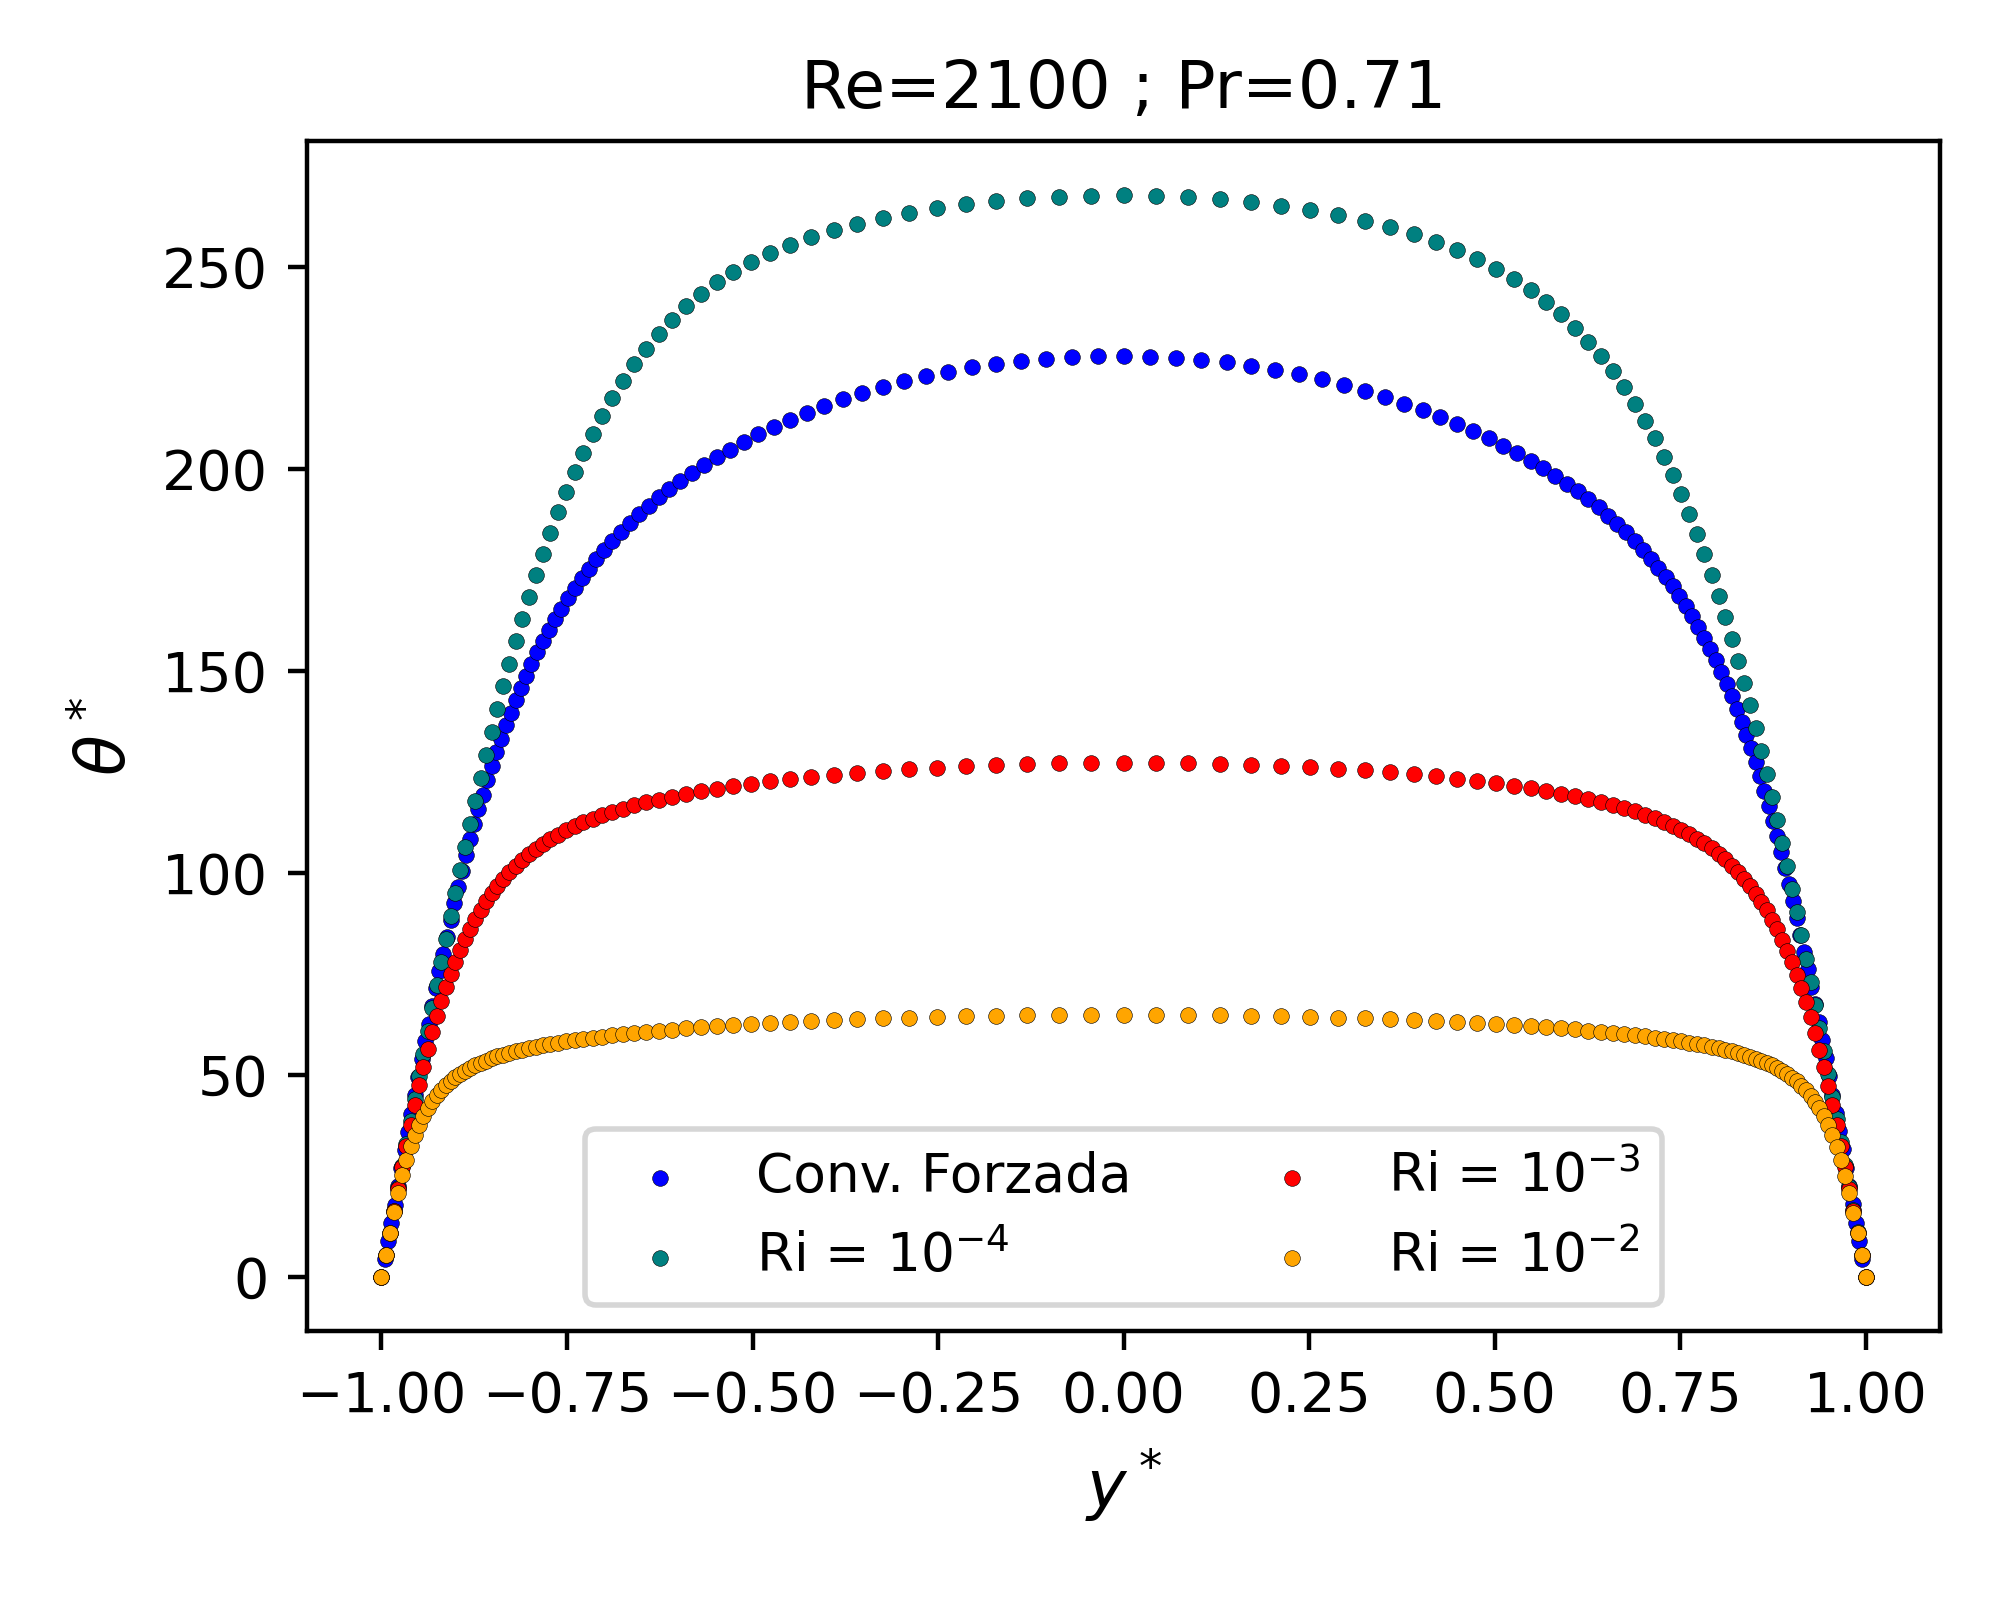
\includegraphics[width=0.45\textwidth]{figures/cap5/Re2100-Pr071/phi_mean_profile.png}}
  \caption{}
  \label{fig:phi-Re2100-Pr071}
\end{figure}

\begin{figure}[H]
  \centering
  \subfloat[]{
    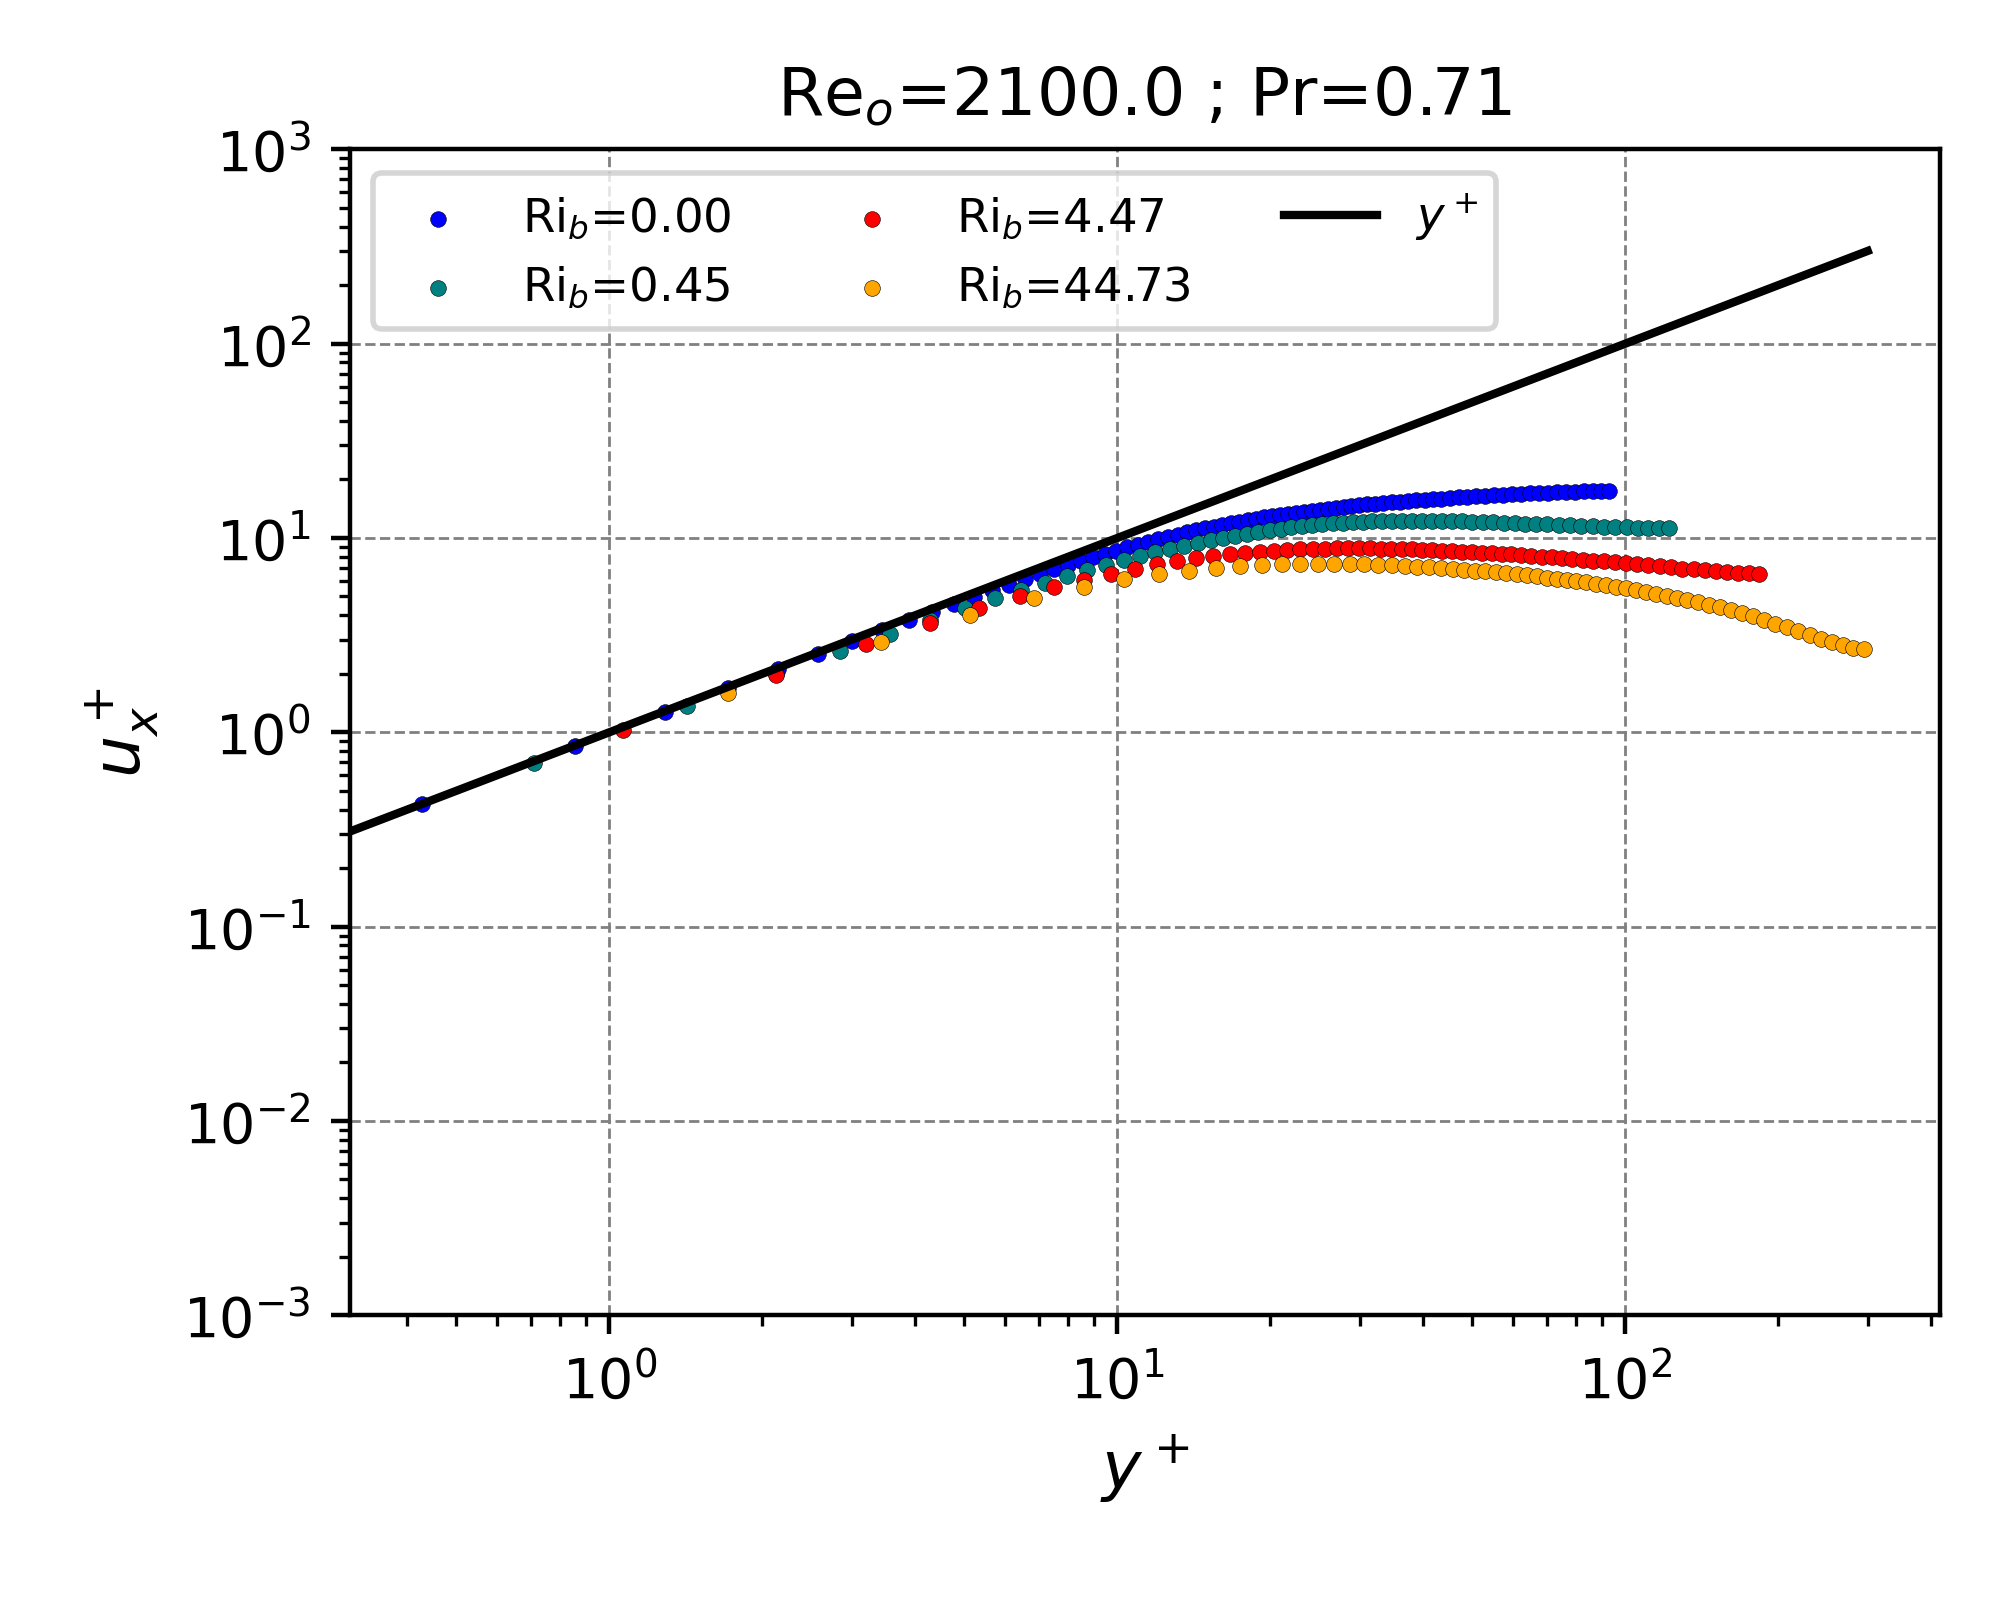
\includegraphics[width=0.45\textwidth]{figures/cap5/Re2100-Pr071/ux_mean_plus_log_profile.png}}
  \subfloat[]{
    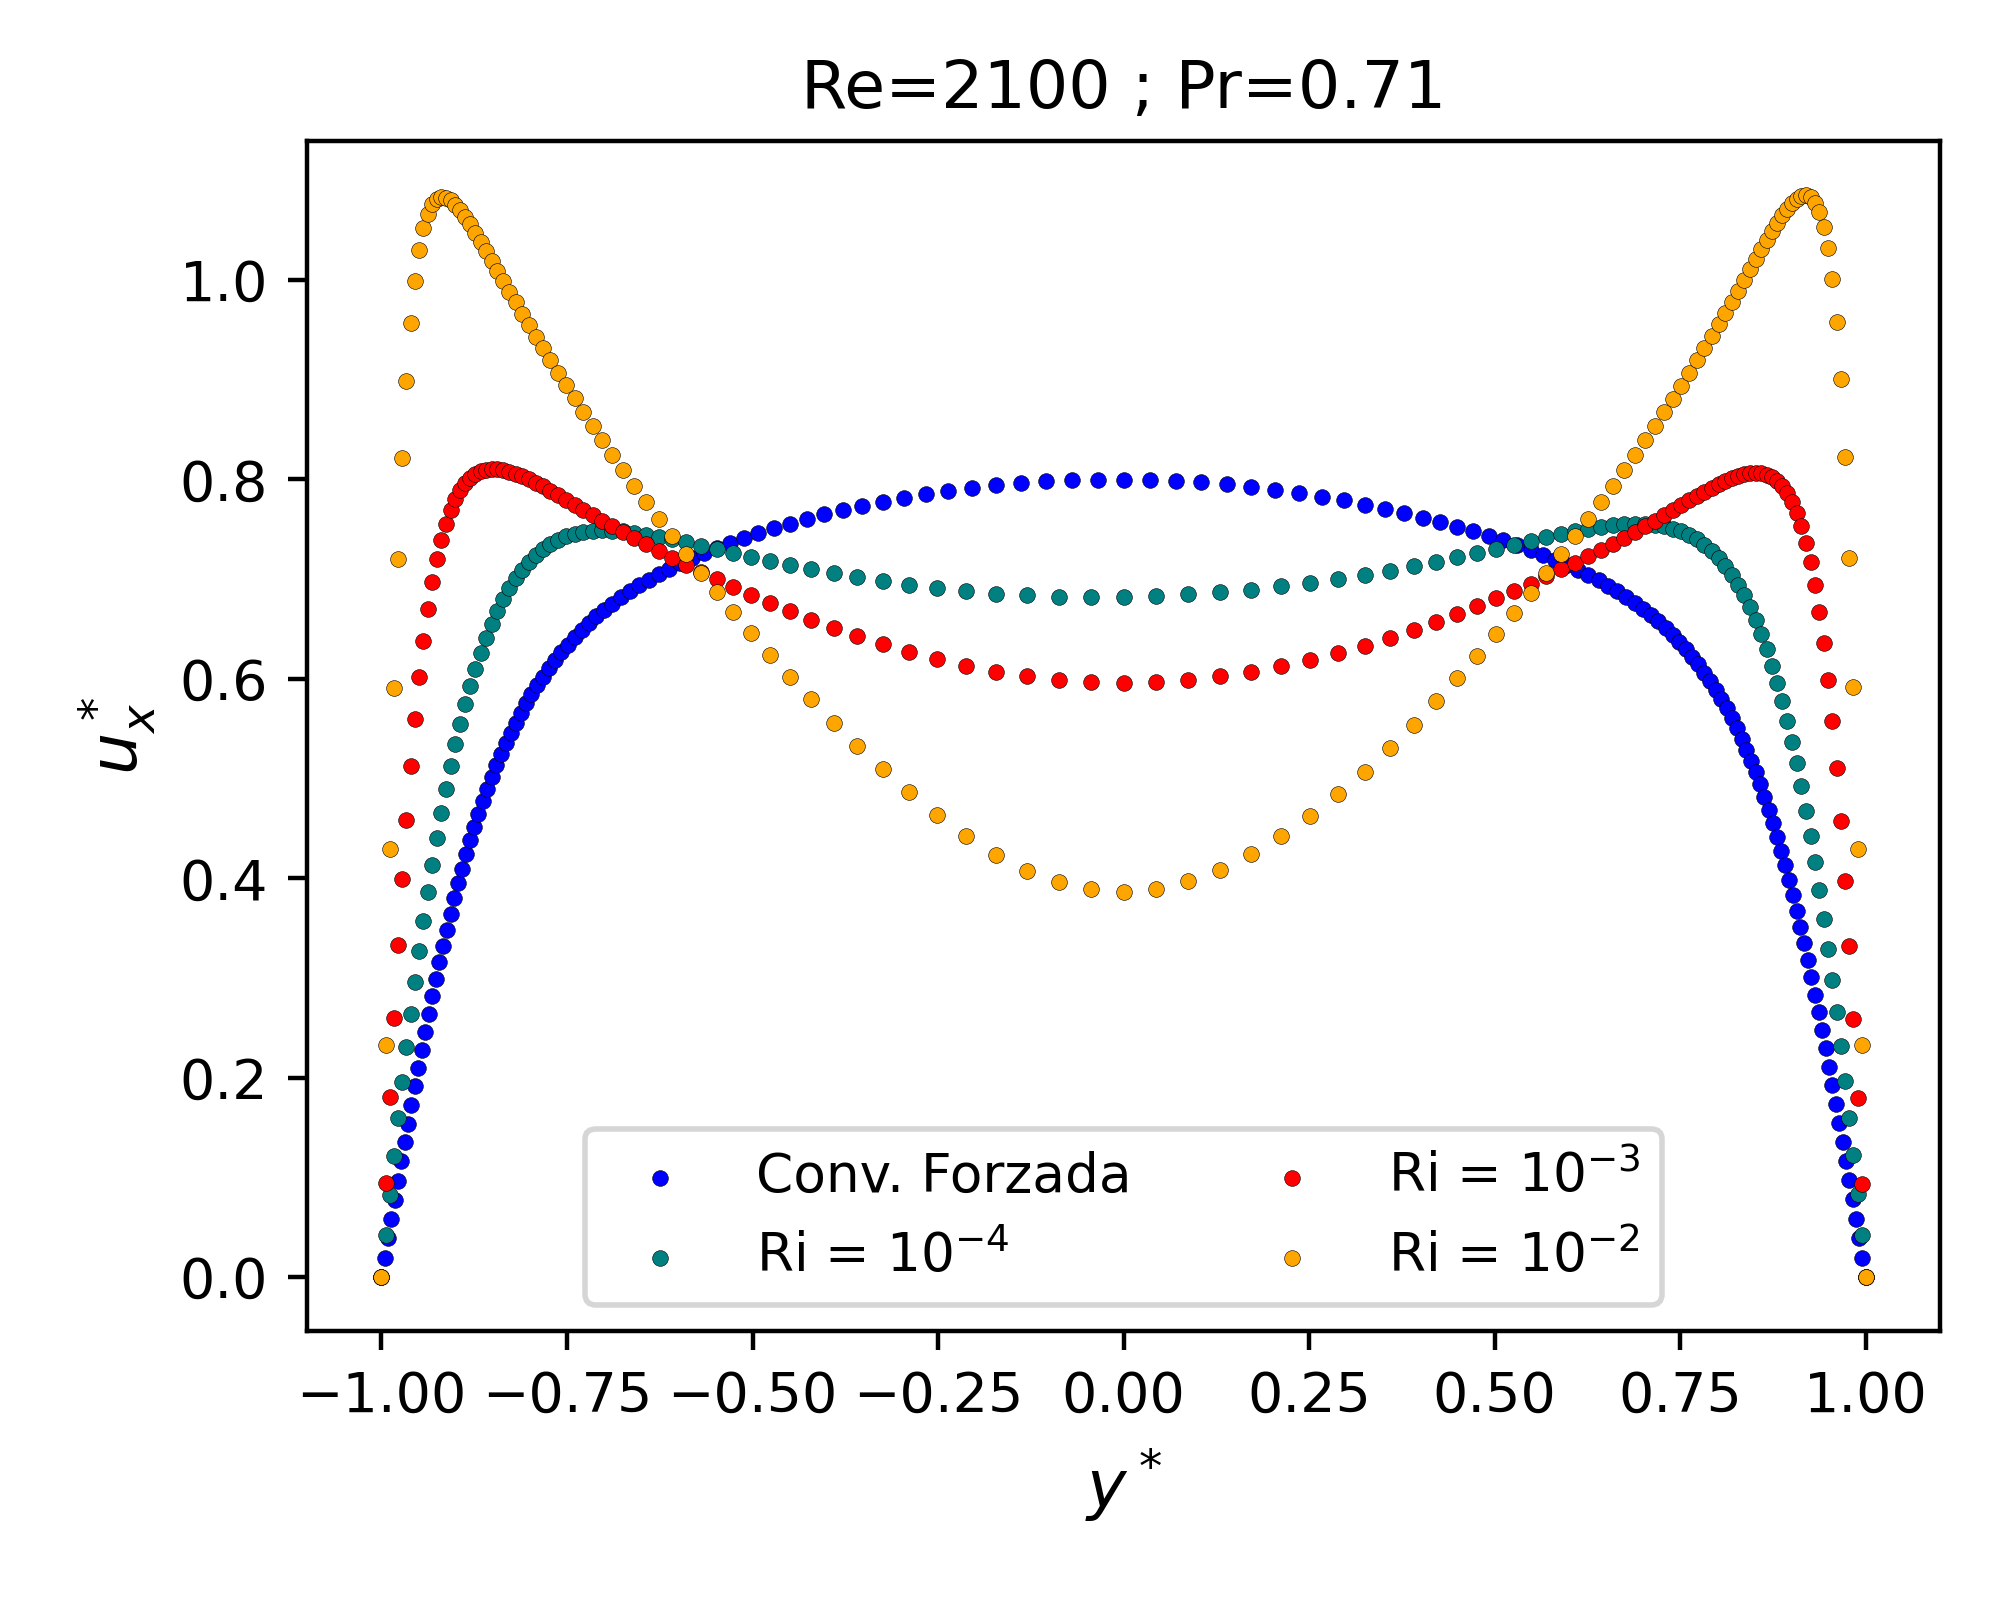
\includegraphics[width=0.45\textwidth]{figures/cap5/Re2100-Pr071/ux_mean_profile.png}}
  \caption{}
  \label{fig:ux-Re2100-Pr071}
\end{figure}

%% ==============================================================
%%  Re = 2100, Pr = 0.071
%% ==============================================================

\section{$\text{Re}=2100$ y $\text{Pr}=0.071$}

\begin{figure}[H]
  \centering
  \subfloat[]{
    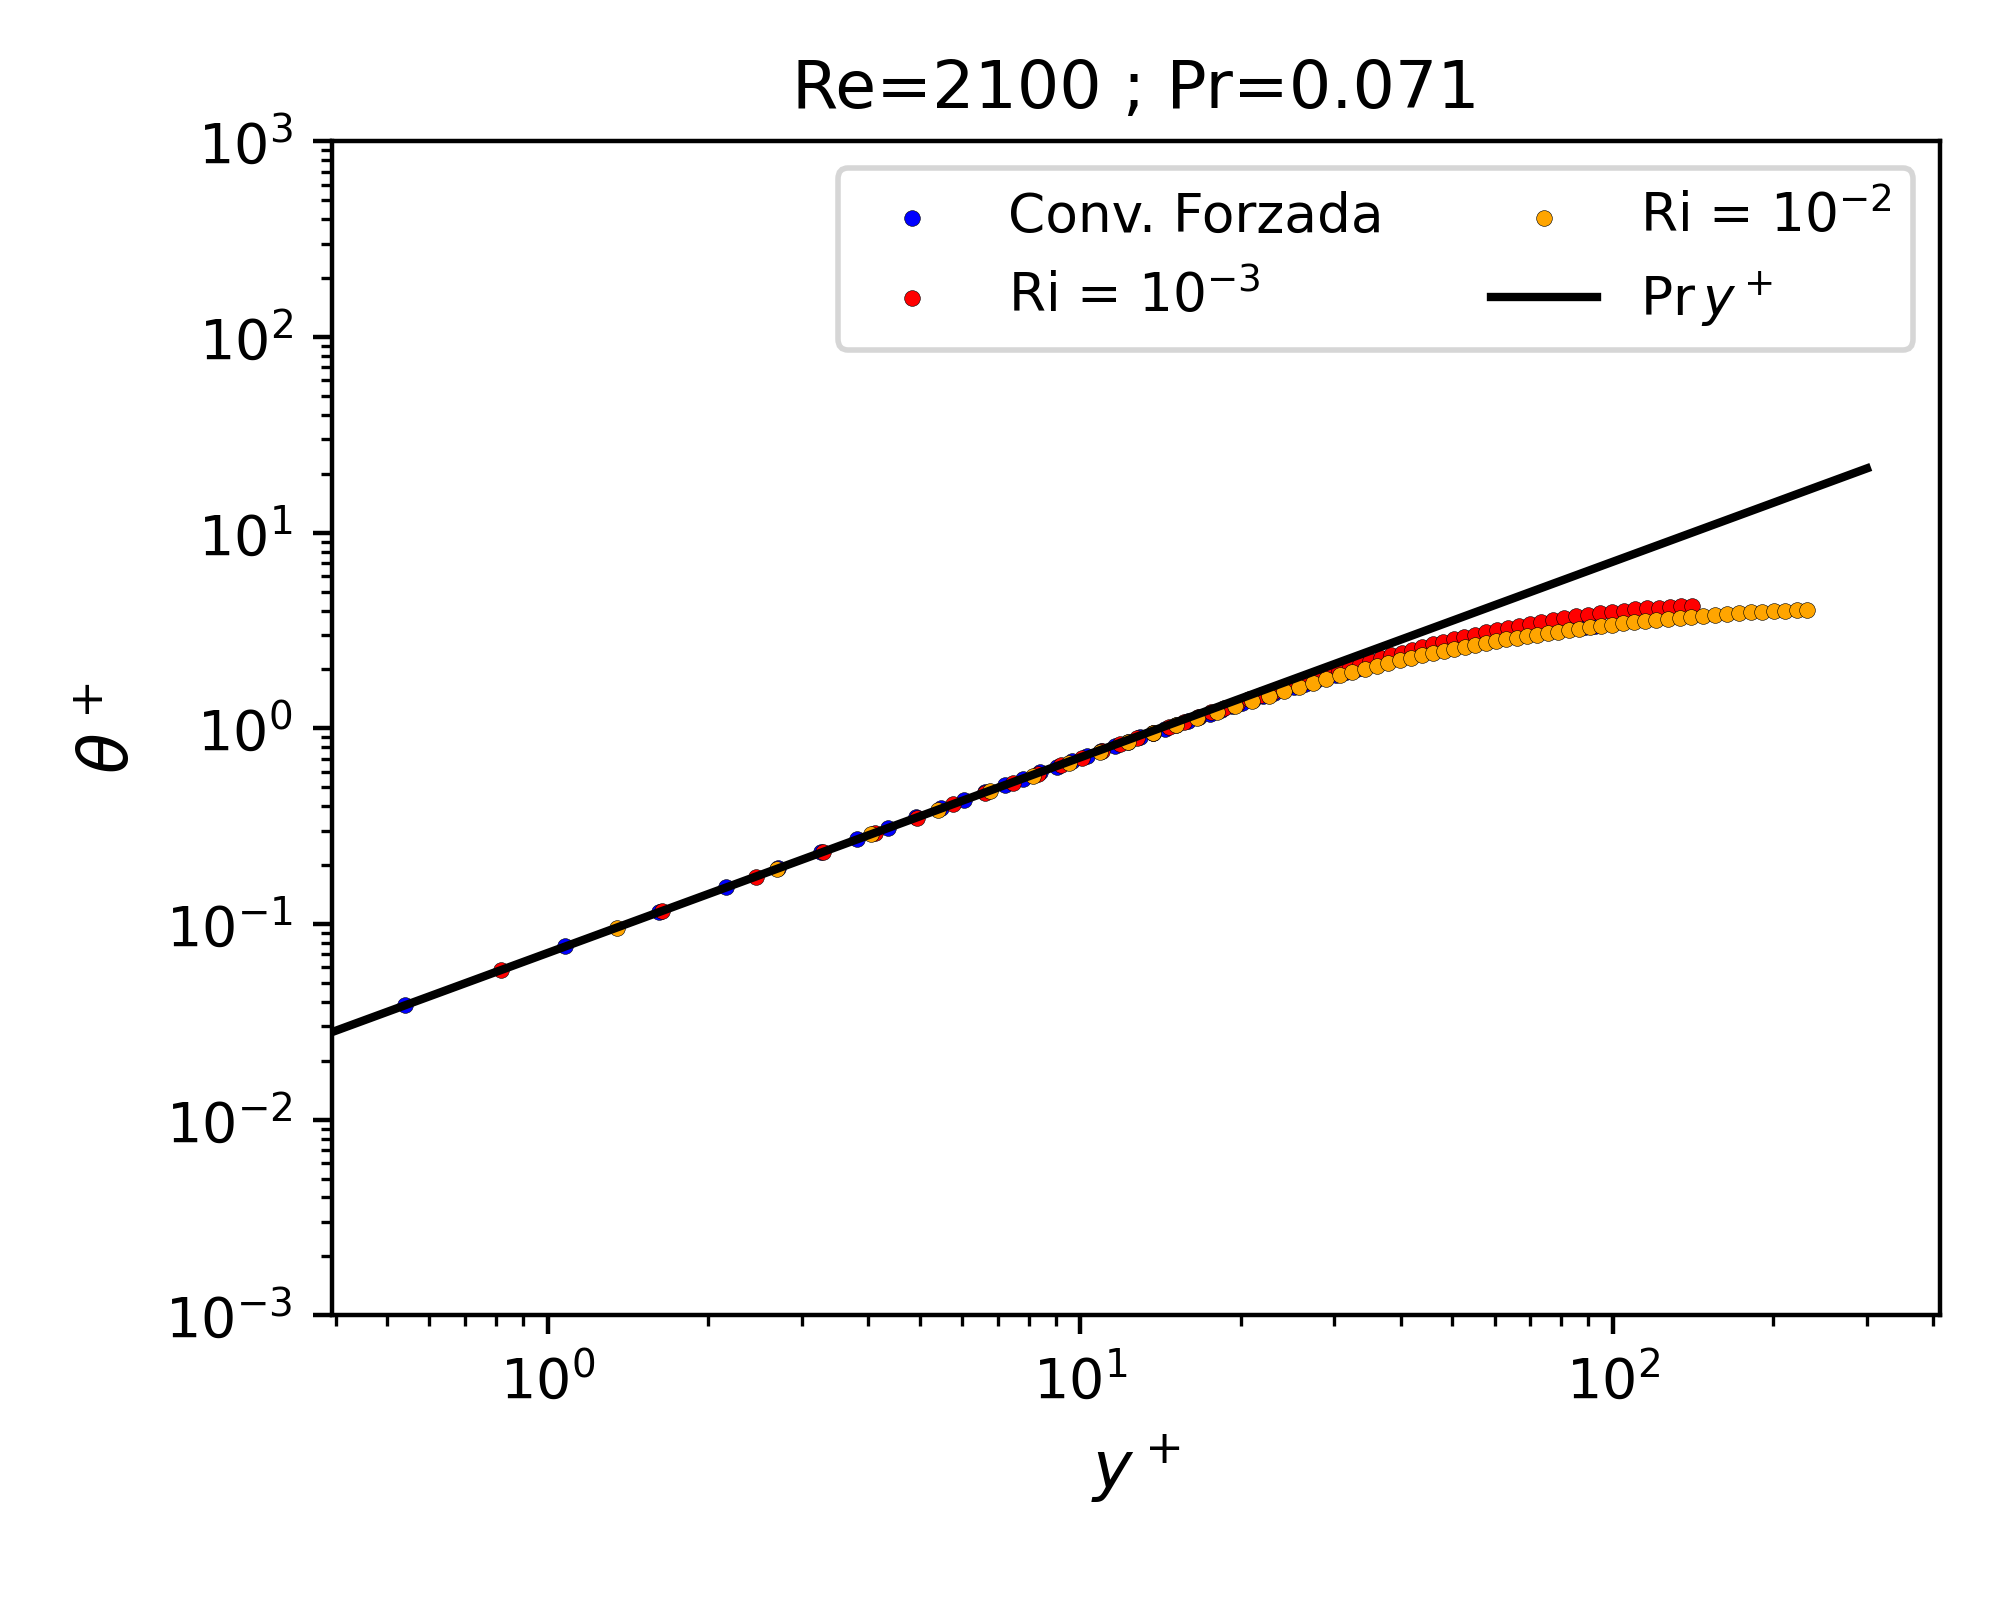
\includegraphics[width=0.45\textwidth]{figures/cap5/Re2100-Pr0071/phi_mean_plus_log_profile.png}}
  \subfloat[]{
    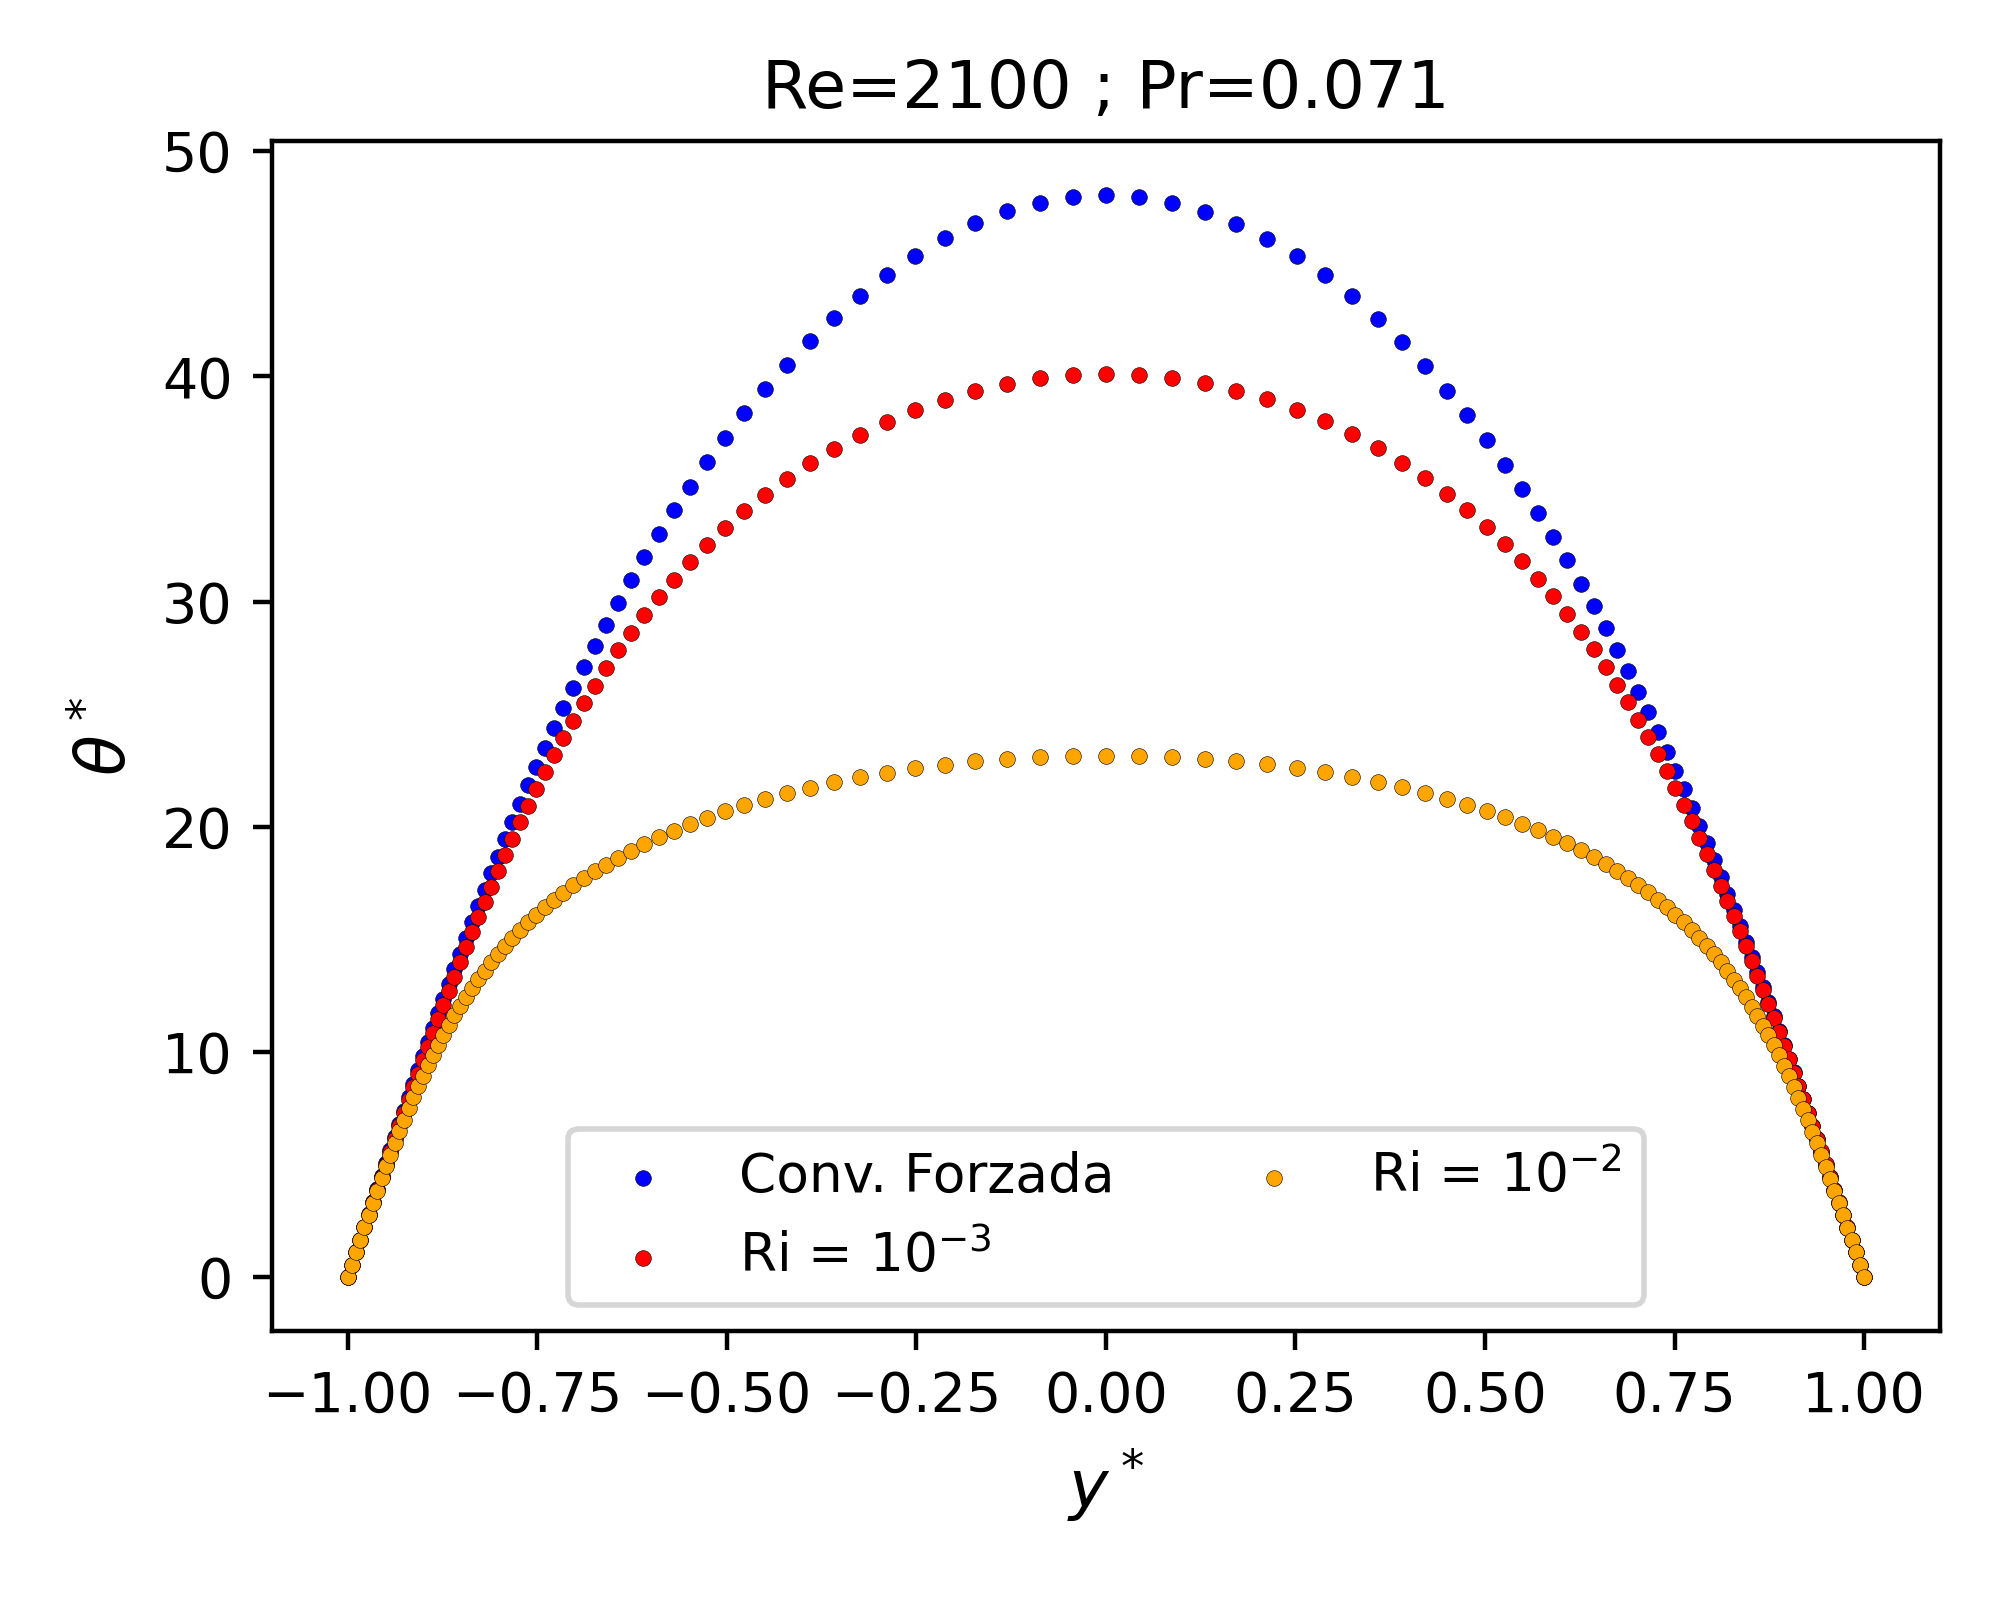
\includegraphics[width=0.45\textwidth]{figures/cap5/Re2100-Pr0071/phi_mean_profile.png}}
  \caption{}
  \label{fig:phi-Re2100-Pr0071}
\end{figure}

\begin{figure}[H]
  \centering
  \subfloat[]{
    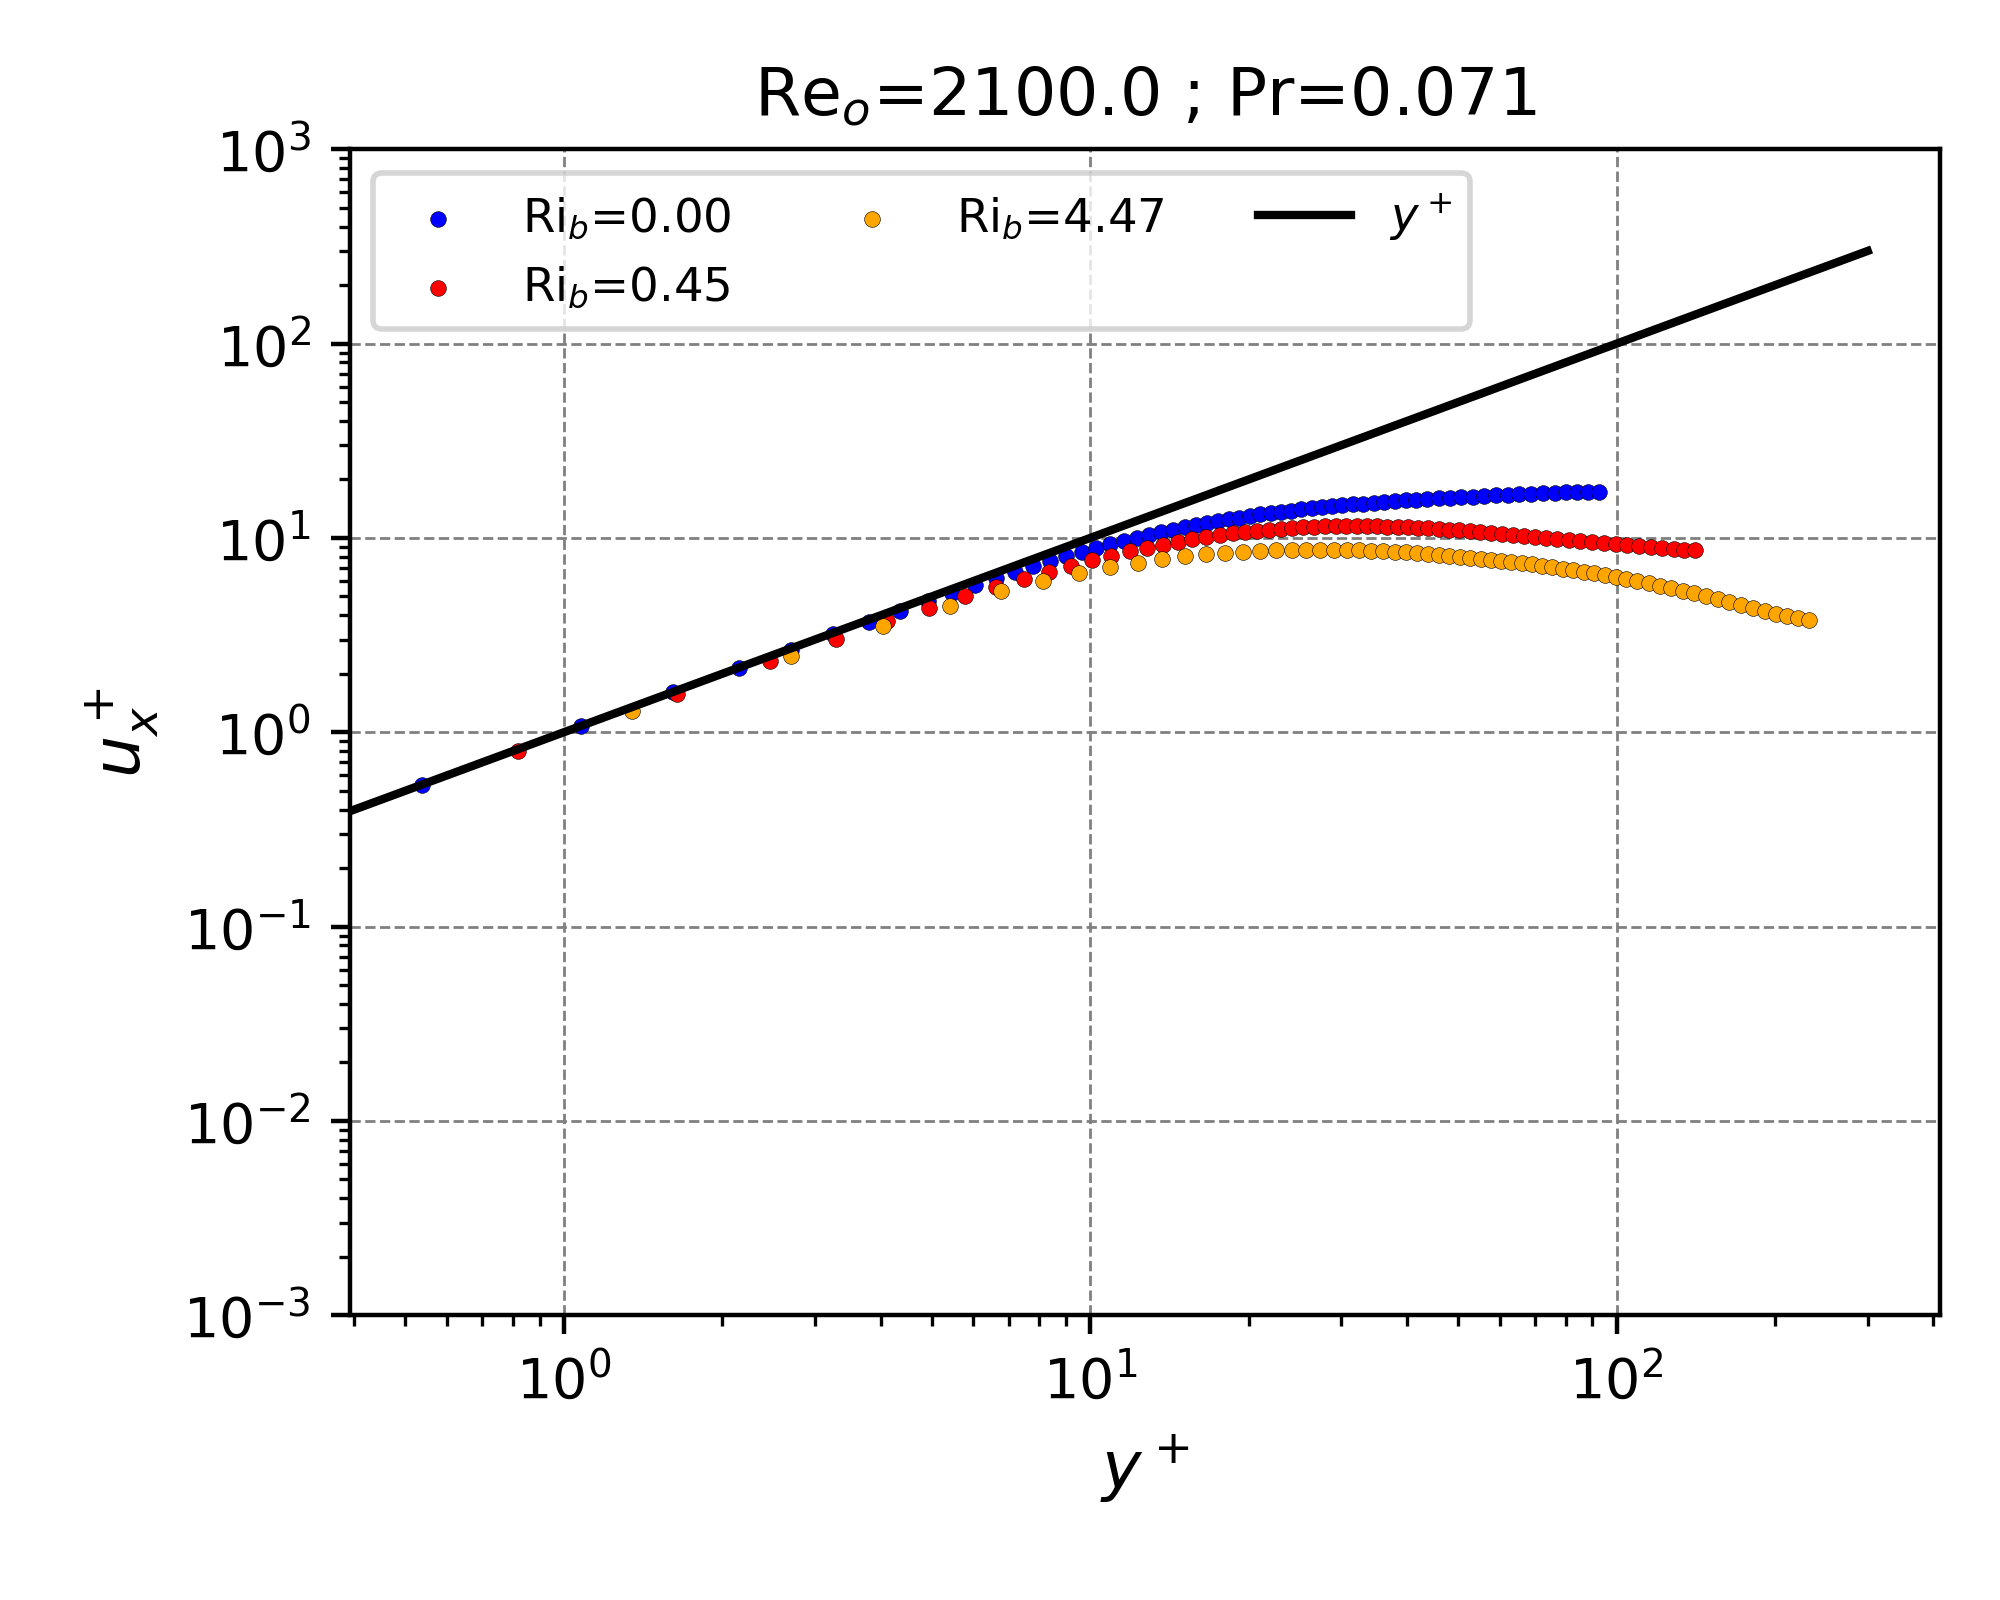
\includegraphics[width=0.45\textwidth]{figures/cap5/Re2100-Pr0071/ux_mean_plus_log_profile.png}}
  \subfloat[]{
    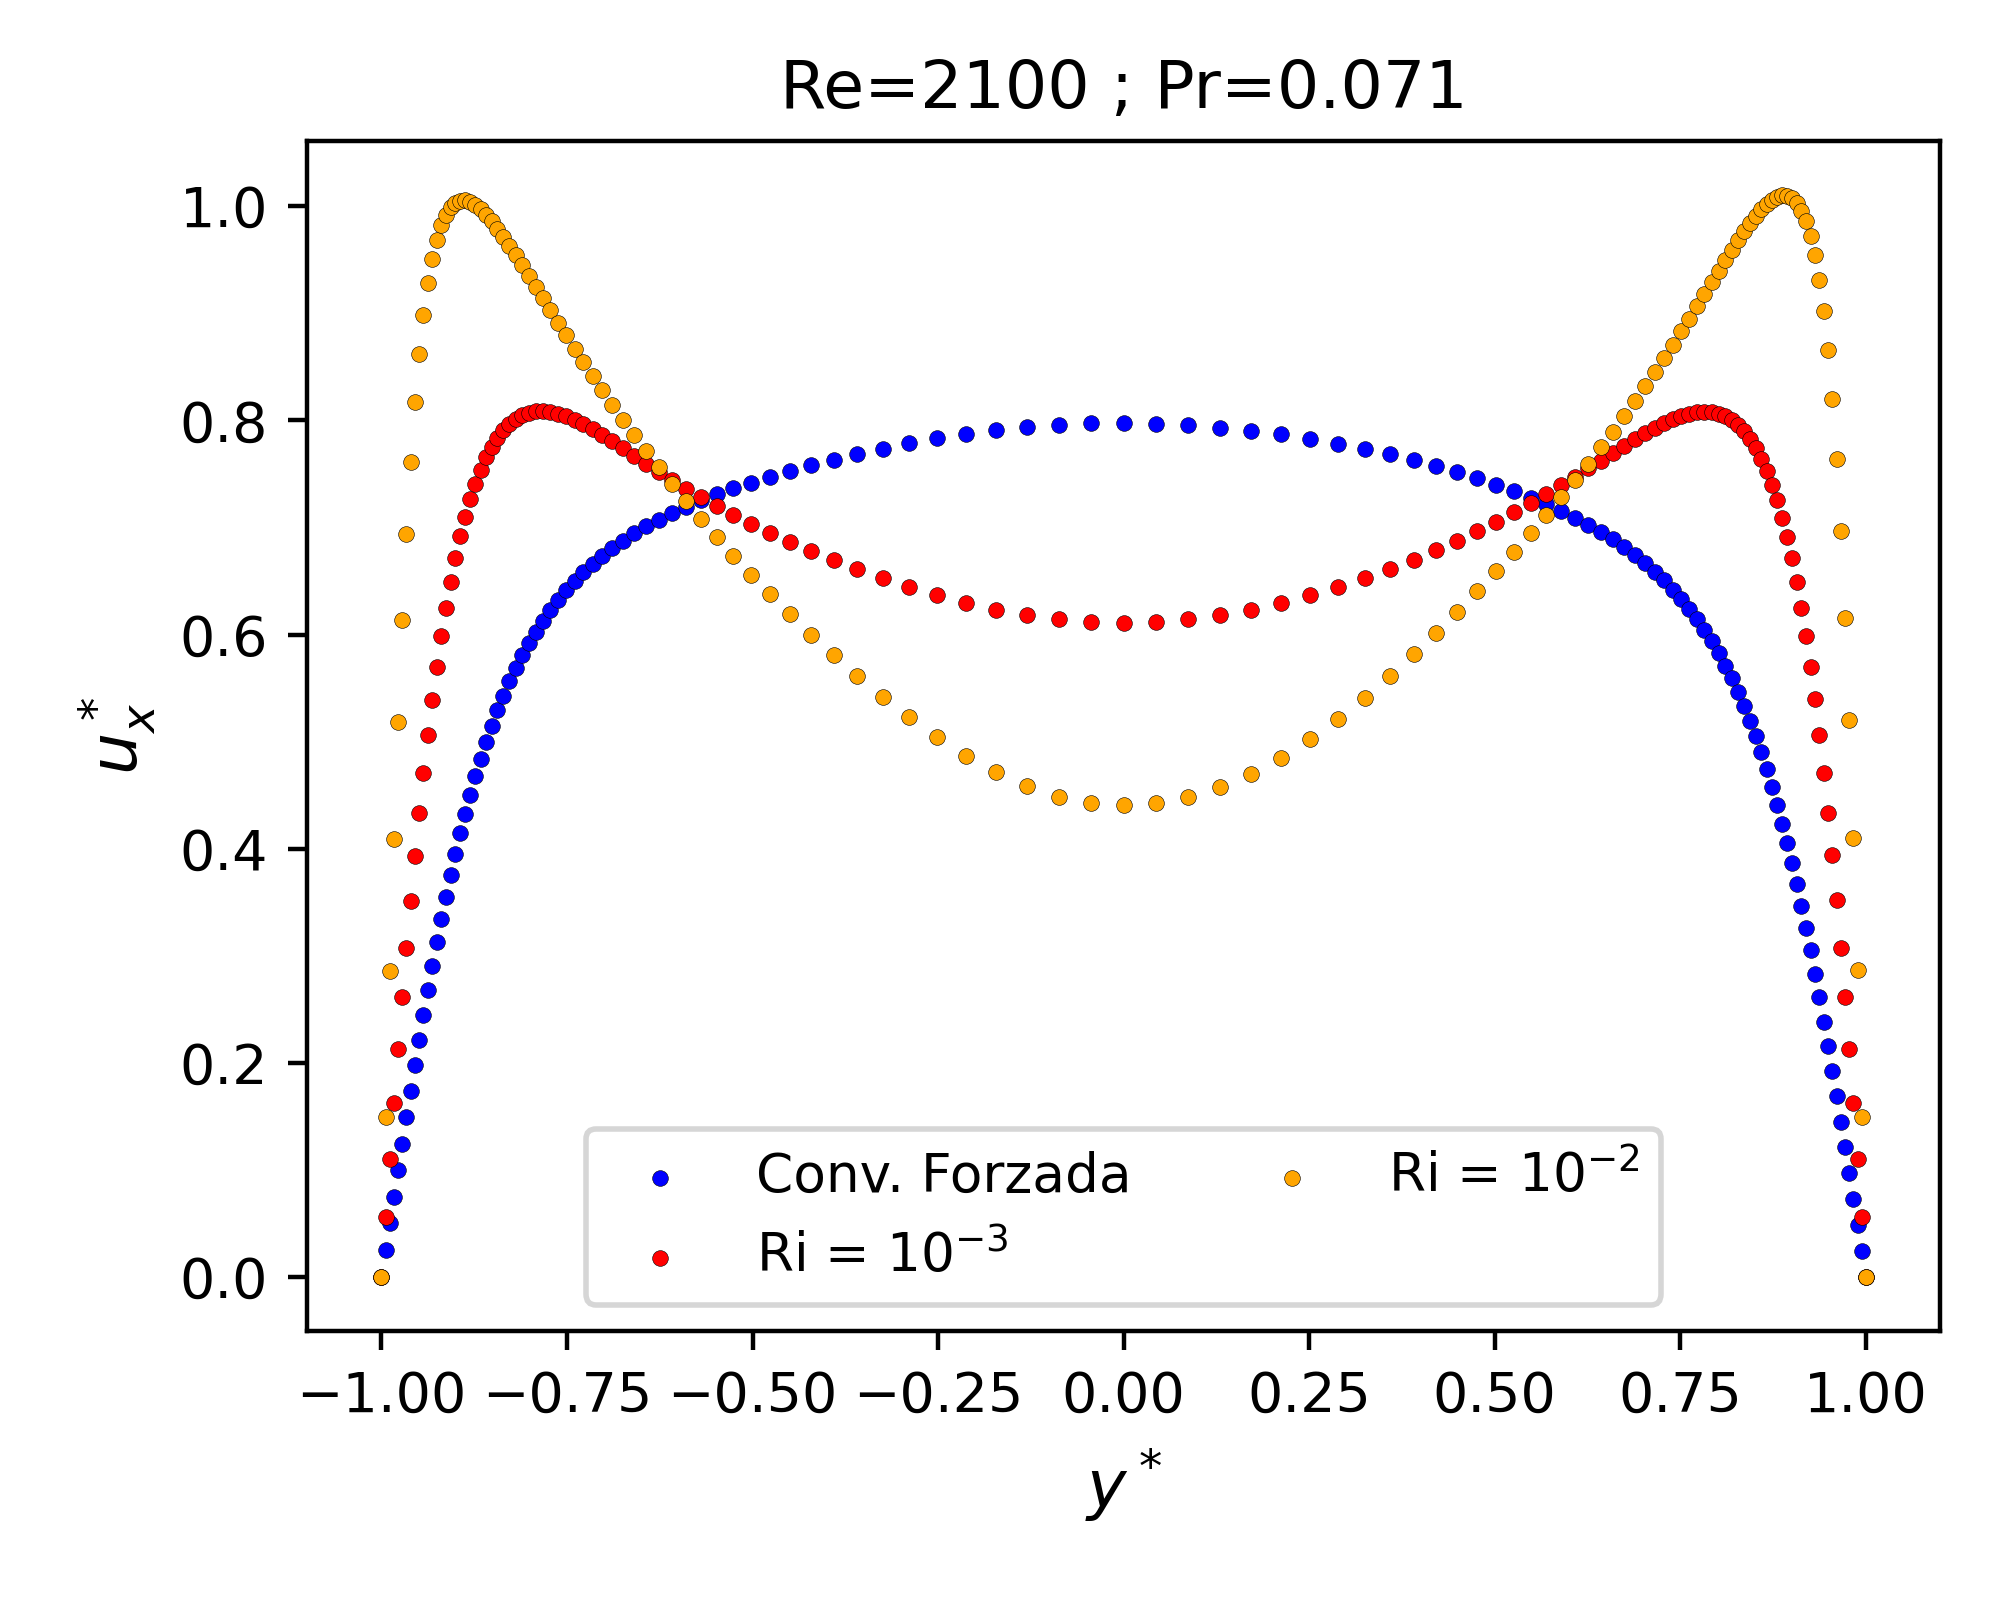
\includegraphics[width=0.45\textwidth]{figures/cap5/Re2100-Pr0071/ux_mean_profile.png}}
  \caption{}
  \label{fig:ux-Re2100-Pr0071}
\end{figure}

%% ==============================================================
%%  Re = 3150, Pr = 0.71
%% ==============================================================

\section{$\text{Re}=3150$ y $\text{Pr}=0.71$}

\begin{figure}[H]
  \centering
  \subfloat[]{
    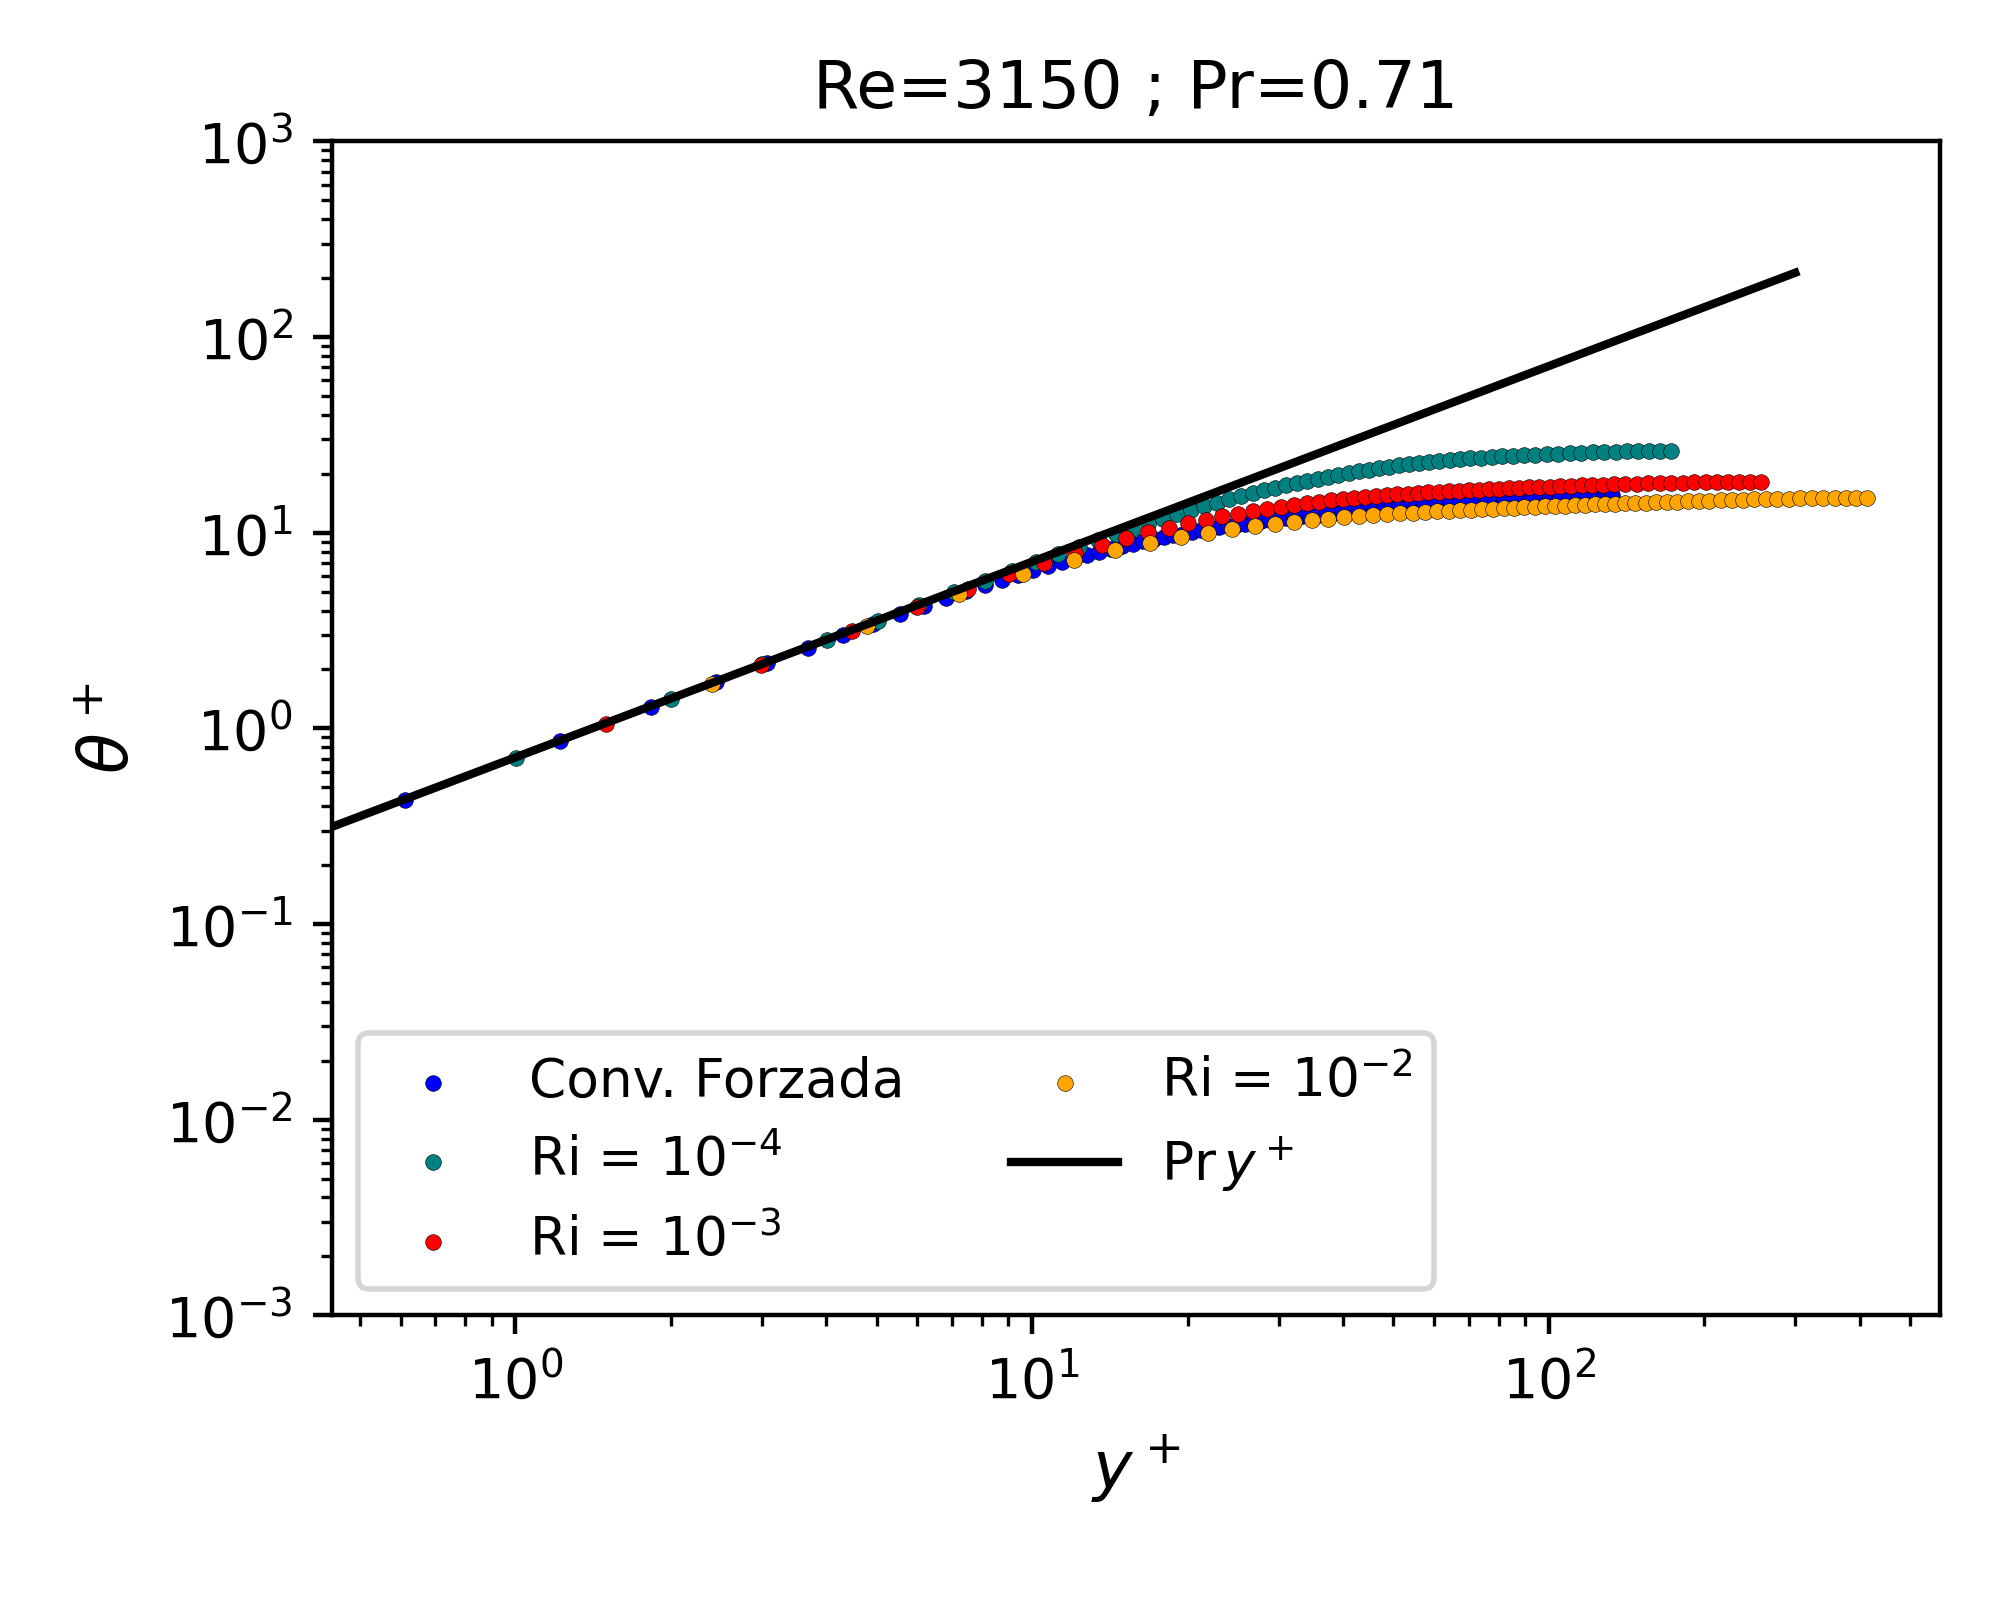
\includegraphics[width=0.45\textwidth]{figures/cap5/Re3150-Pr071/phi_mean_plus_log_profile.png}}
  \subfloat[]{
    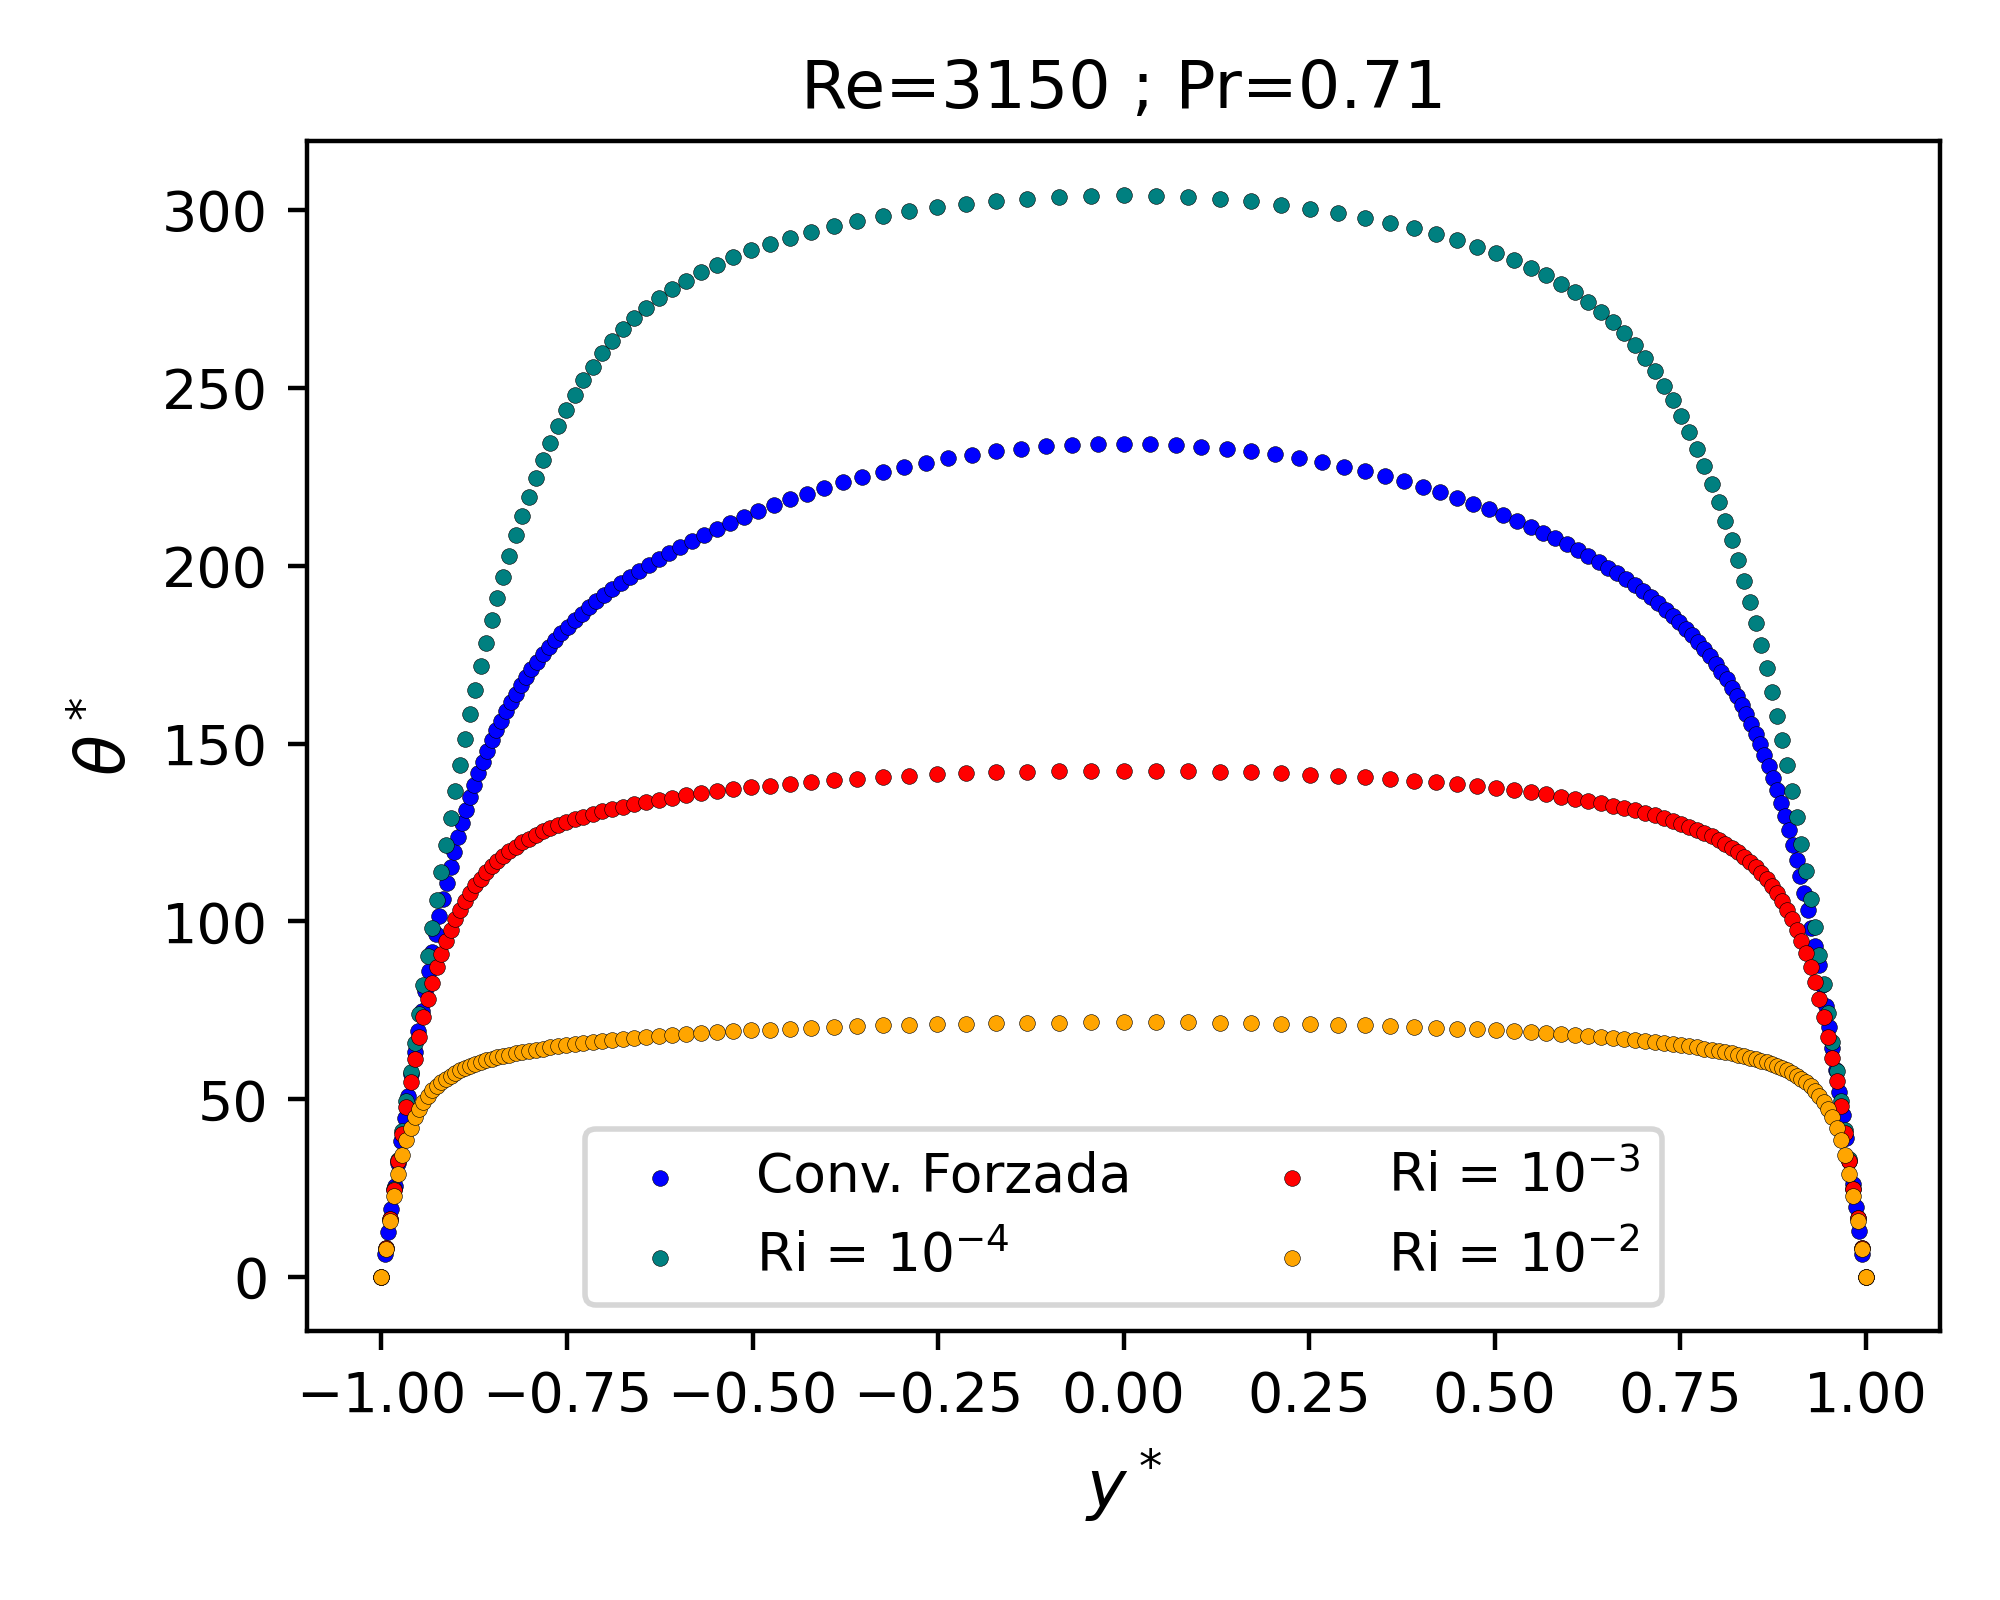
\includegraphics[width=0.45\textwidth]{figures/cap5/Re3150-Pr071/phi_mean_profile.png}}
  \caption{}
  \label{fig:phi-Re3150-Pr071}
\end{figure}

\begin{figure}[H]
  \centering
  \subfloat[]{
    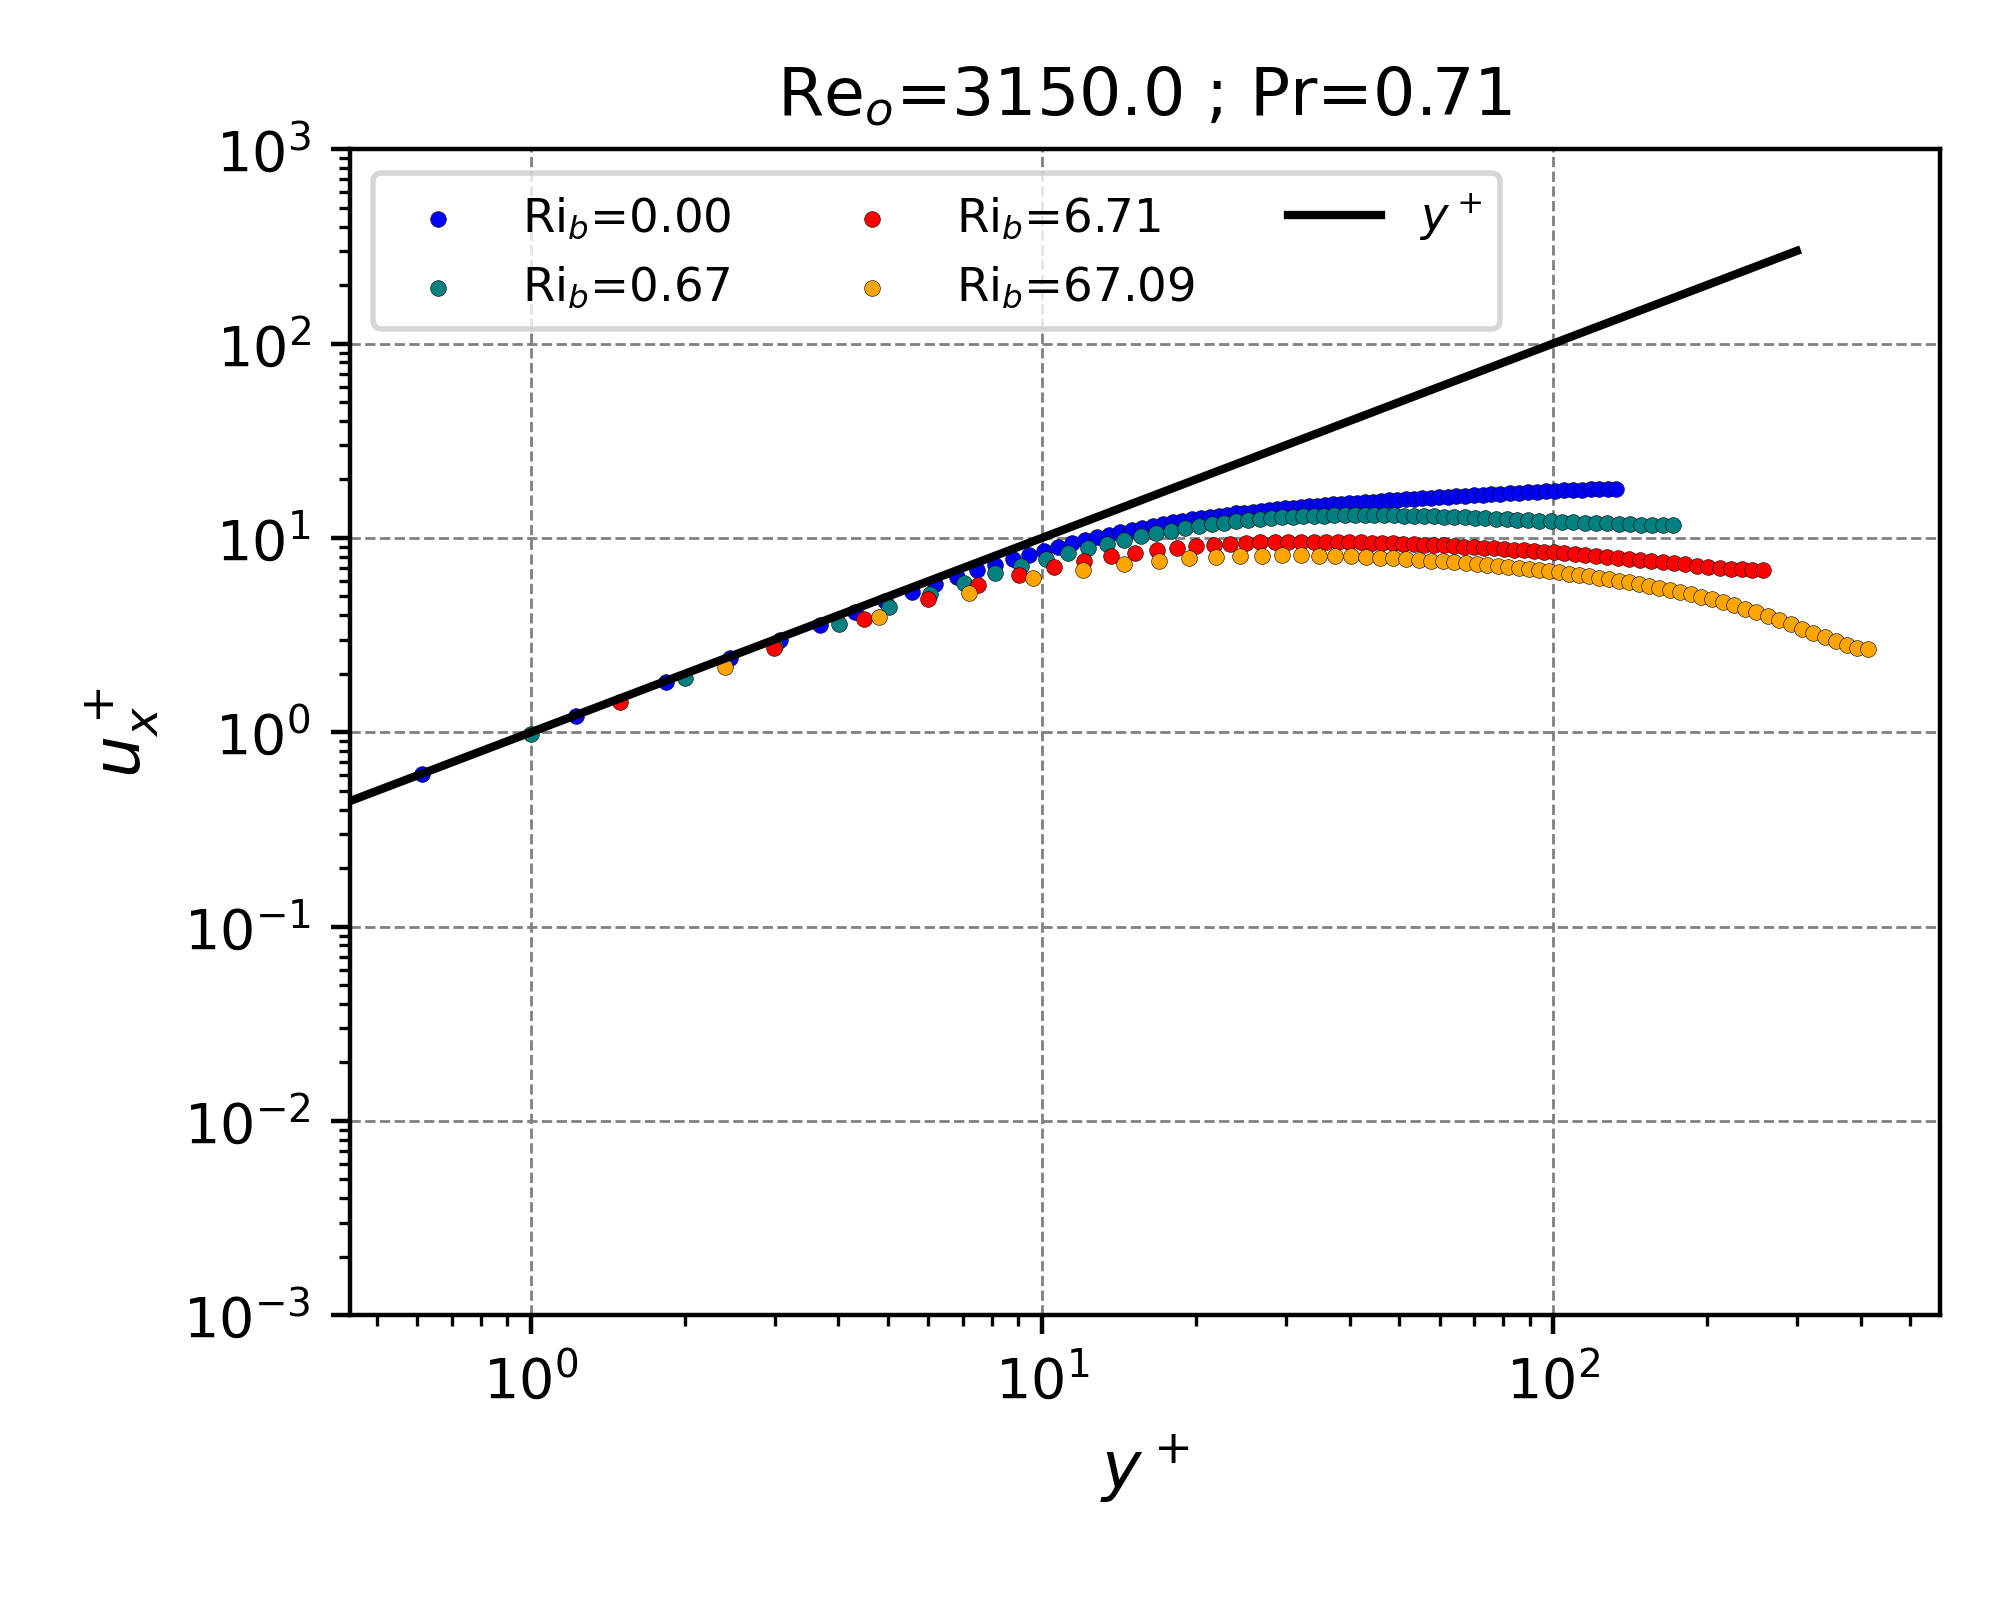
\includegraphics[width=0.45\textwidth]{figures/cap5/Re3150-Pr071/ux_mean_plus_log_profile.png}}
  \subfloat[]{
    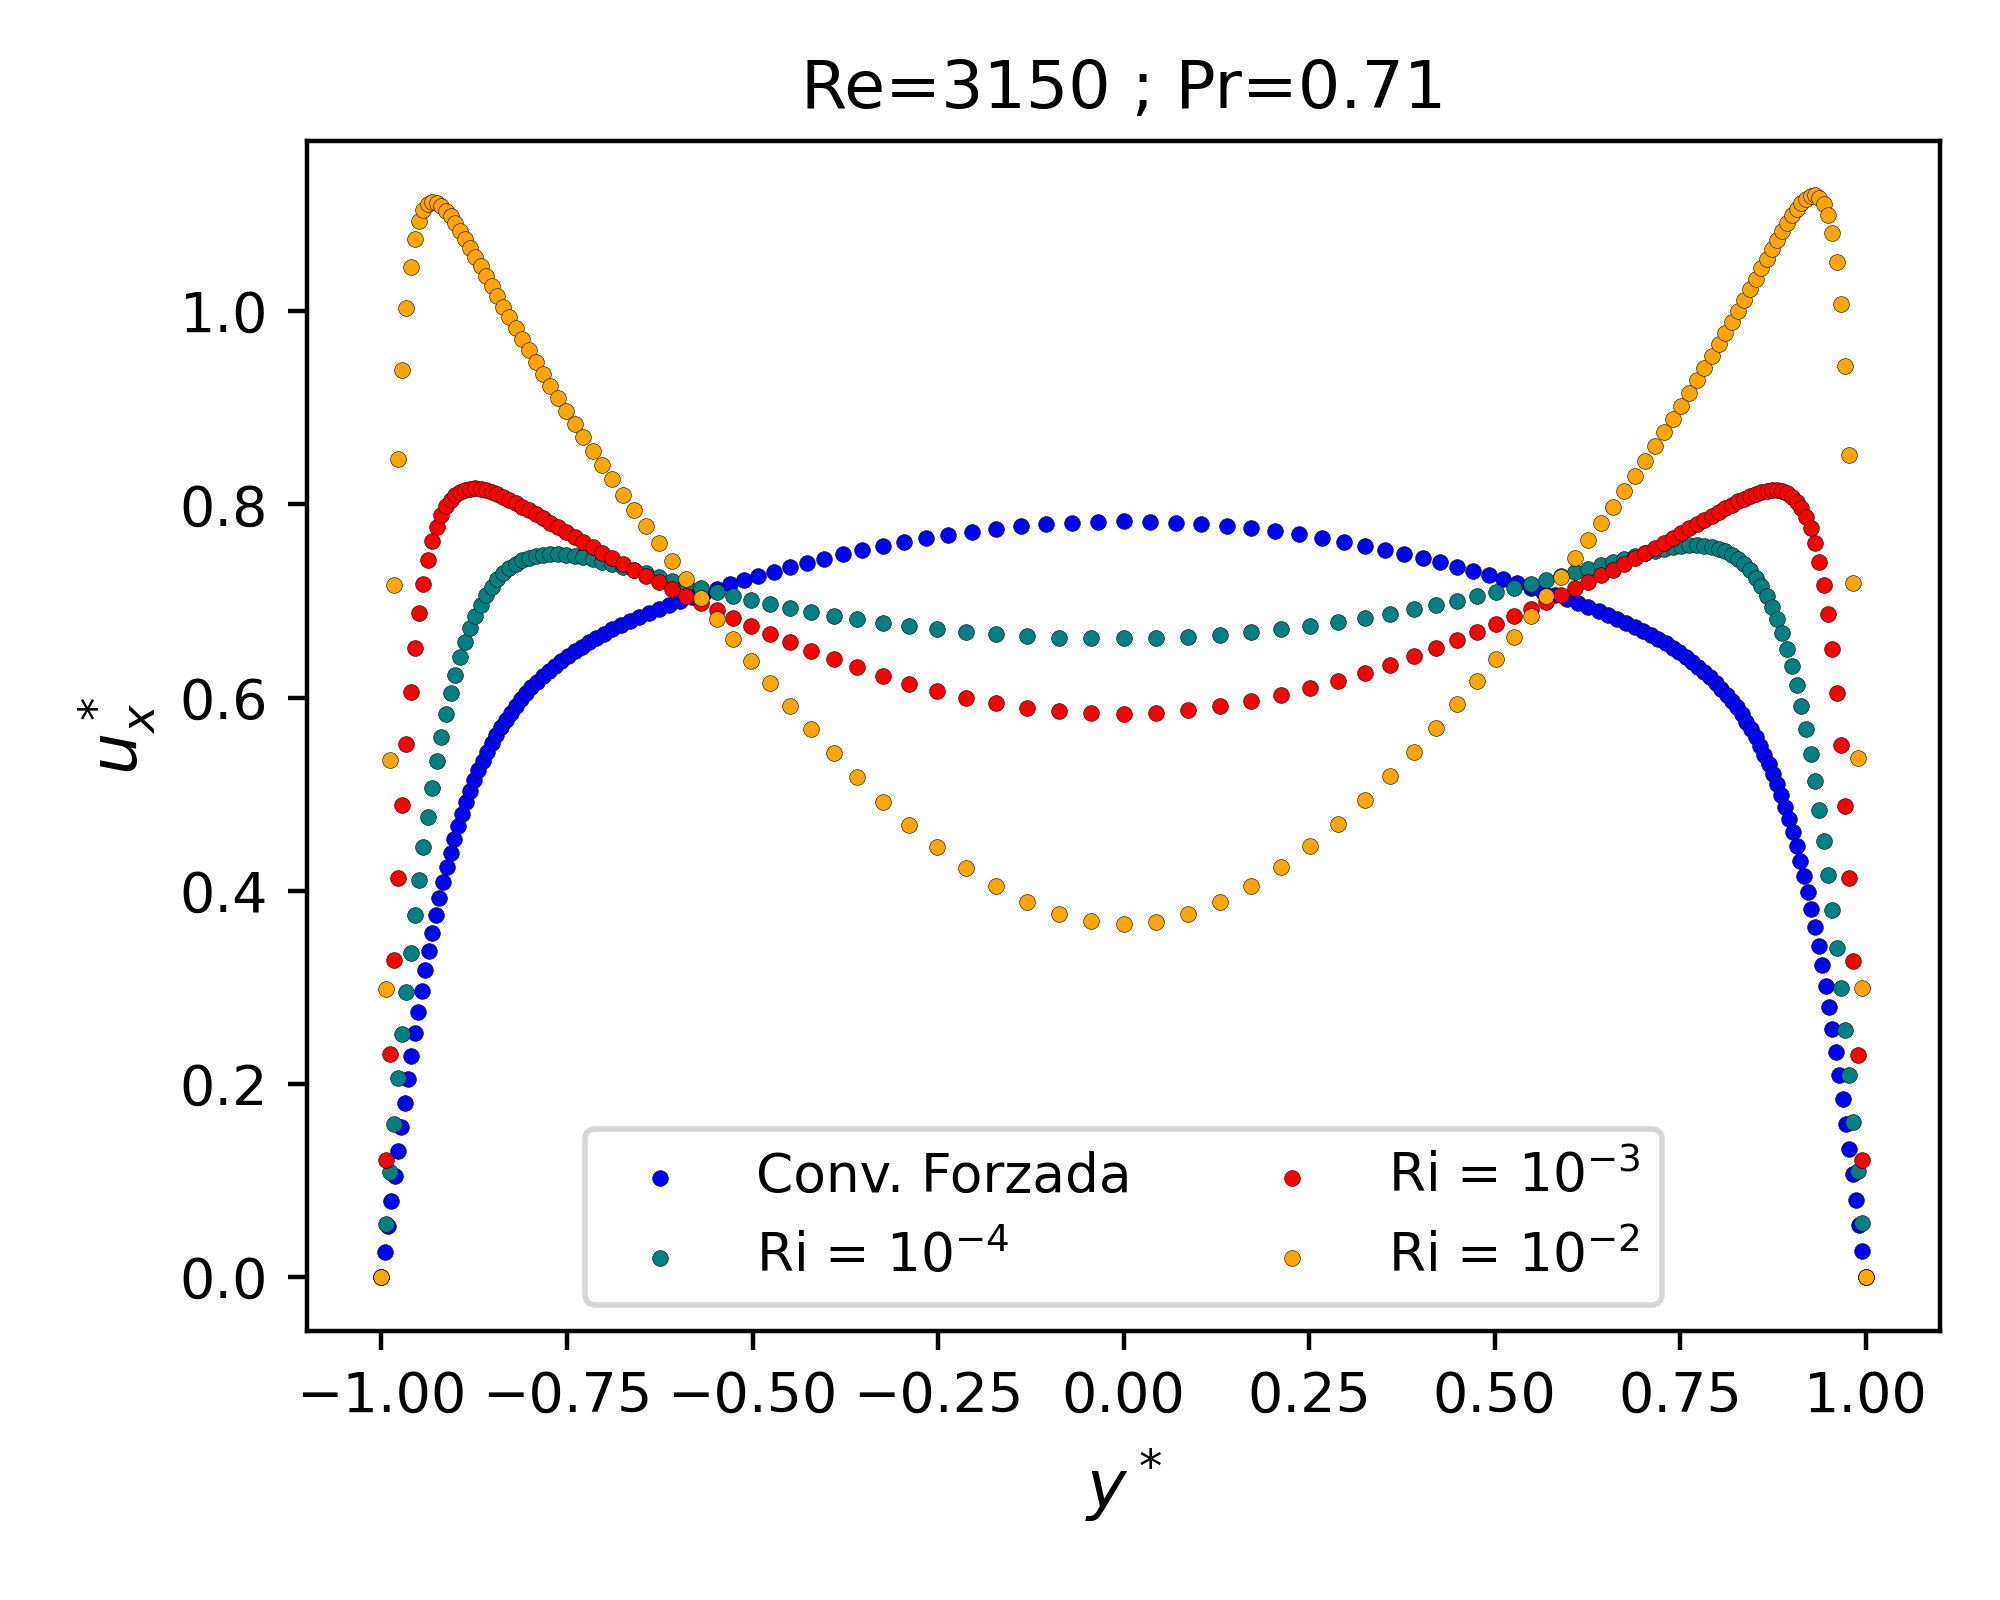
\includegraphics[width=0.45\textwidth]{figures/cap5/Re3150-Pr071/ux_mean_profile.png}}
  \caption{}
  \label{fig:ux-Re3150-Pr071}
\end{figure}

%% ==============================================================
%%  Re = 3150, Pr = 0.071
%% ==============================================================

\section{$\text{Re}=3150$ y $\text{Pr}=0.071$}

\begin{figure}[H]
  \centering
  \subfloat[]{
    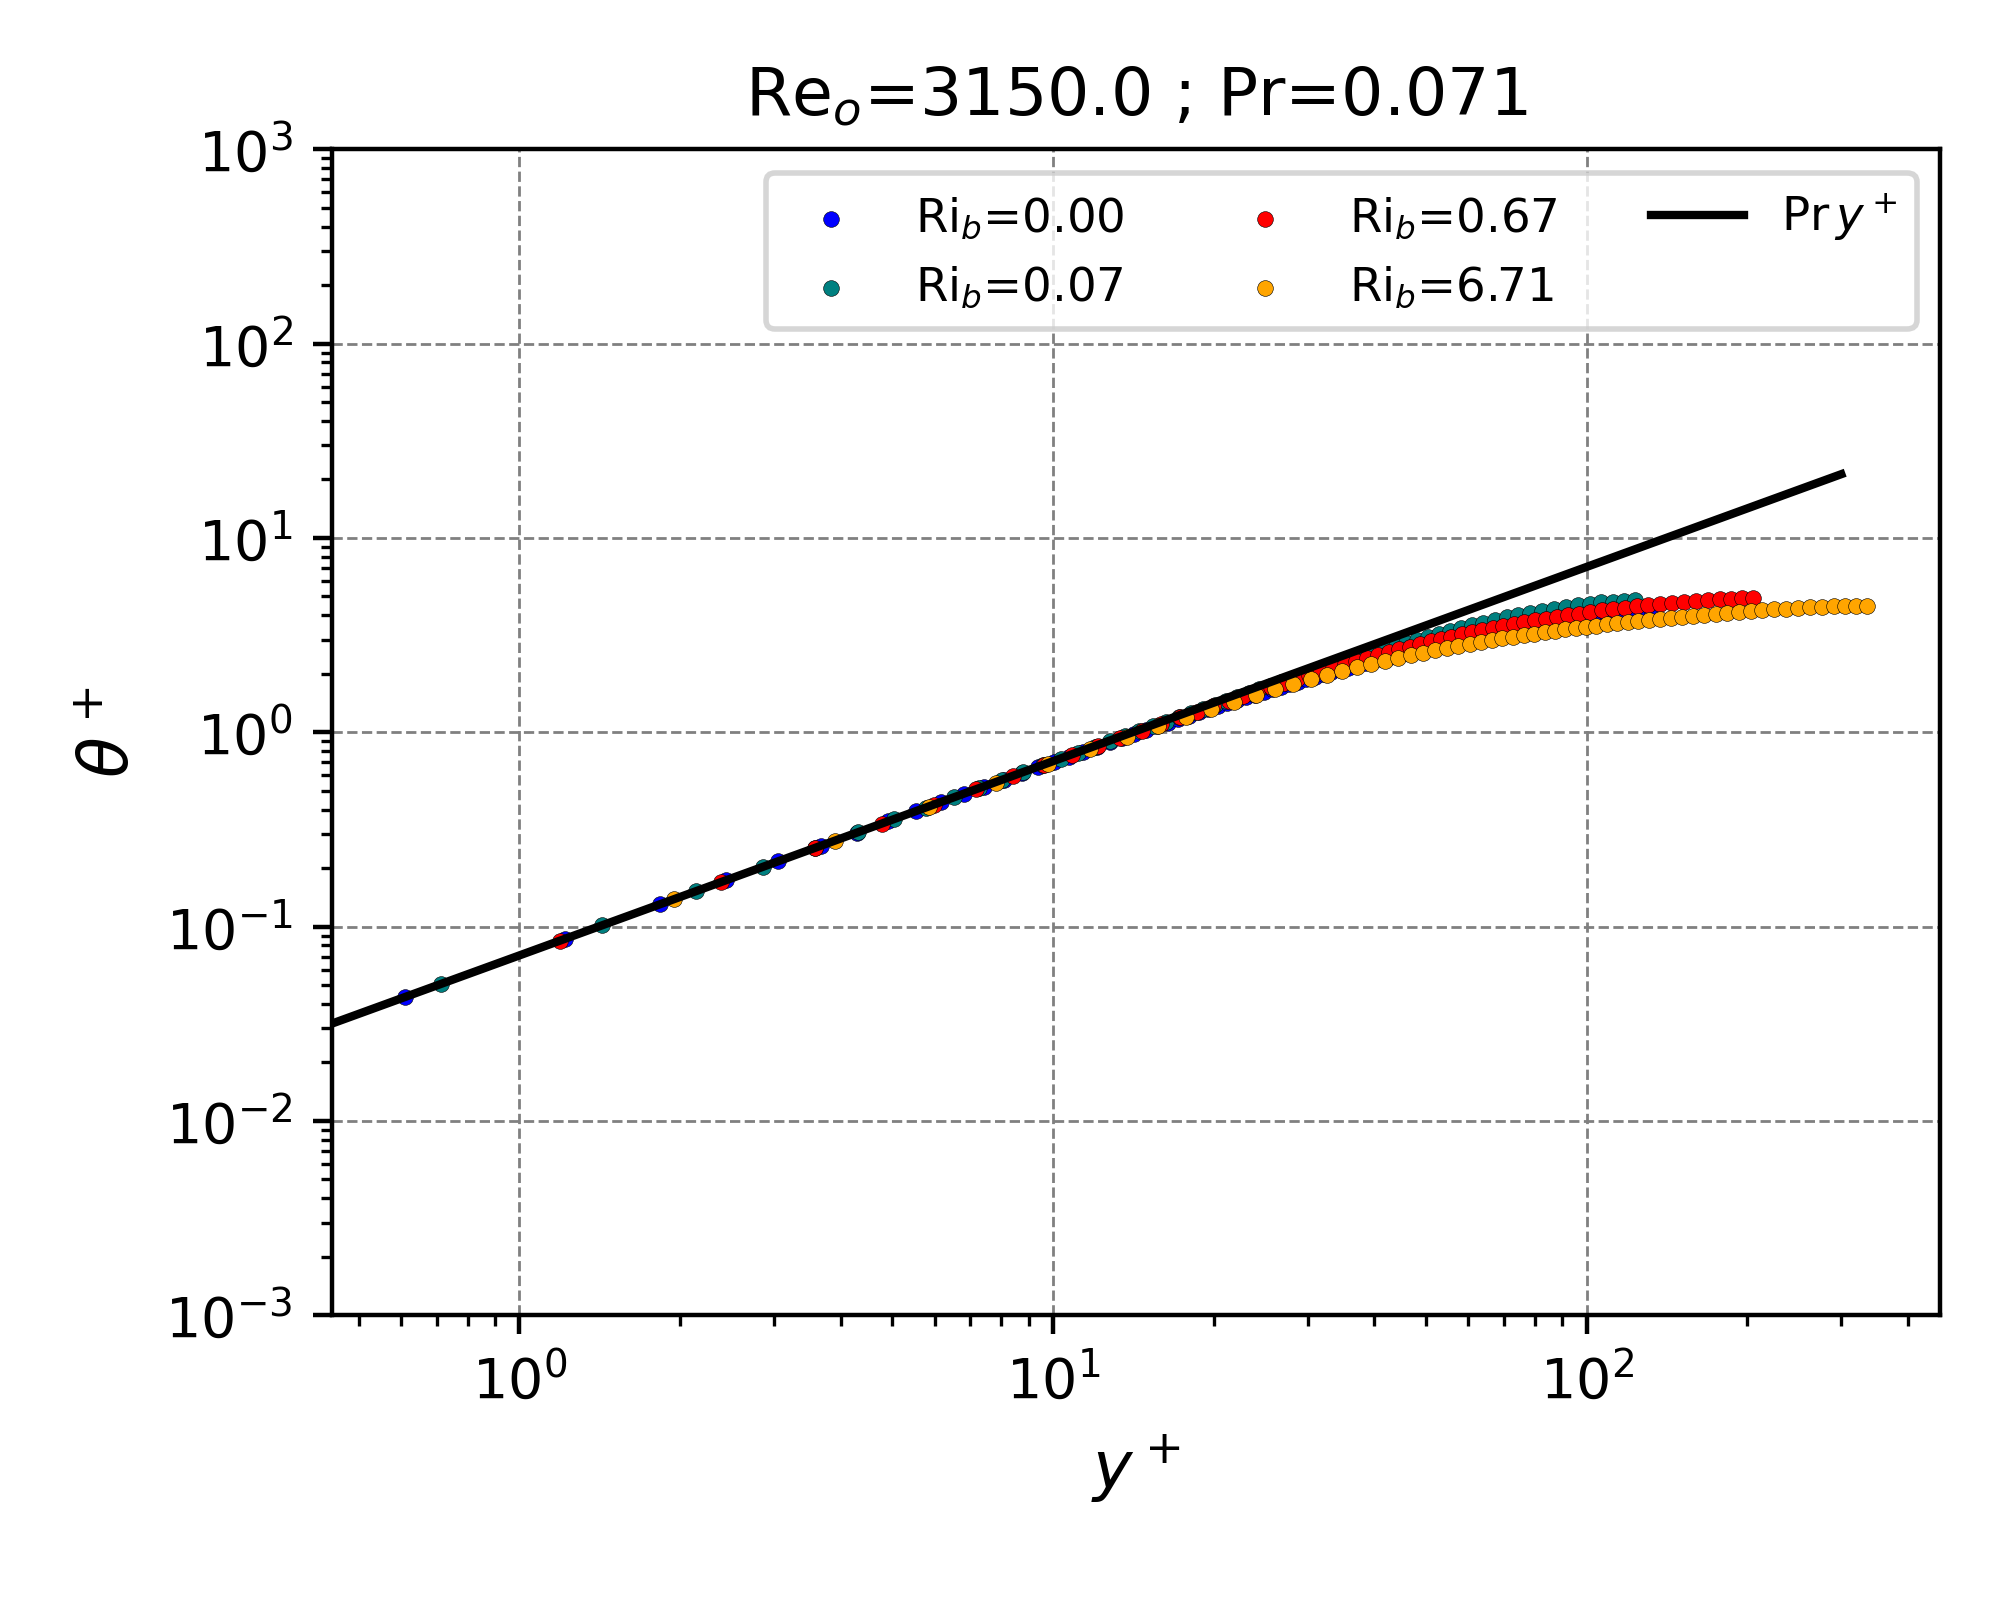
\includegraphics[width=0.45\textwidth]{figures/cap5/Re3150-Pr0071/phi_mean_plus_log_profile.png}}
  \subfloat[]{
    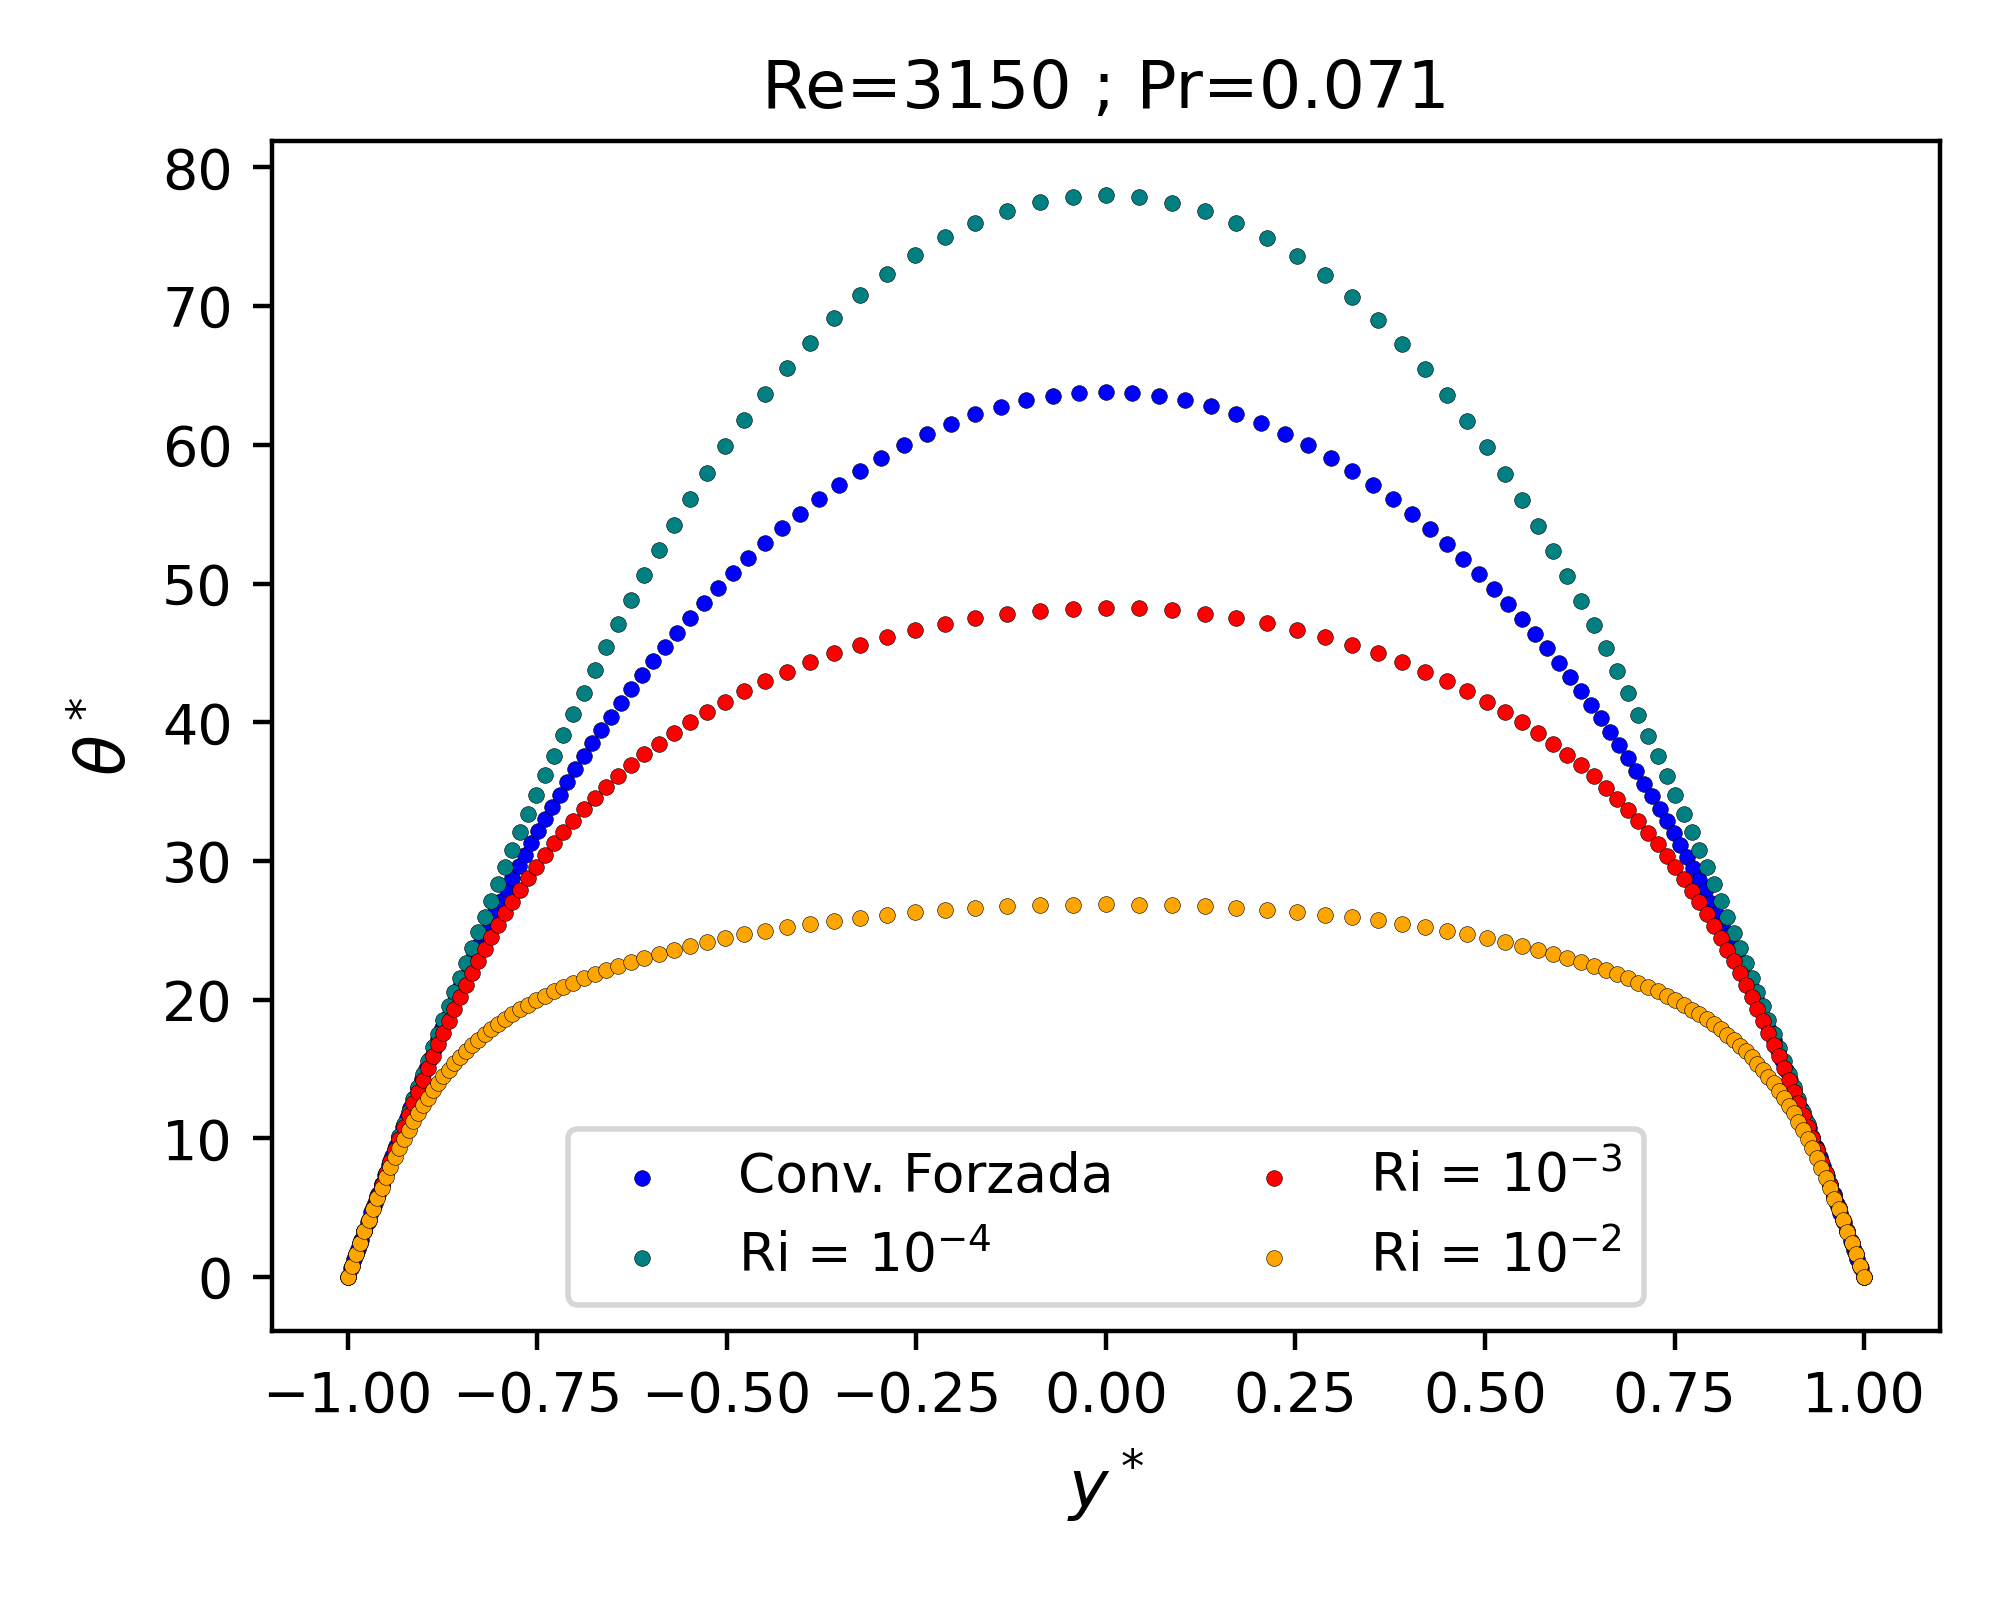
\includegraphics[width=0.45\textwidth]{figures/cap5/Re3150-Pr0071/phi_mean_profile.png}}
  \caption{}
  \label{fig:phi-Re3150-Pr0071}
\end{figure}

\begin{figure}[H]
  \centering
  \subfloat[]{
    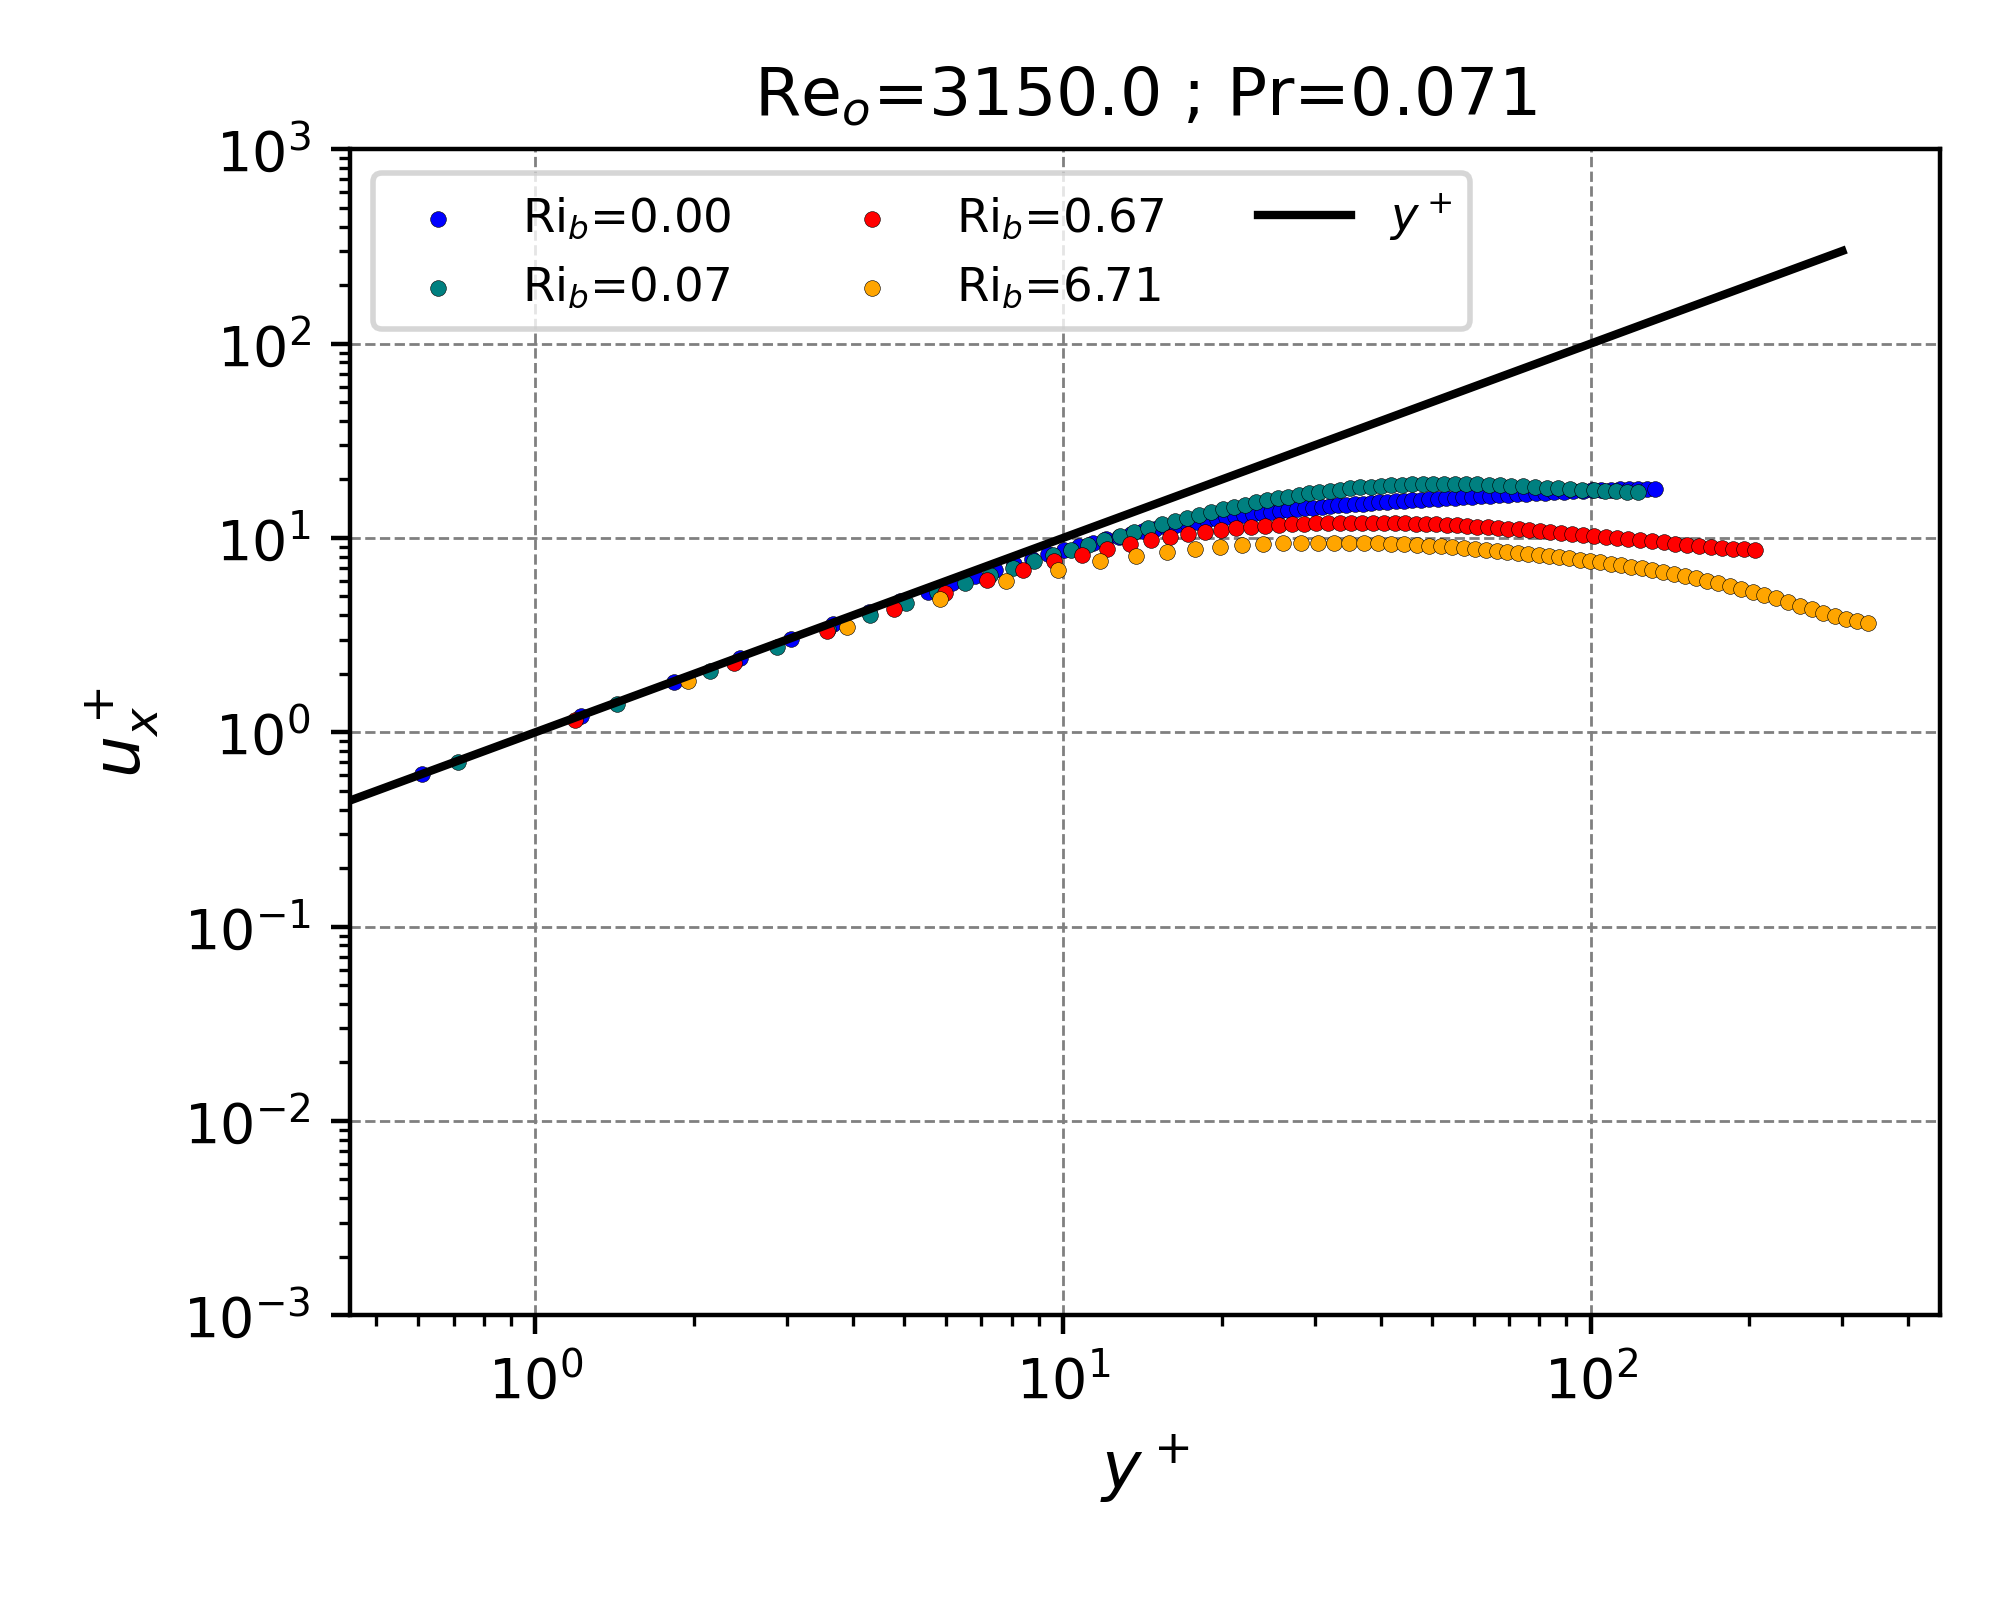
\includegraphics[width=0.45\textwidth]{figures/cap5/Re3150-Pr0071/ux_mean_plus_log_profile.png}}
  \subfloat[]{
    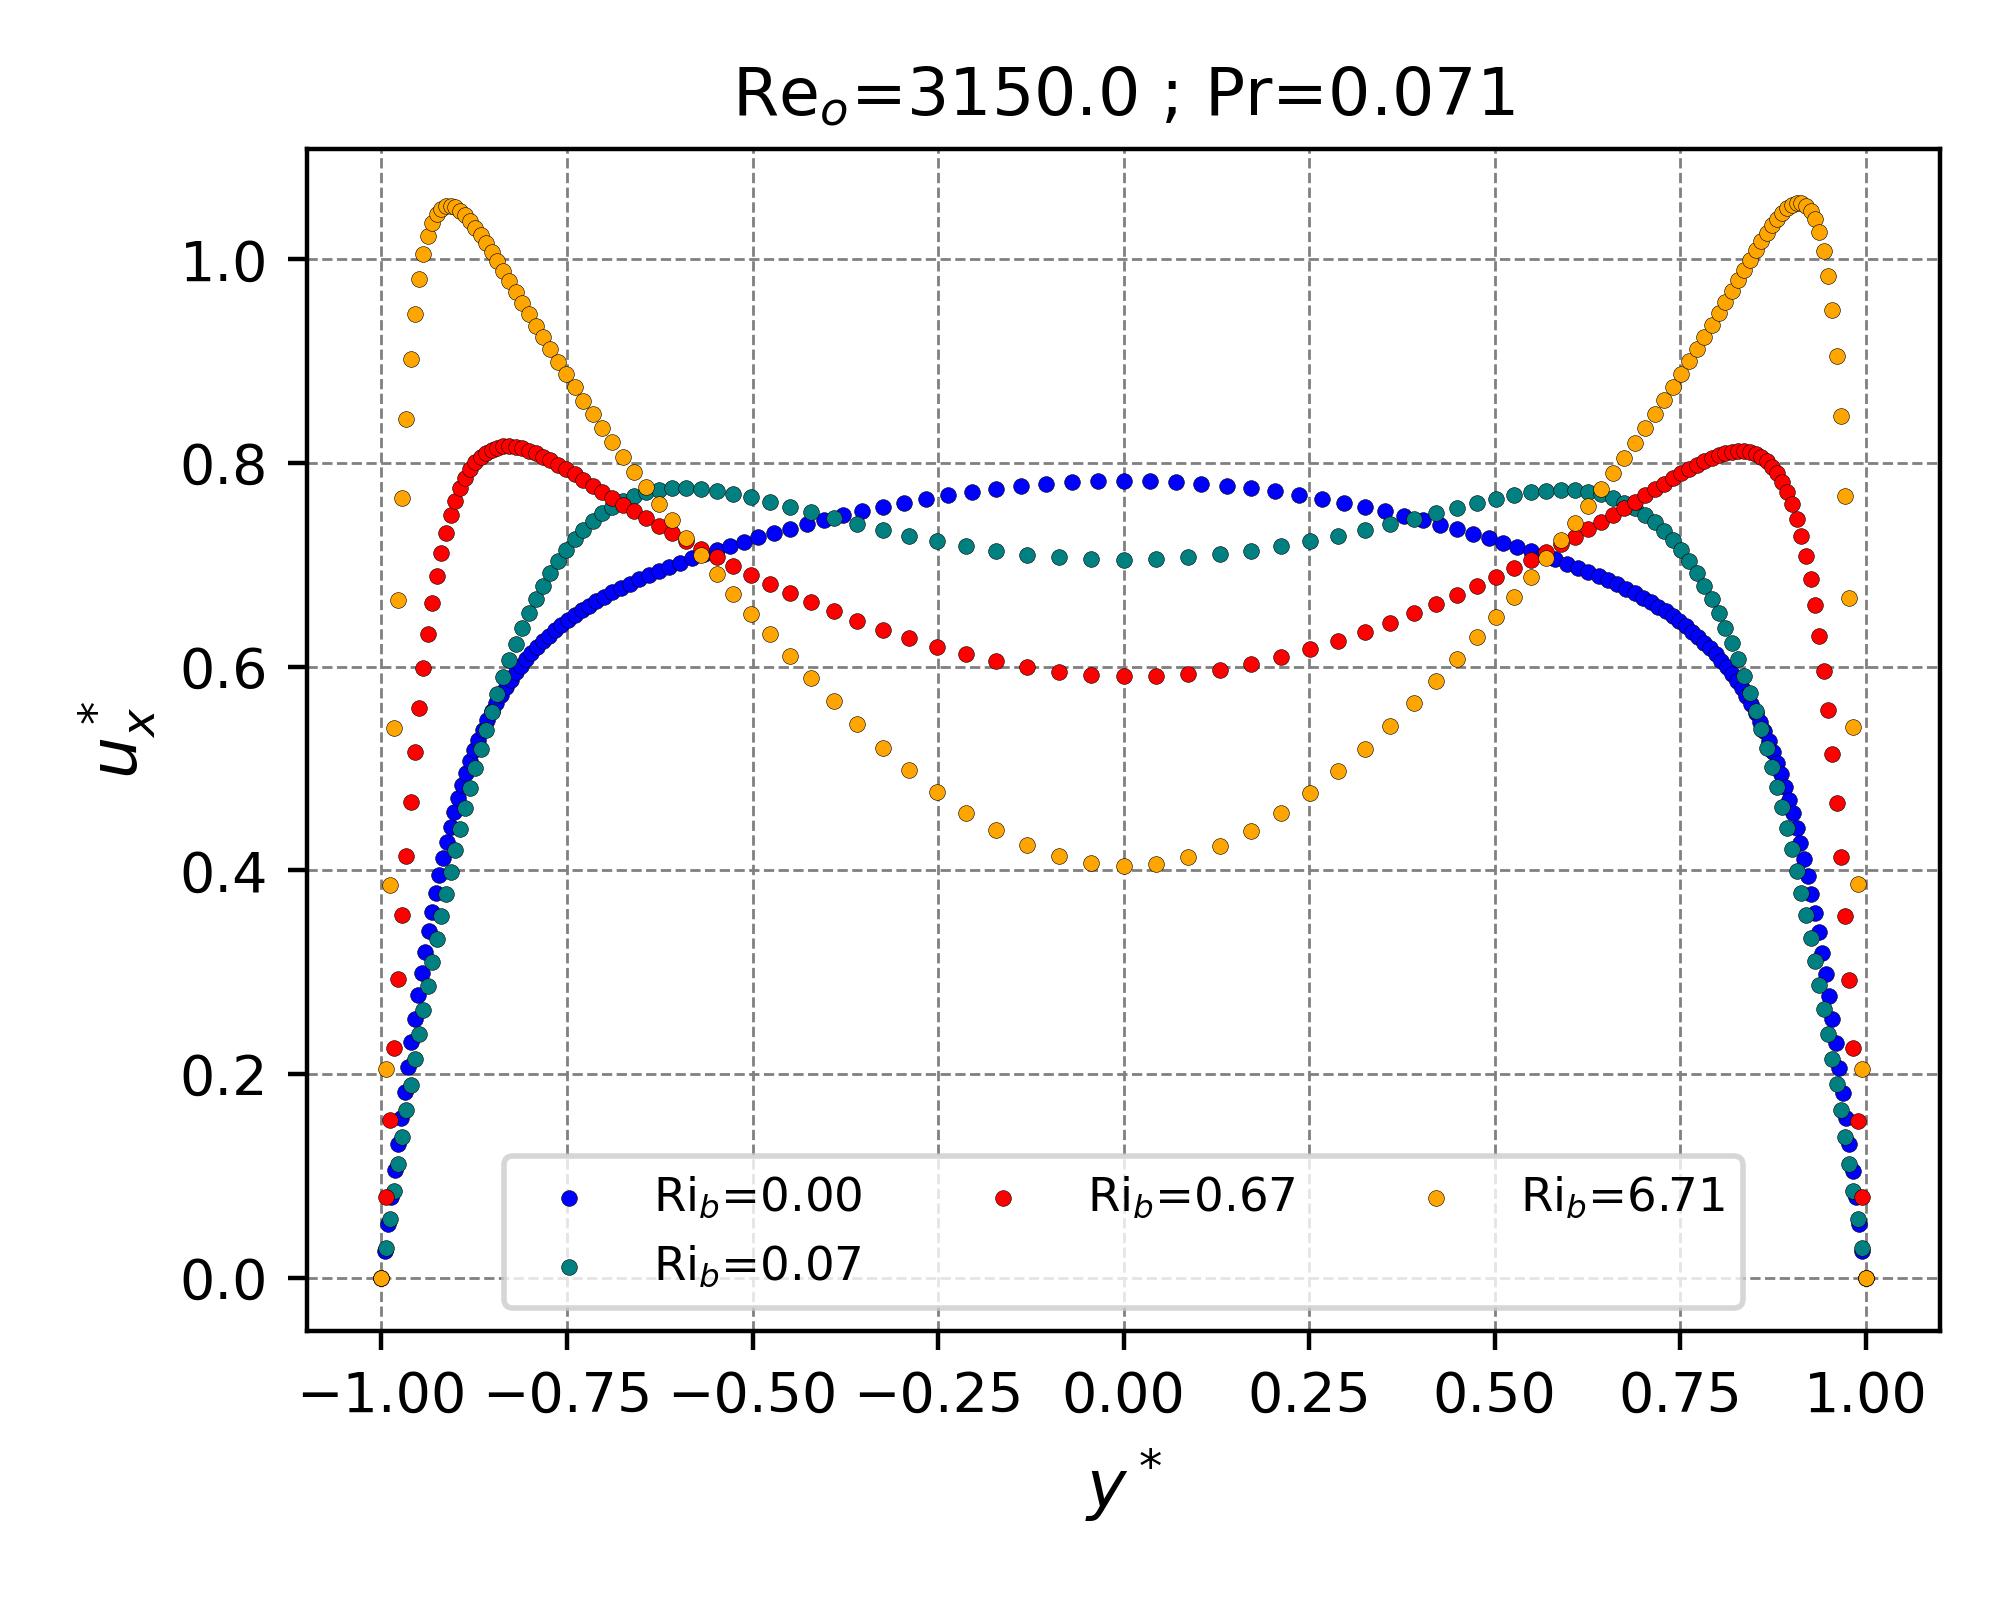
\includegraphics[width=0.45\textwidth]{figures/cap5/Re3150-Pr0071/ux_mean_profile.png}}
  \caption{}
  \label{fig:ux-Re3150-Pr0071}
\end{figure}

%% ==============================================================
%%  Re = 4278, Pr = 0.71
%% ==============================================================

\section{$\text{Re}=4278$ y $\text{Pr}=0.71$}

\begin{figure}[H]
  \centering
  \subfloat[]{
    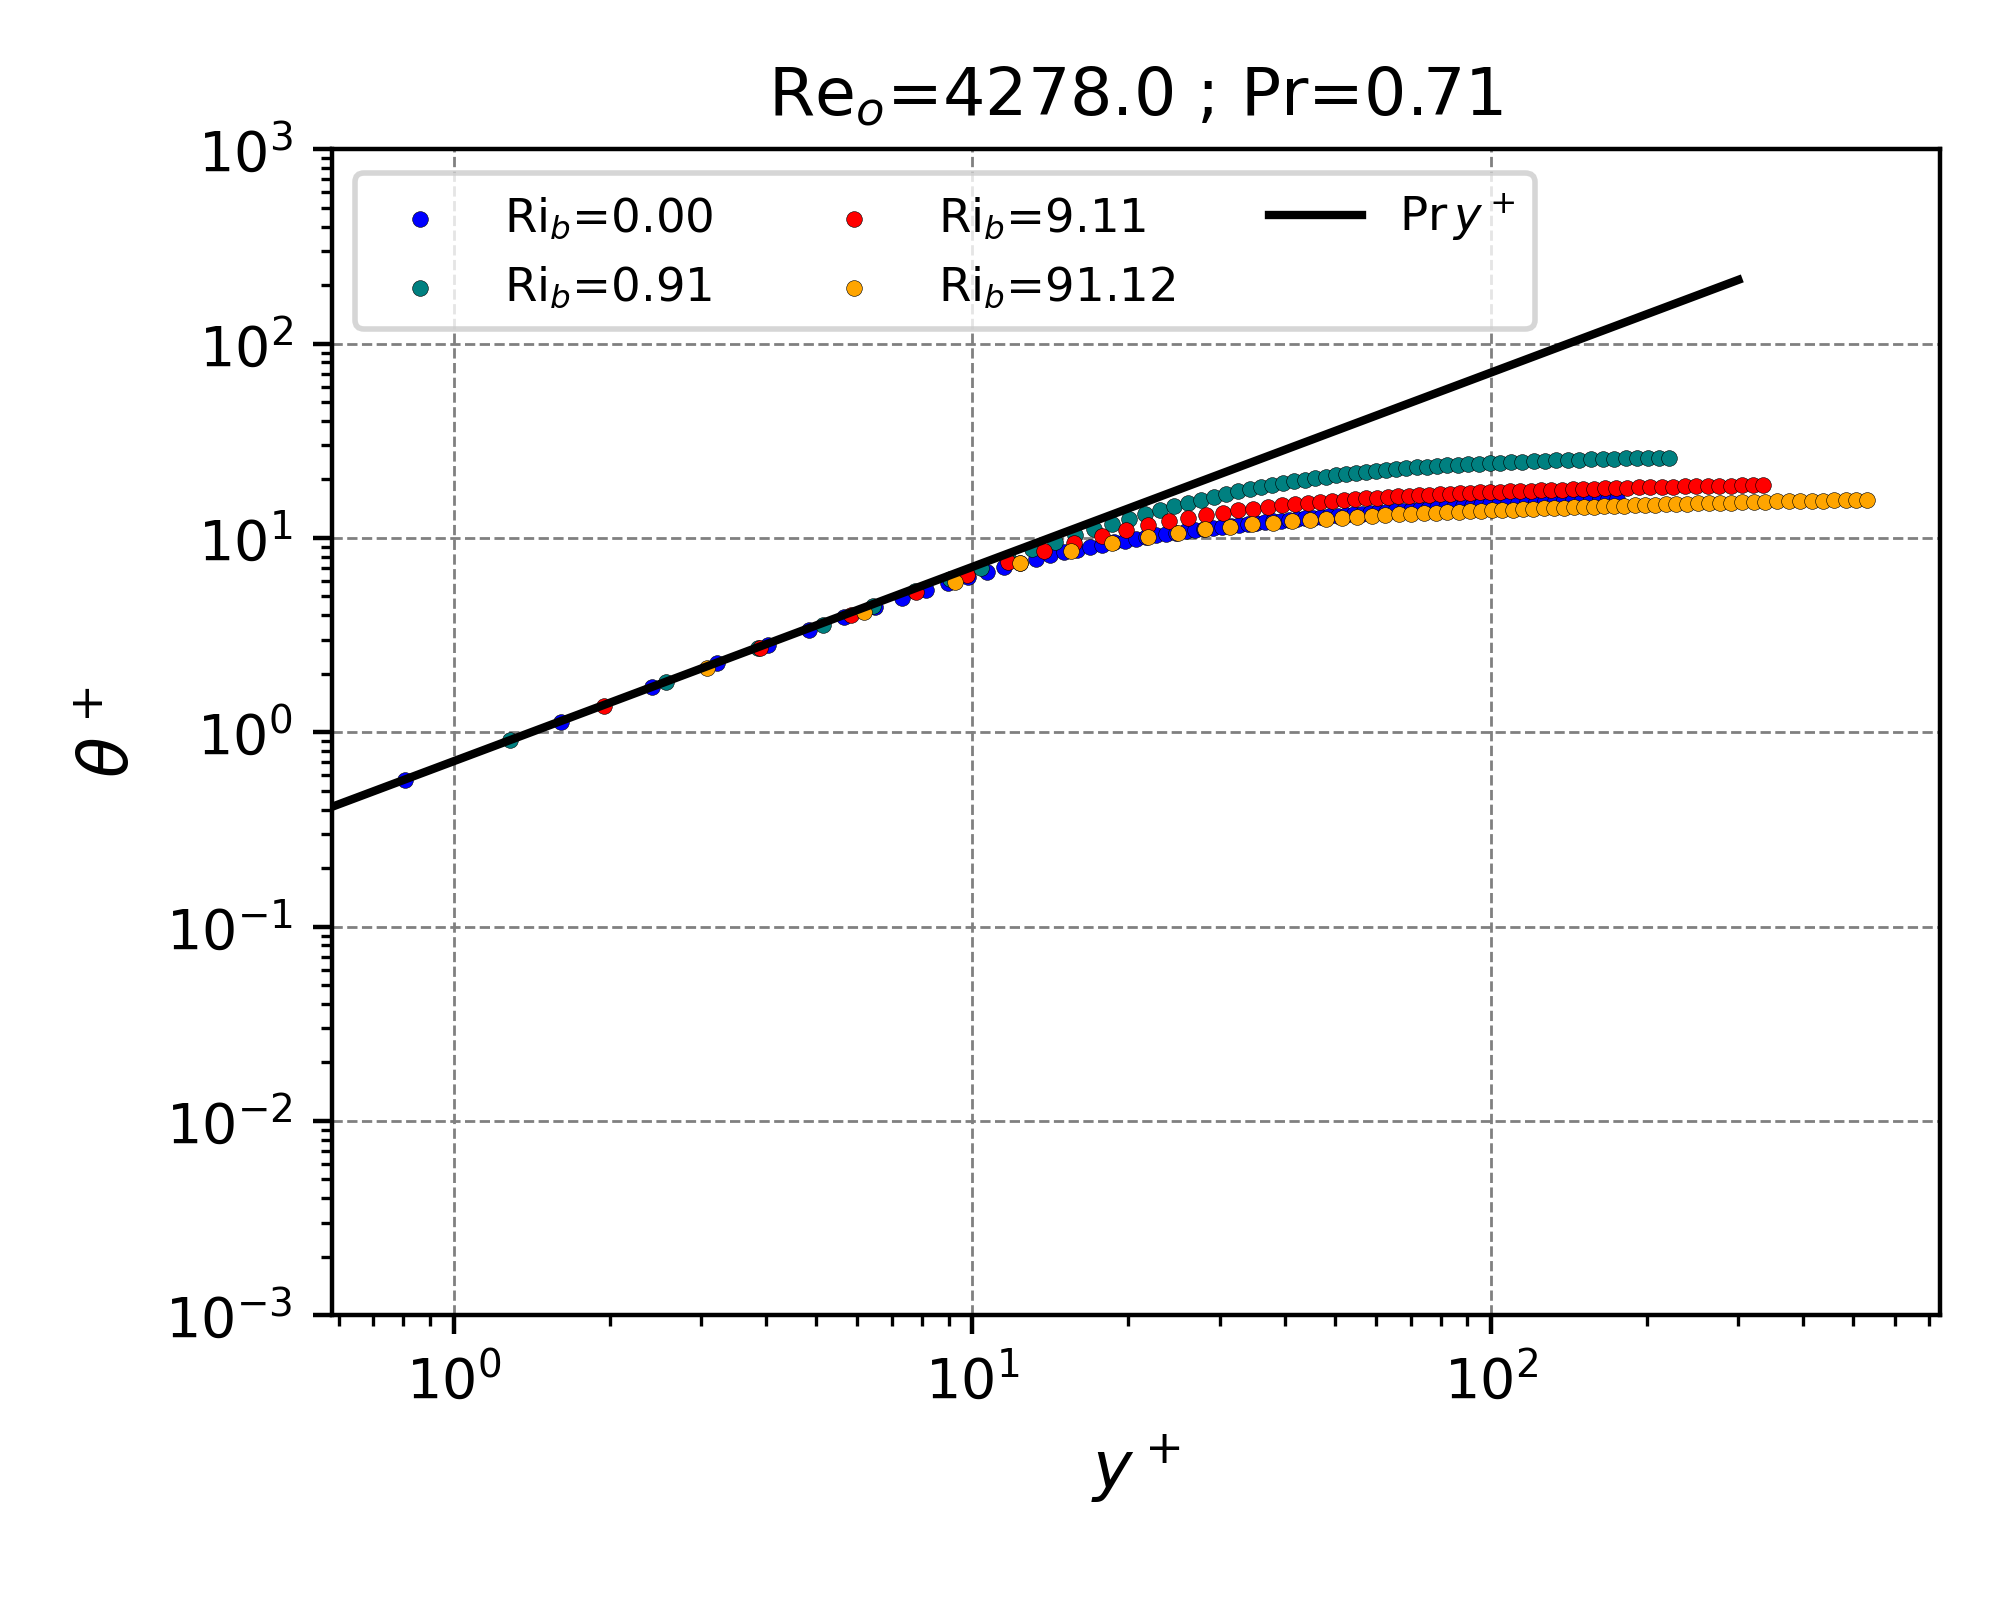
\includegraphics[width=0.45\textwidth]{figures/cap5/Re4278-Pr071/phi_mean_plus_log_profile.png}}
  \subfloat[]{
    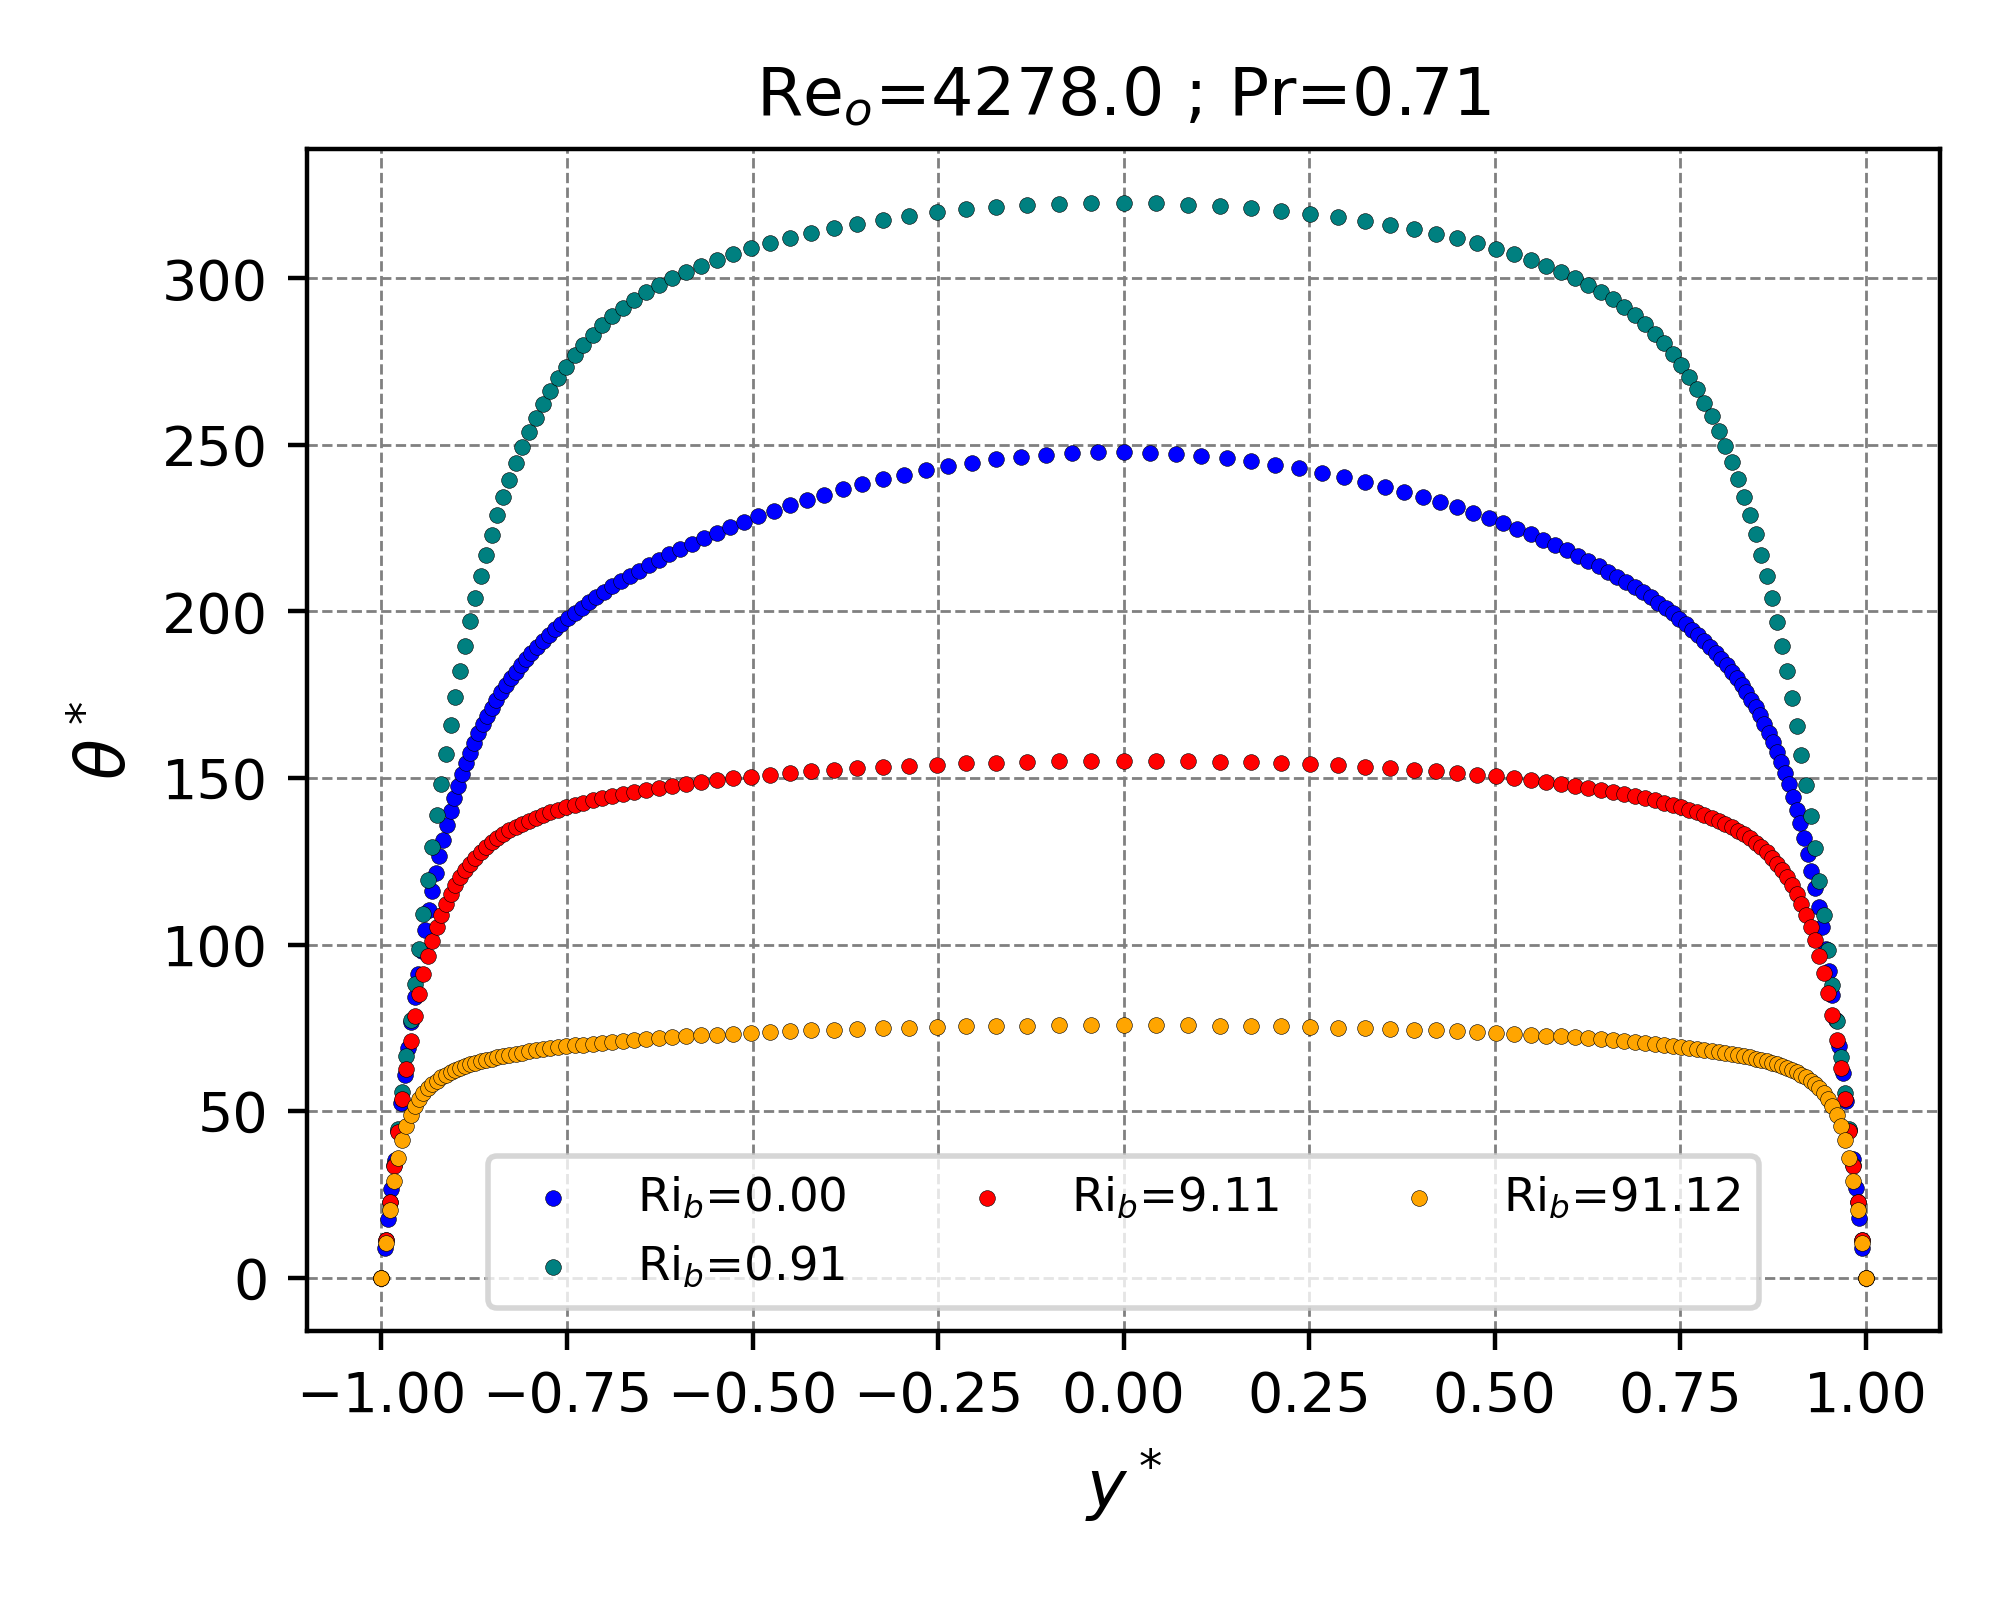
\includegraphics[width=0.45\textwidth]{figures/cap5/Re4278-Pr071/phi_mean_profile.png}}
  \caption{}
  \label{fig:phi-Re4278-Pr071}
\end{figure}

\begin{figure}[H]
  \centering
  \subfloat[]{
    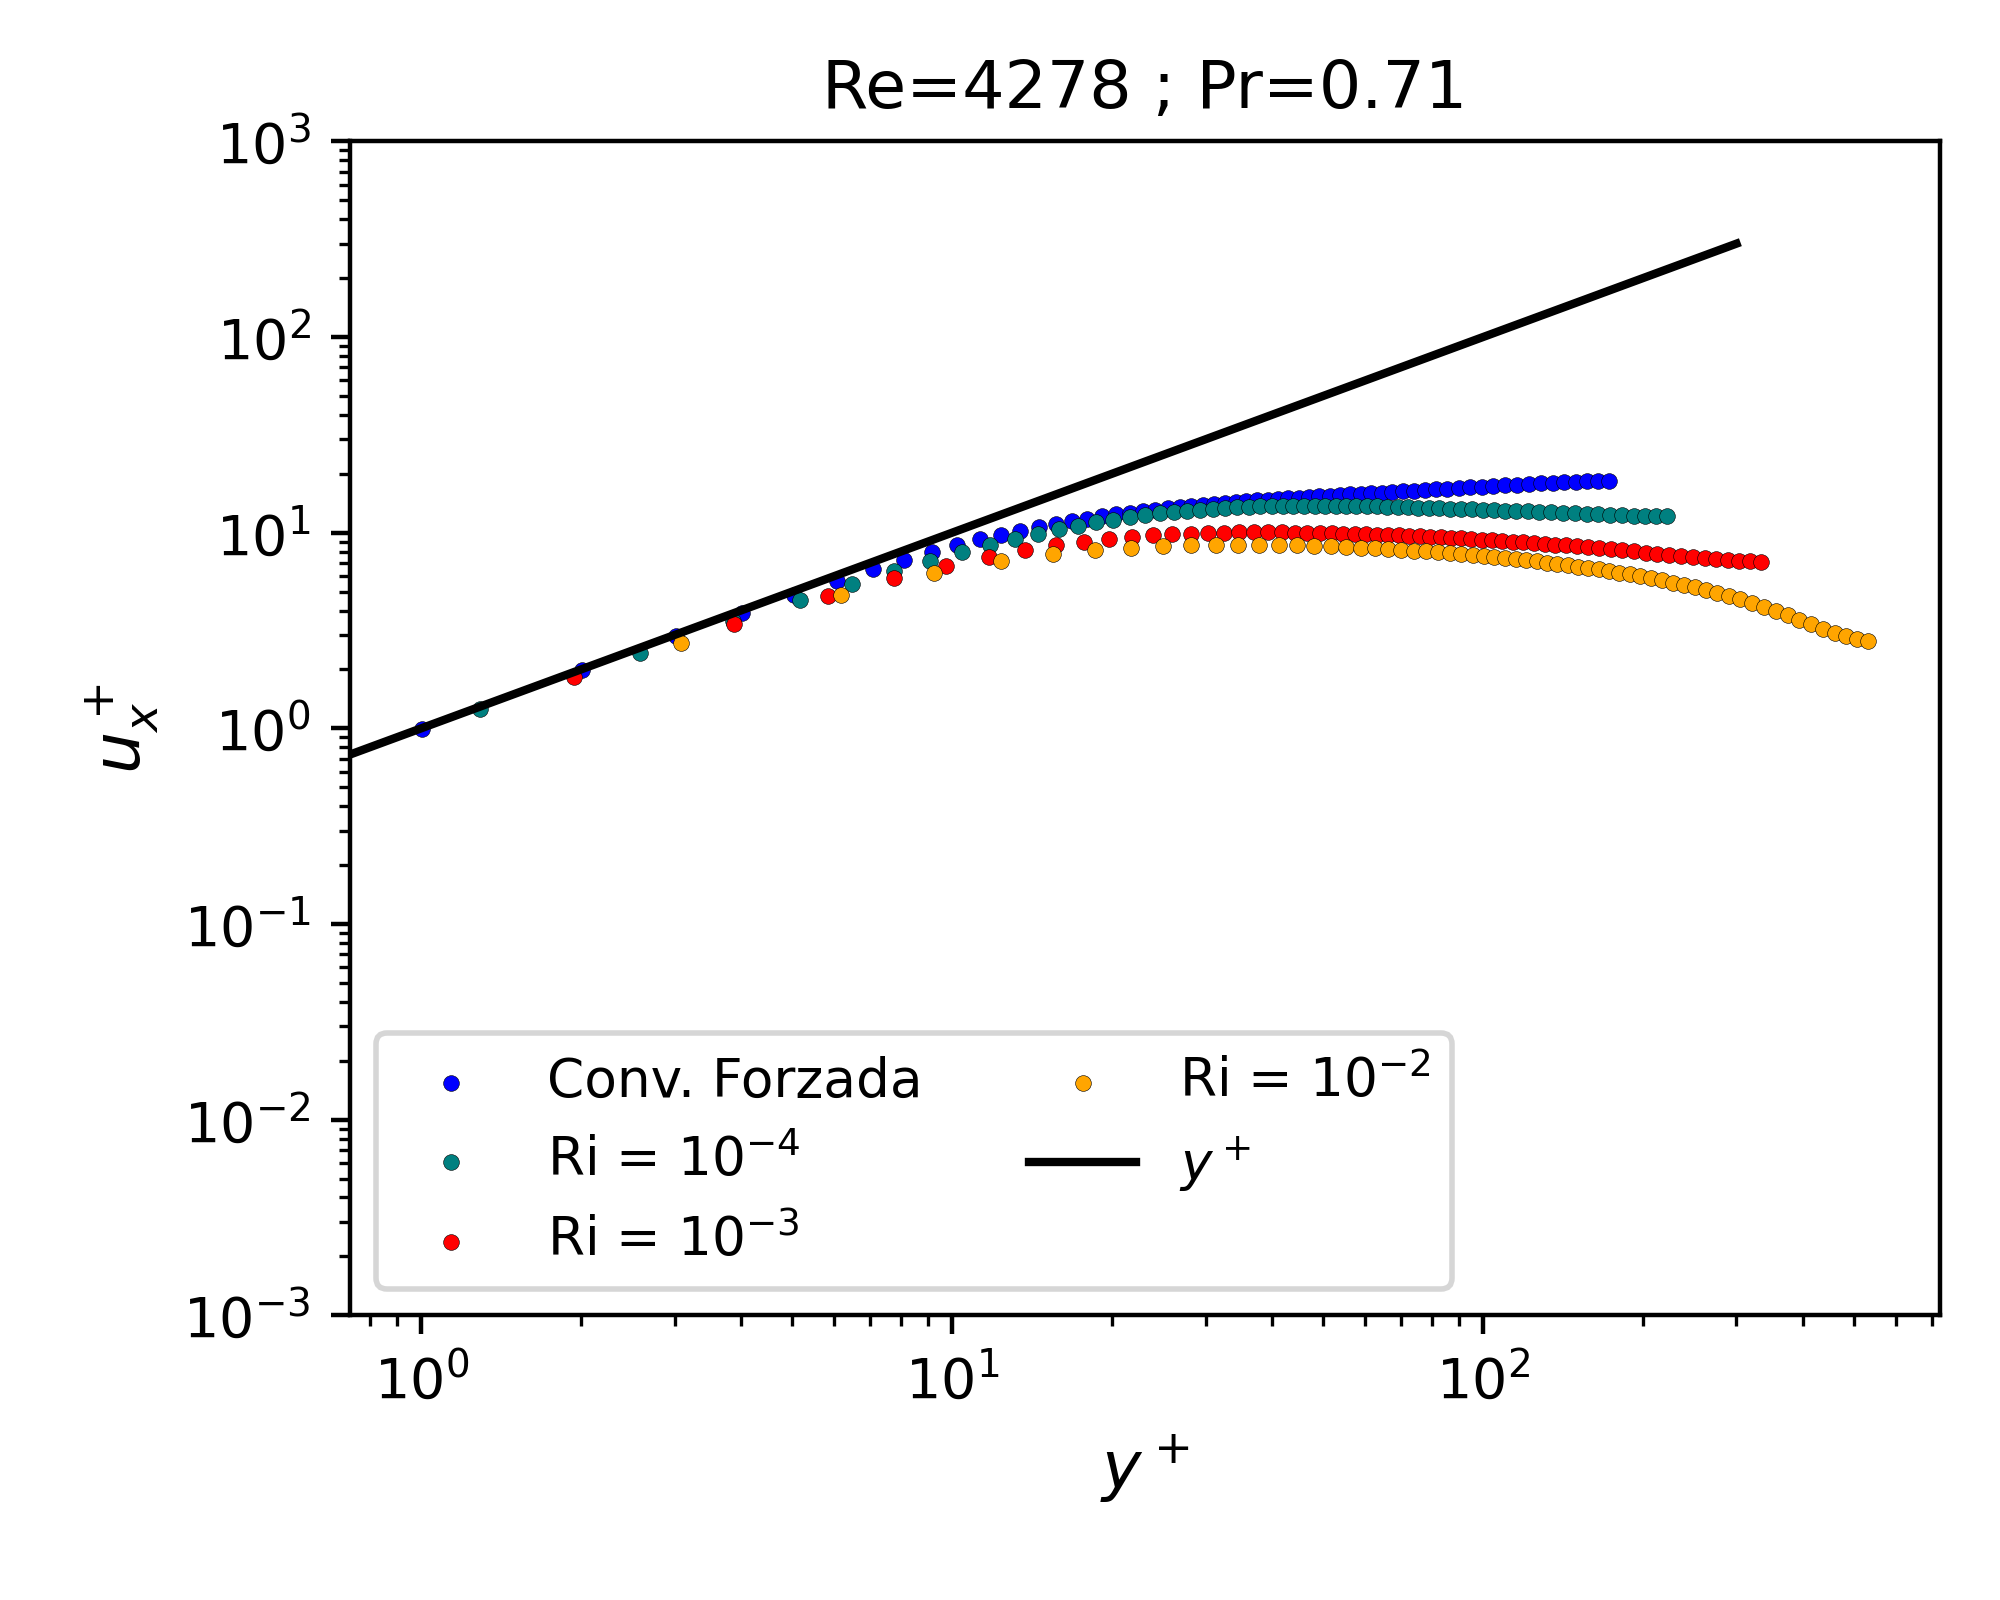
\includegraphics[width=0.45\textwidth]{figures/cap5/Re4278-Pr071/ux_mean_plus_log_profile.png}}
  \subfloat[]{
    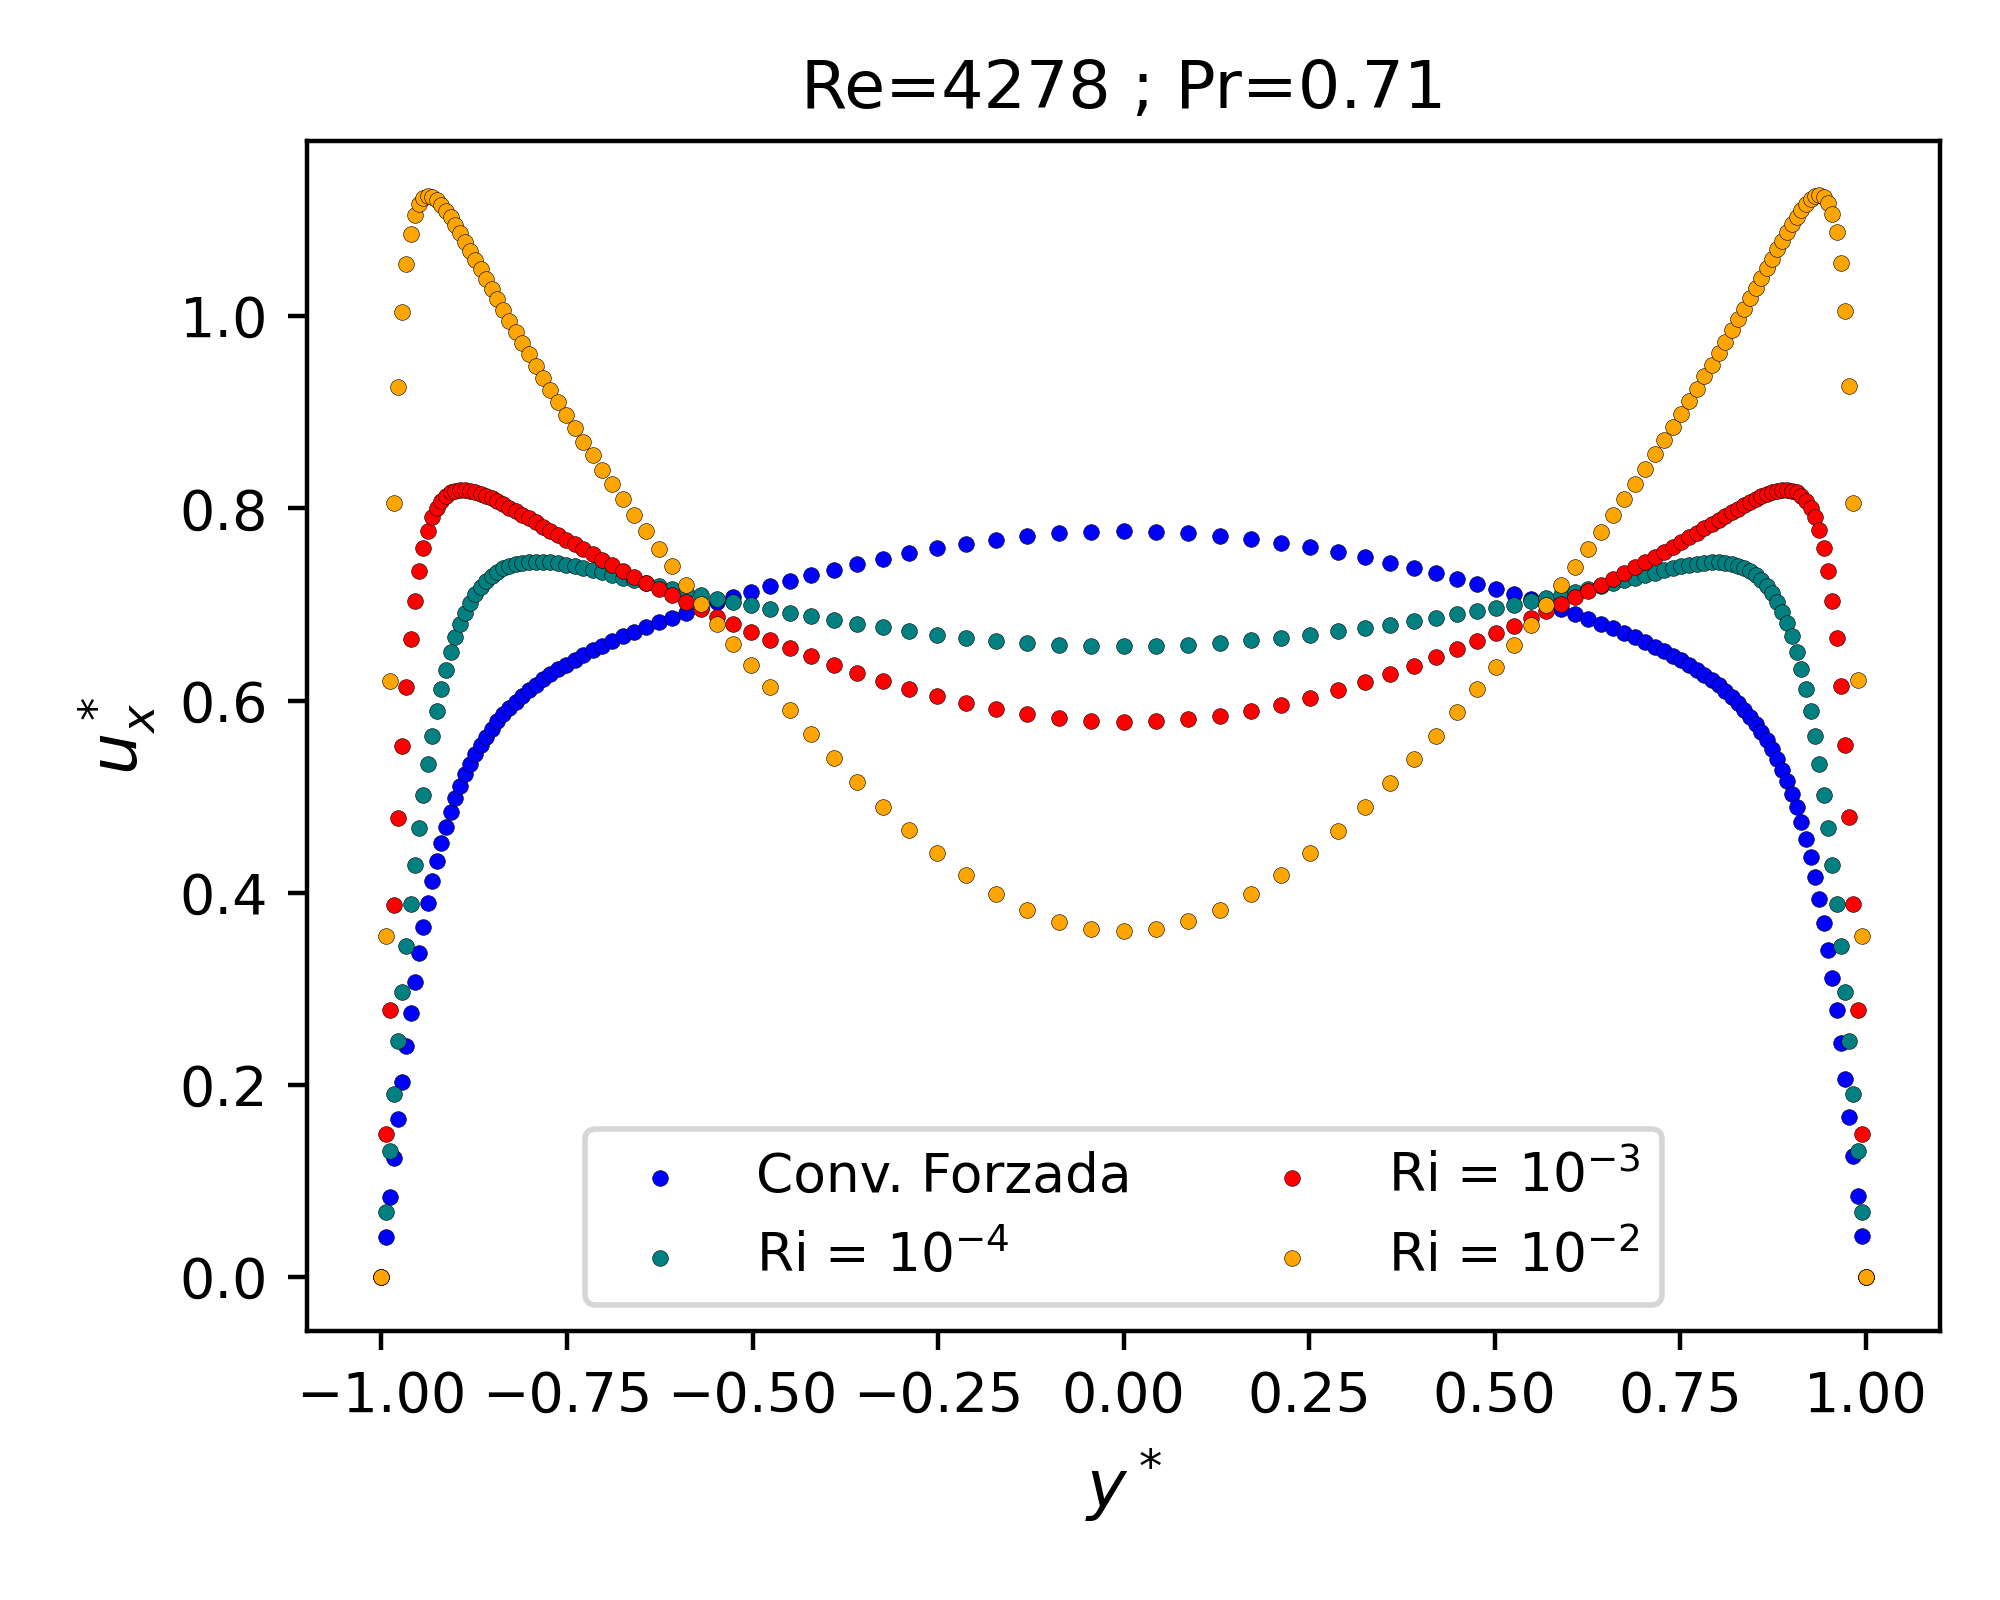
\includegraphics[width=0.45\textwidth]{figures/cap5/Re4278-Pr071/ux_mean_profile.png}}
  \caption{}
  \label{fig:ux-Re4278-Pr071}
\end{figure}

%% ==============================================================
%%  Re = 4278, Pr = 0.071
%% ==============================================================

\section{$\text{Re}=4278$ y $\text{Pr}=0.071$}

\begin{figure}[H]
  \centering
  \subfloat[]{
    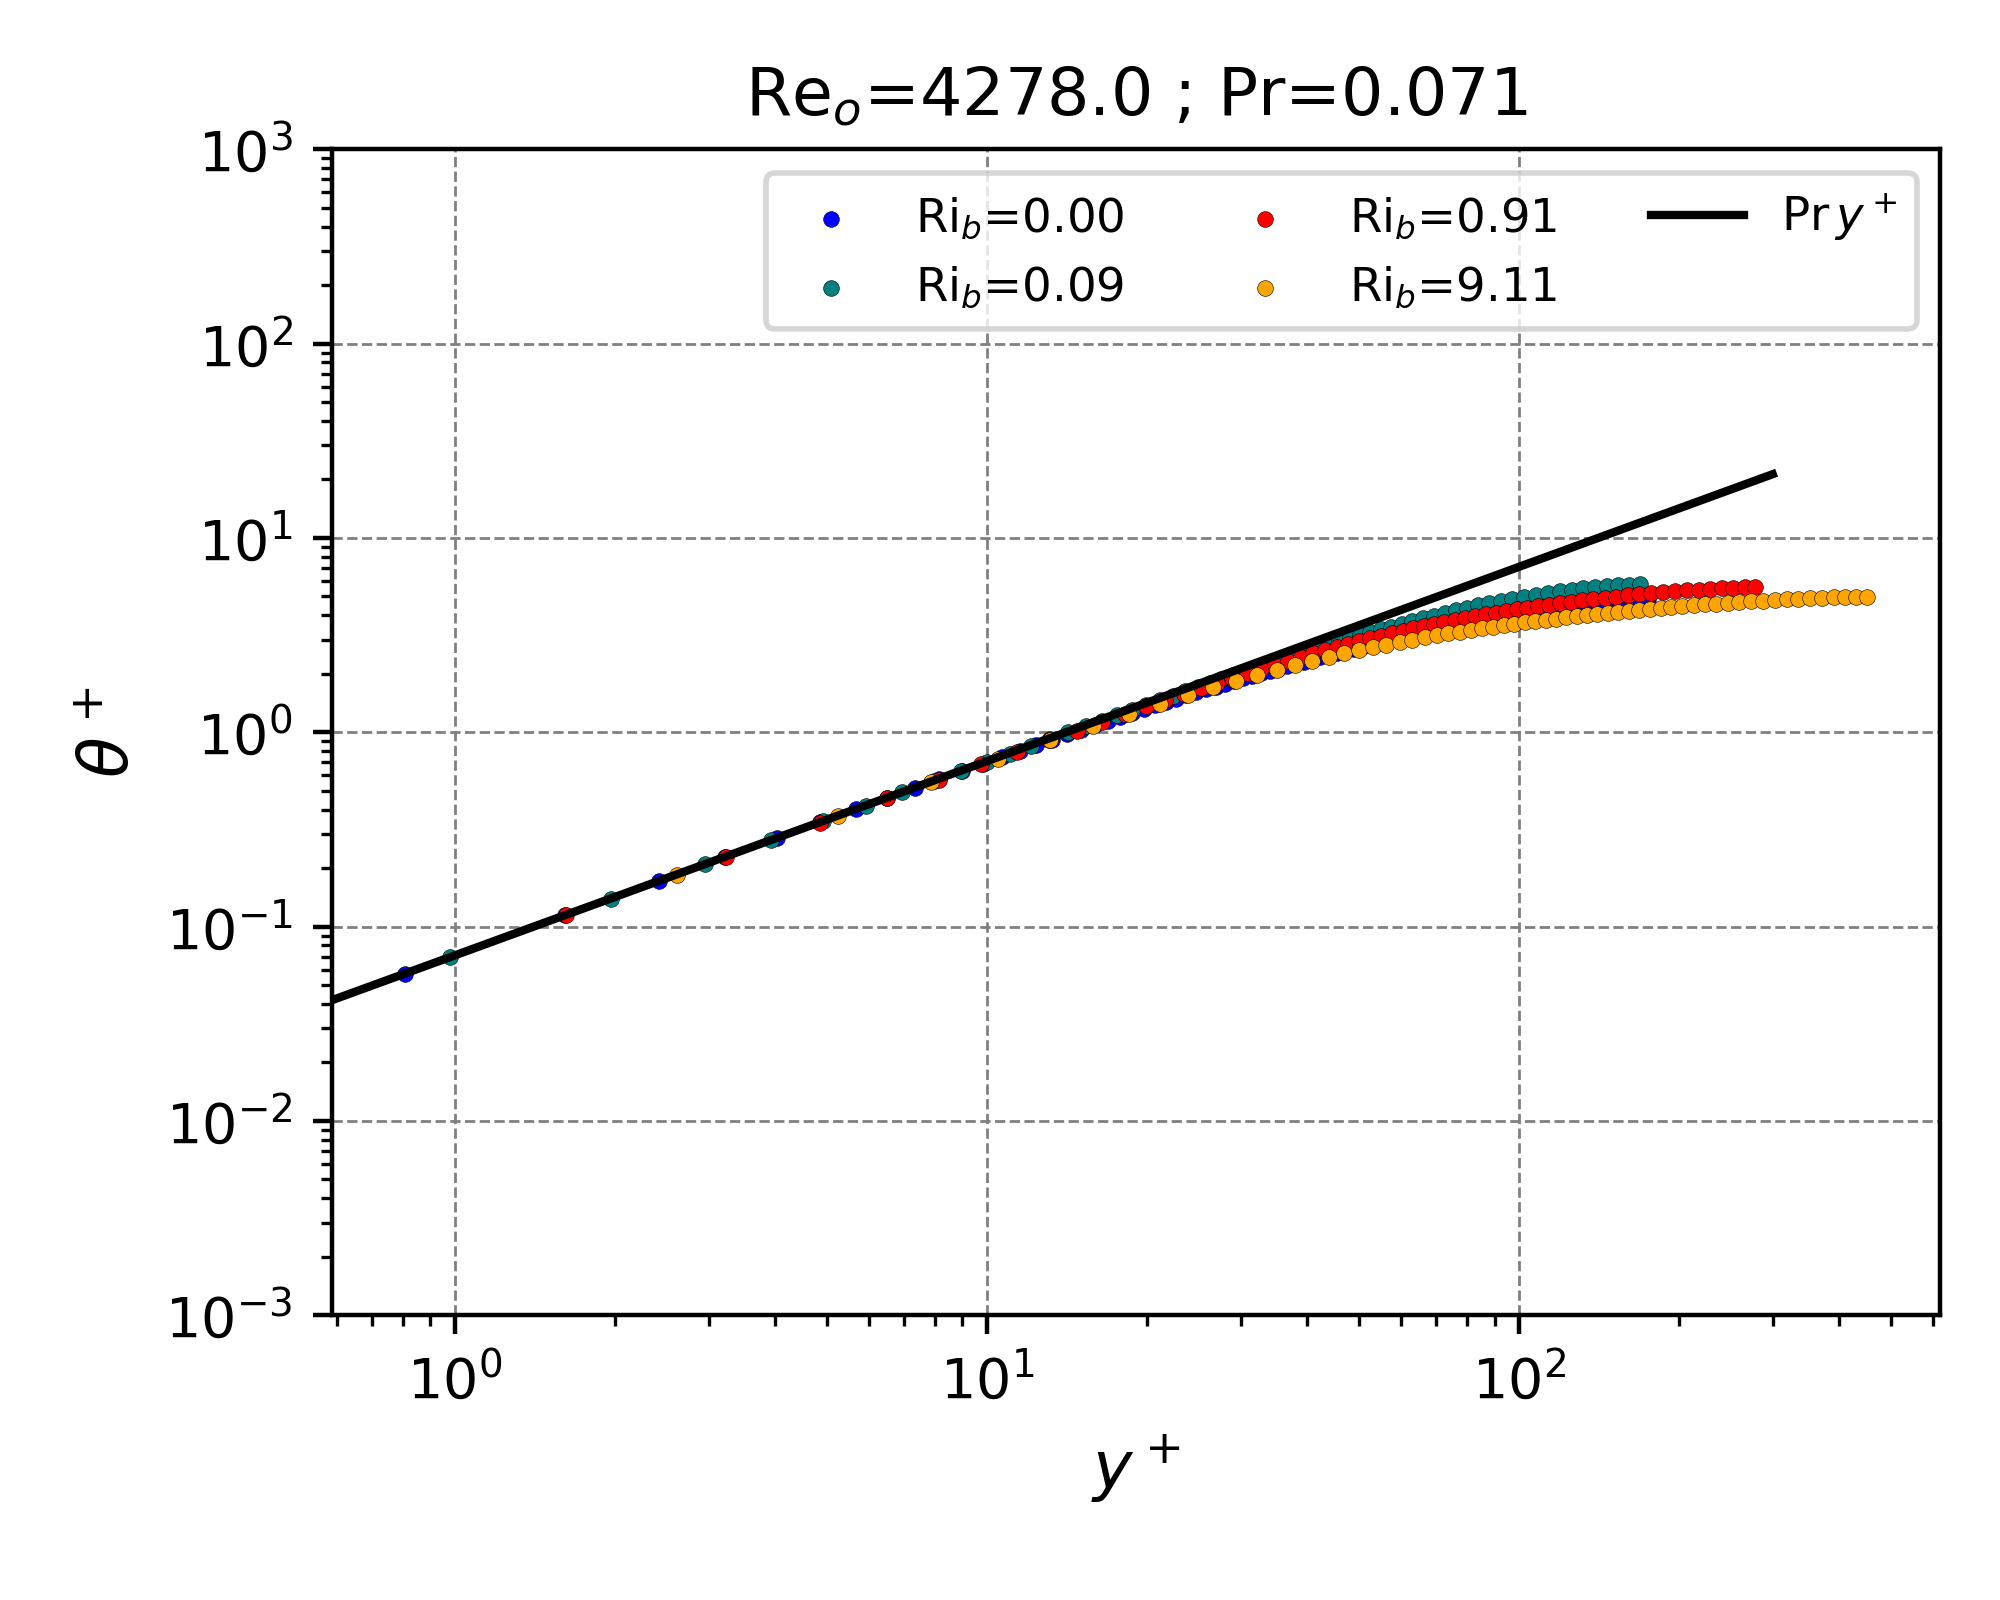
\includegraphics[width=0.45\textwidth]{figures/cap5/Re4278-Pr0071/phi_mean_plus_log_profile.png}}
  \subfloat[]{
    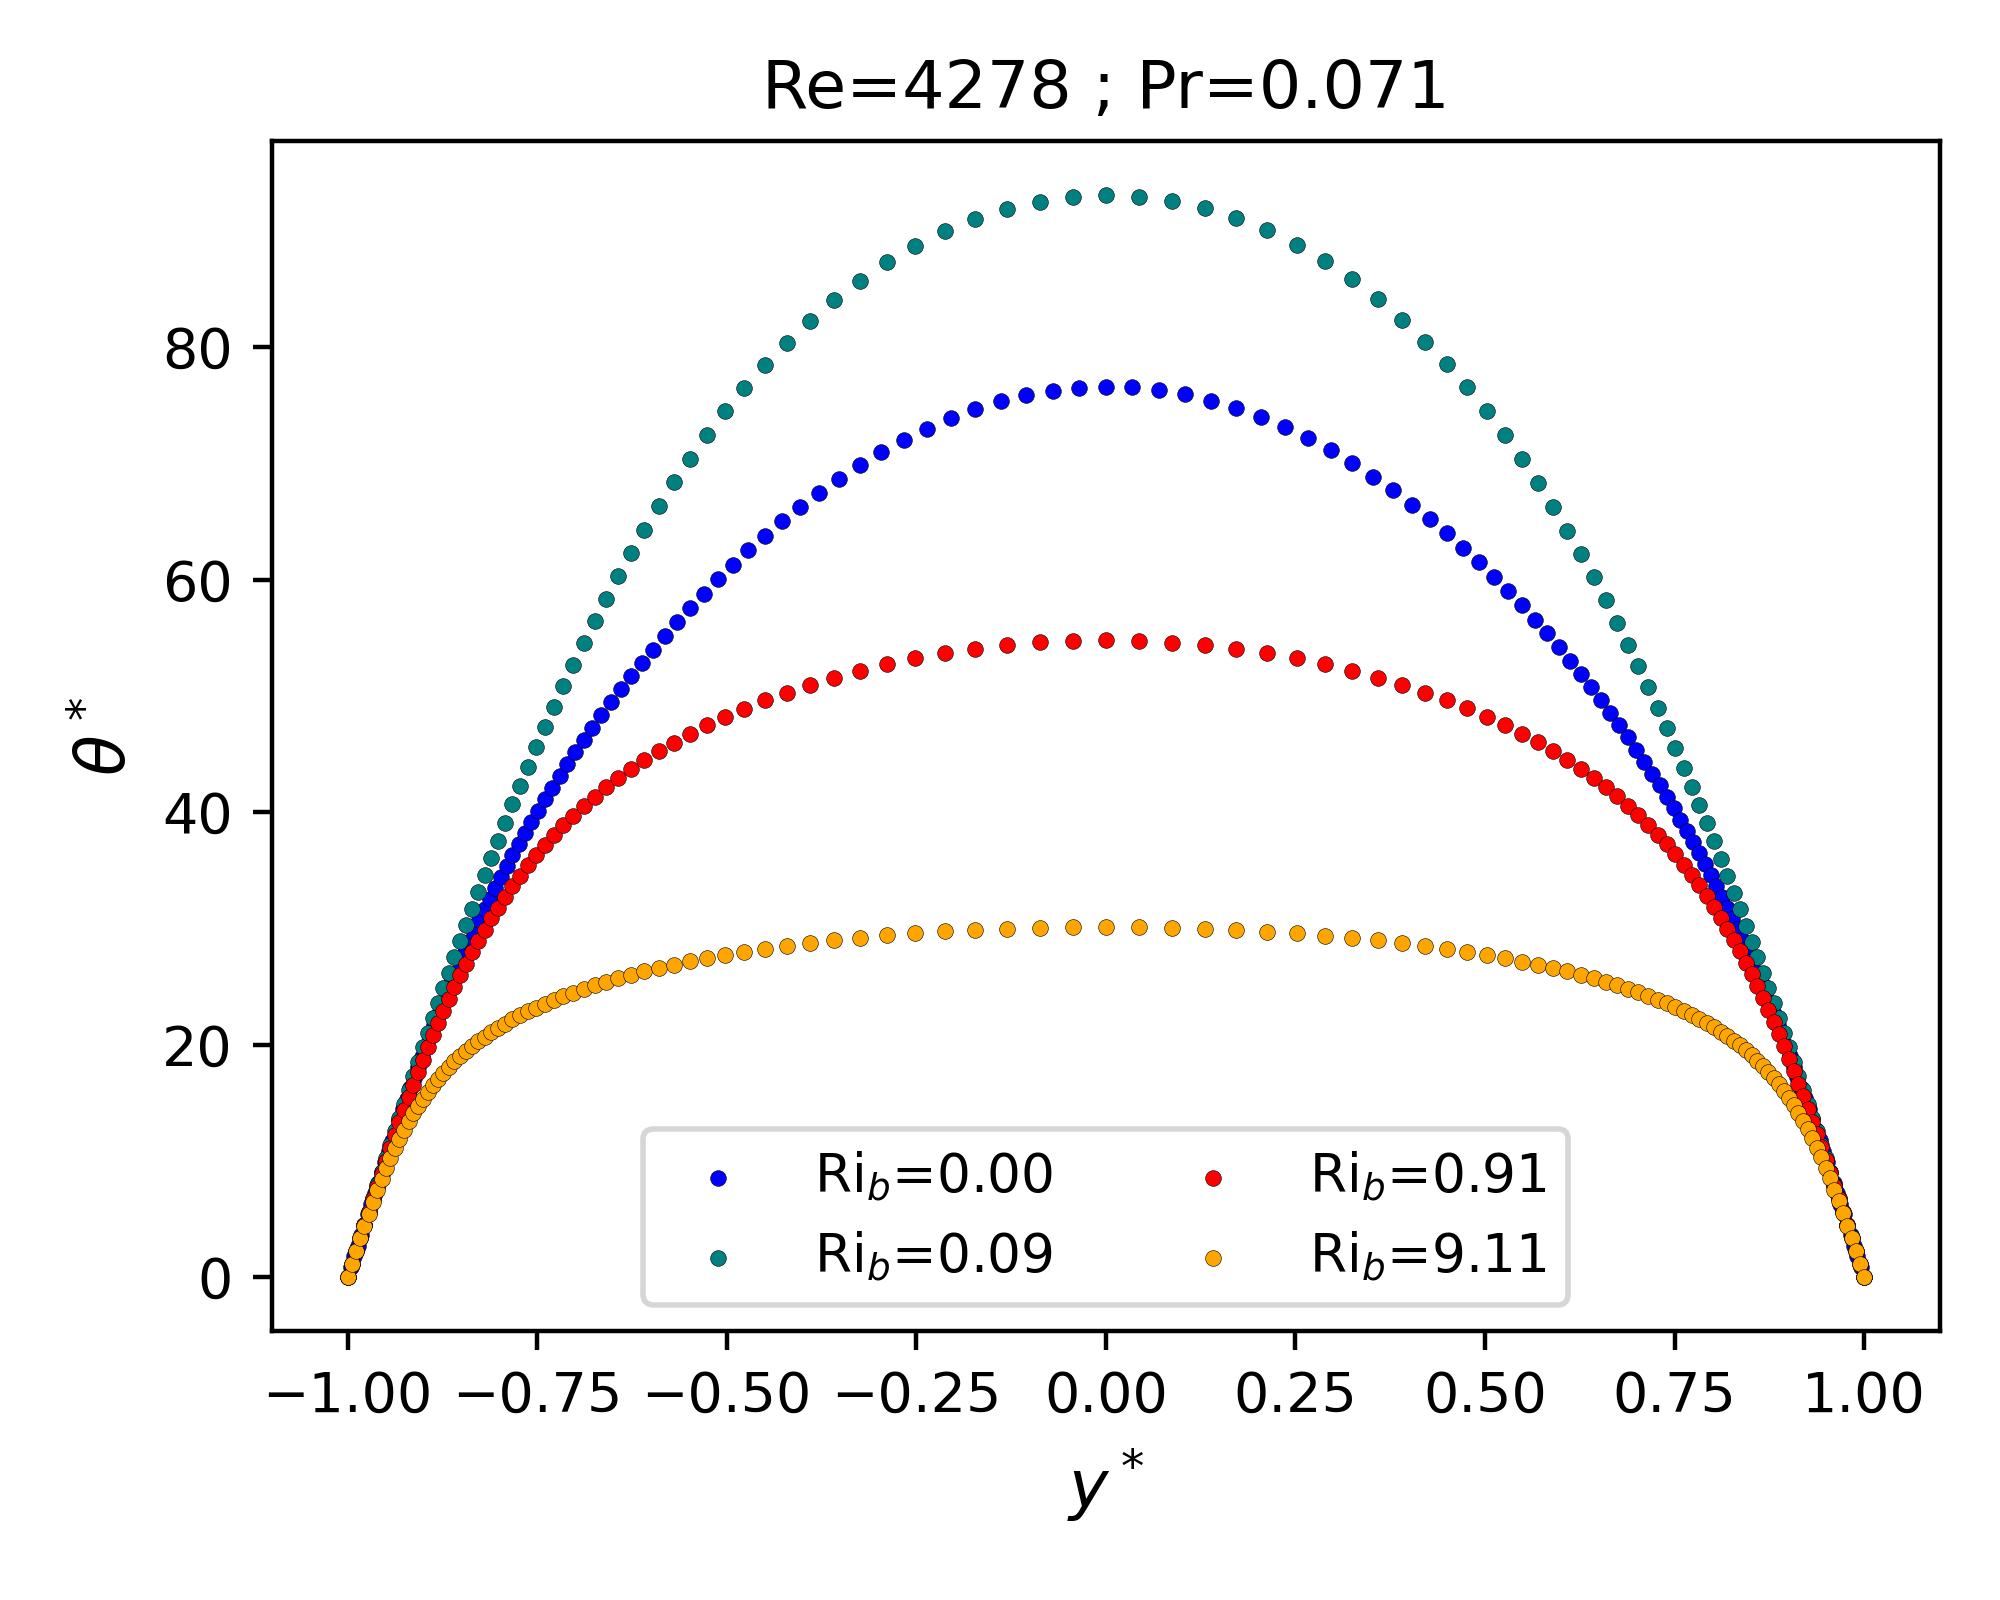
\includegraphics[width=0.45\textwidth]{figures/cap5/Re4278-Pr0071/phi_mean_profile.png}}
  \caption{}
  \label{fig:phi-Re4278-Pr0071}
\end{figure}

\begin{figure}[H]
  \centering
  \subfloat[]{
    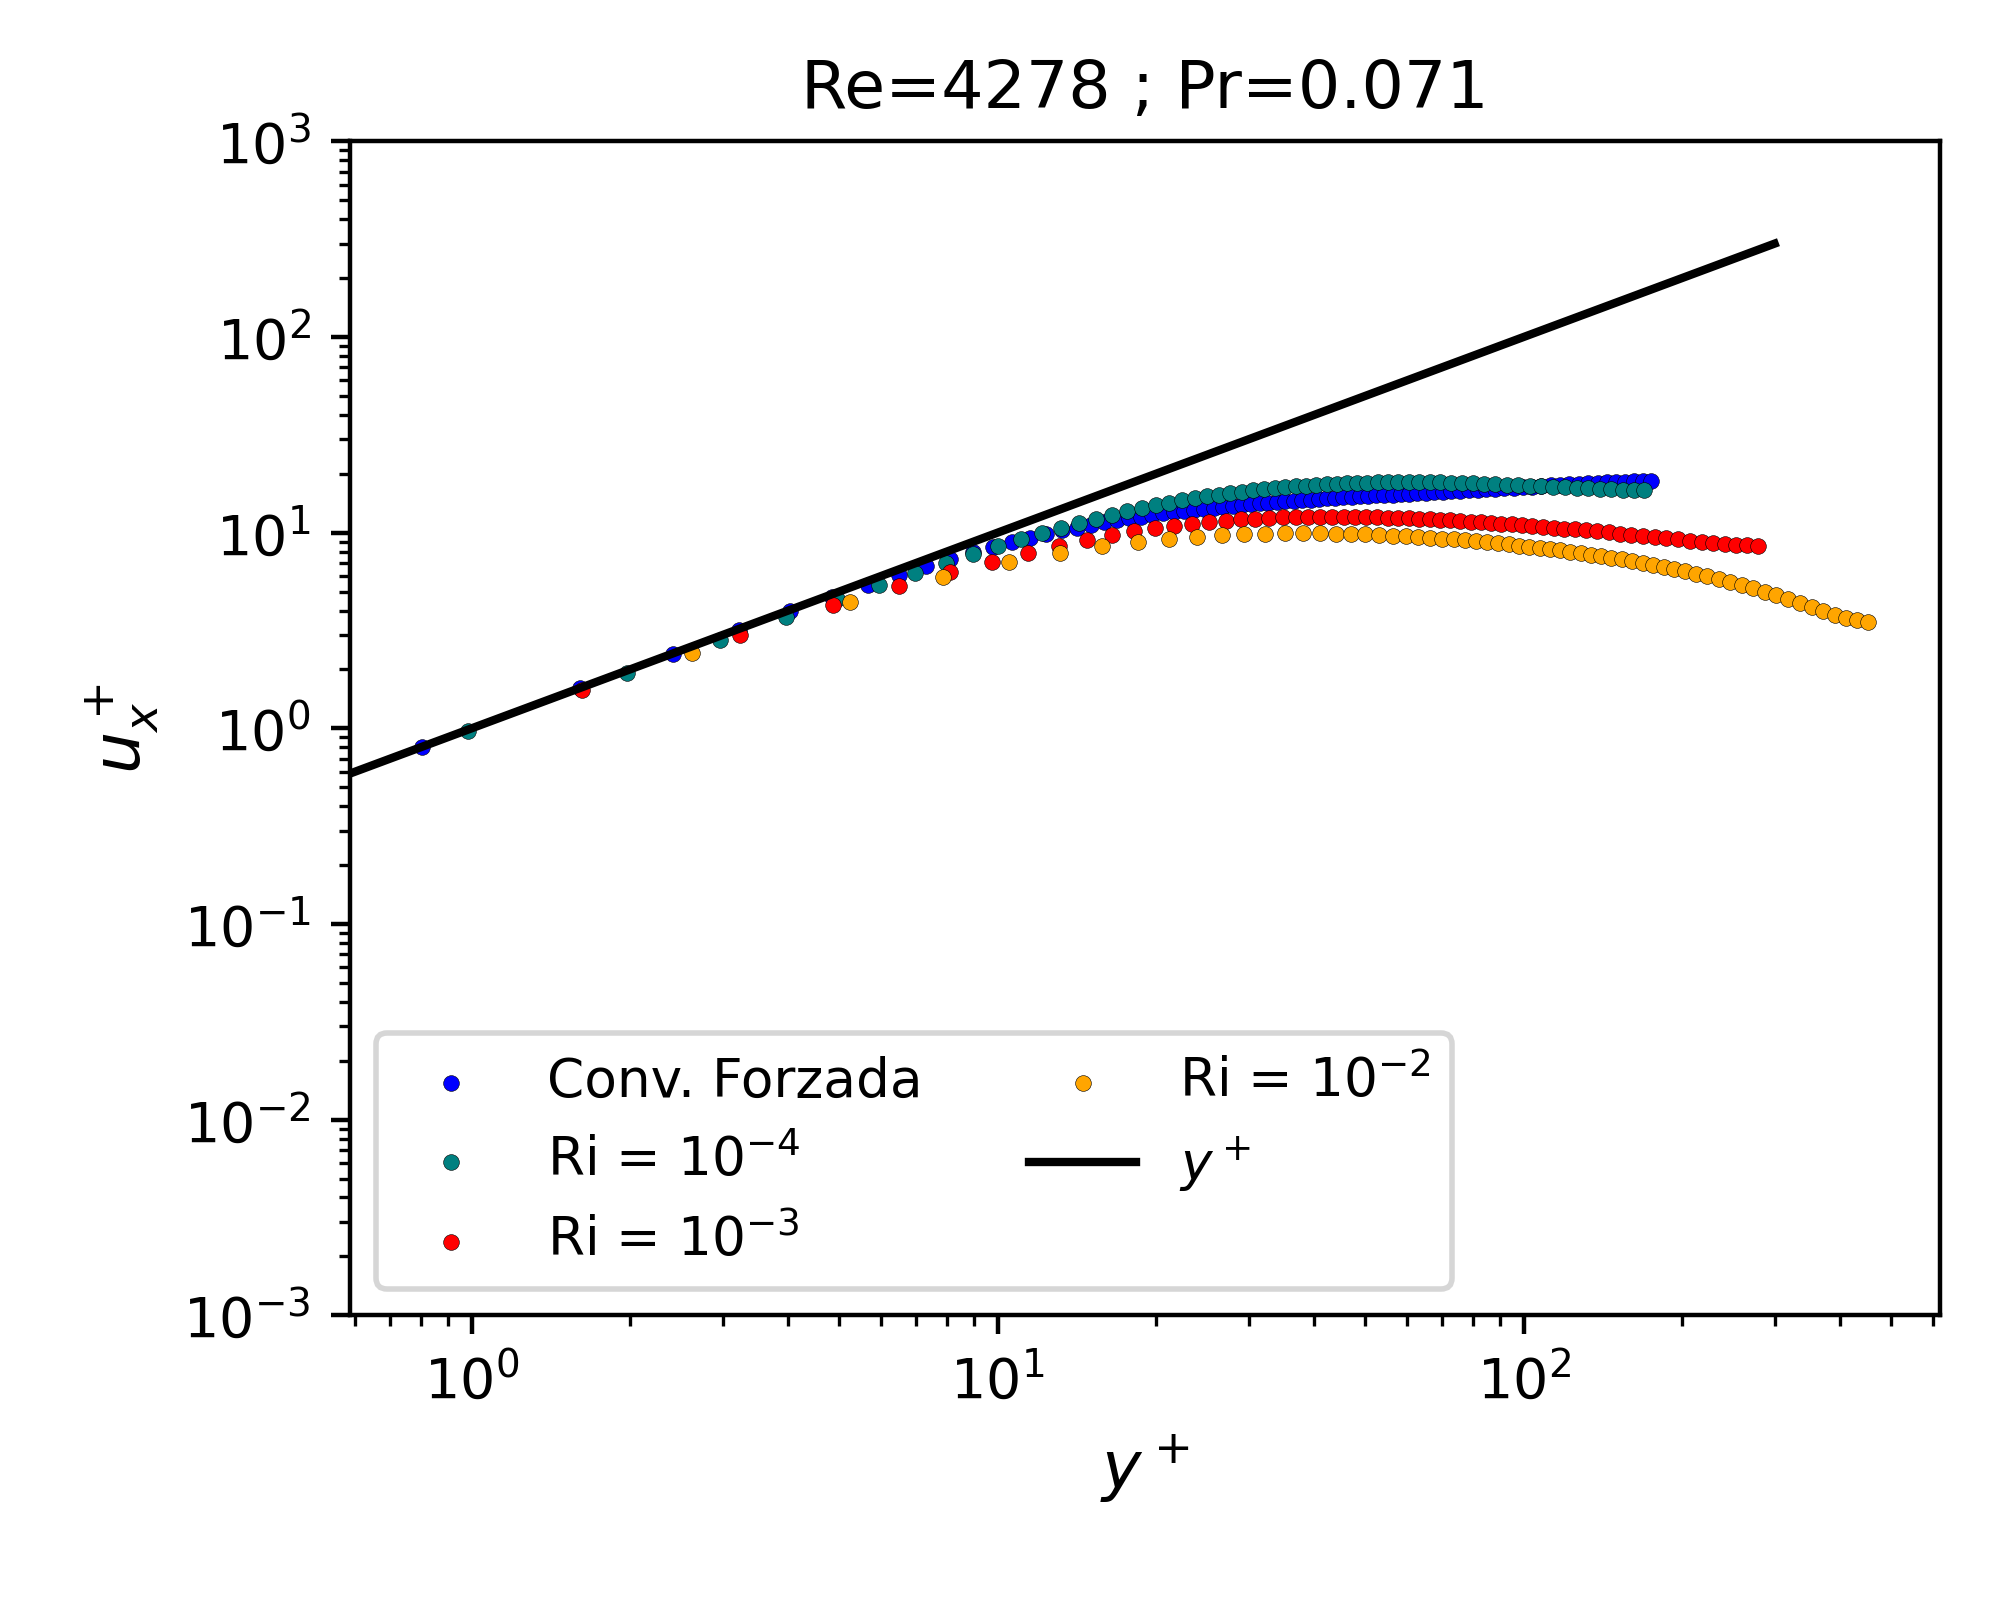
\includegraphics[width=0.45\textwidth]{figures/cap5/Re4278-Pr0071/ux_mean_plus_log_profile.png}}
  \subfloat[]{
    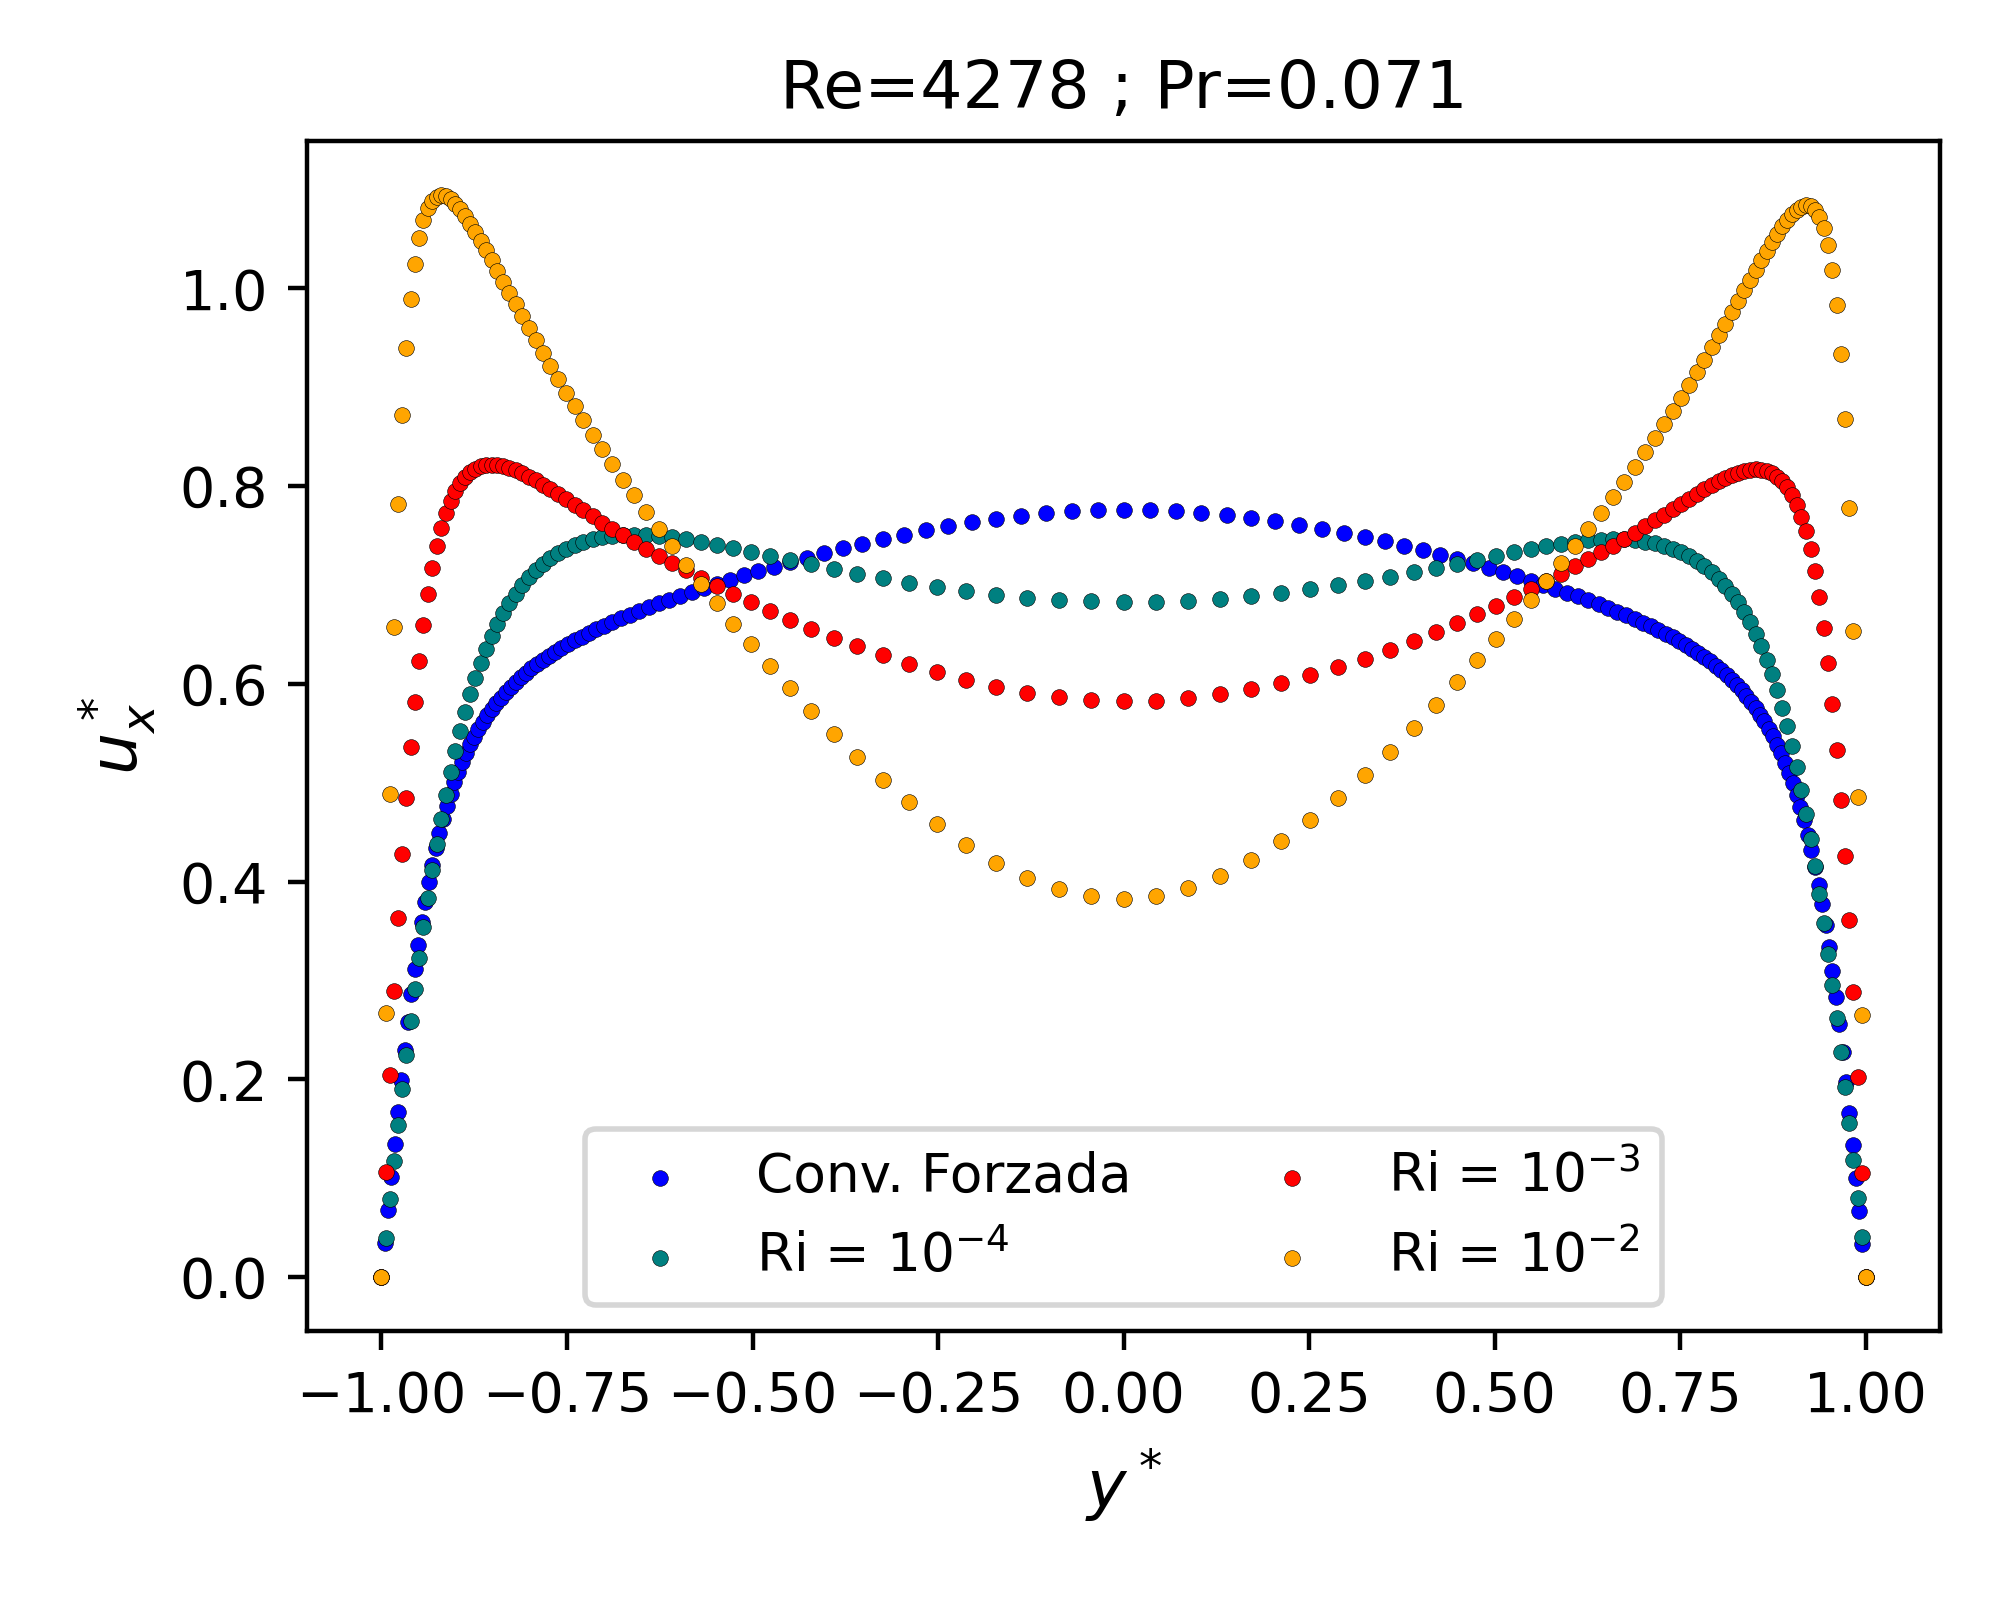
\includegraphics[width=0.45\textwidth]{figures/cap5/Re4278-Pr0071/ux_mean_profile.png}}
  \caption{}
  \label{fig:ux-Re4278-Pr0071}
\end{figure}

%% ==============================================================
%%  Re = 5000, Pr = 0.71
%% ==============================================================

\section{$\text{Re}=5000$ y $\text{Pr}=0.71$}

\begin{figure}[H]
  \centering
  \subfloat[]{
    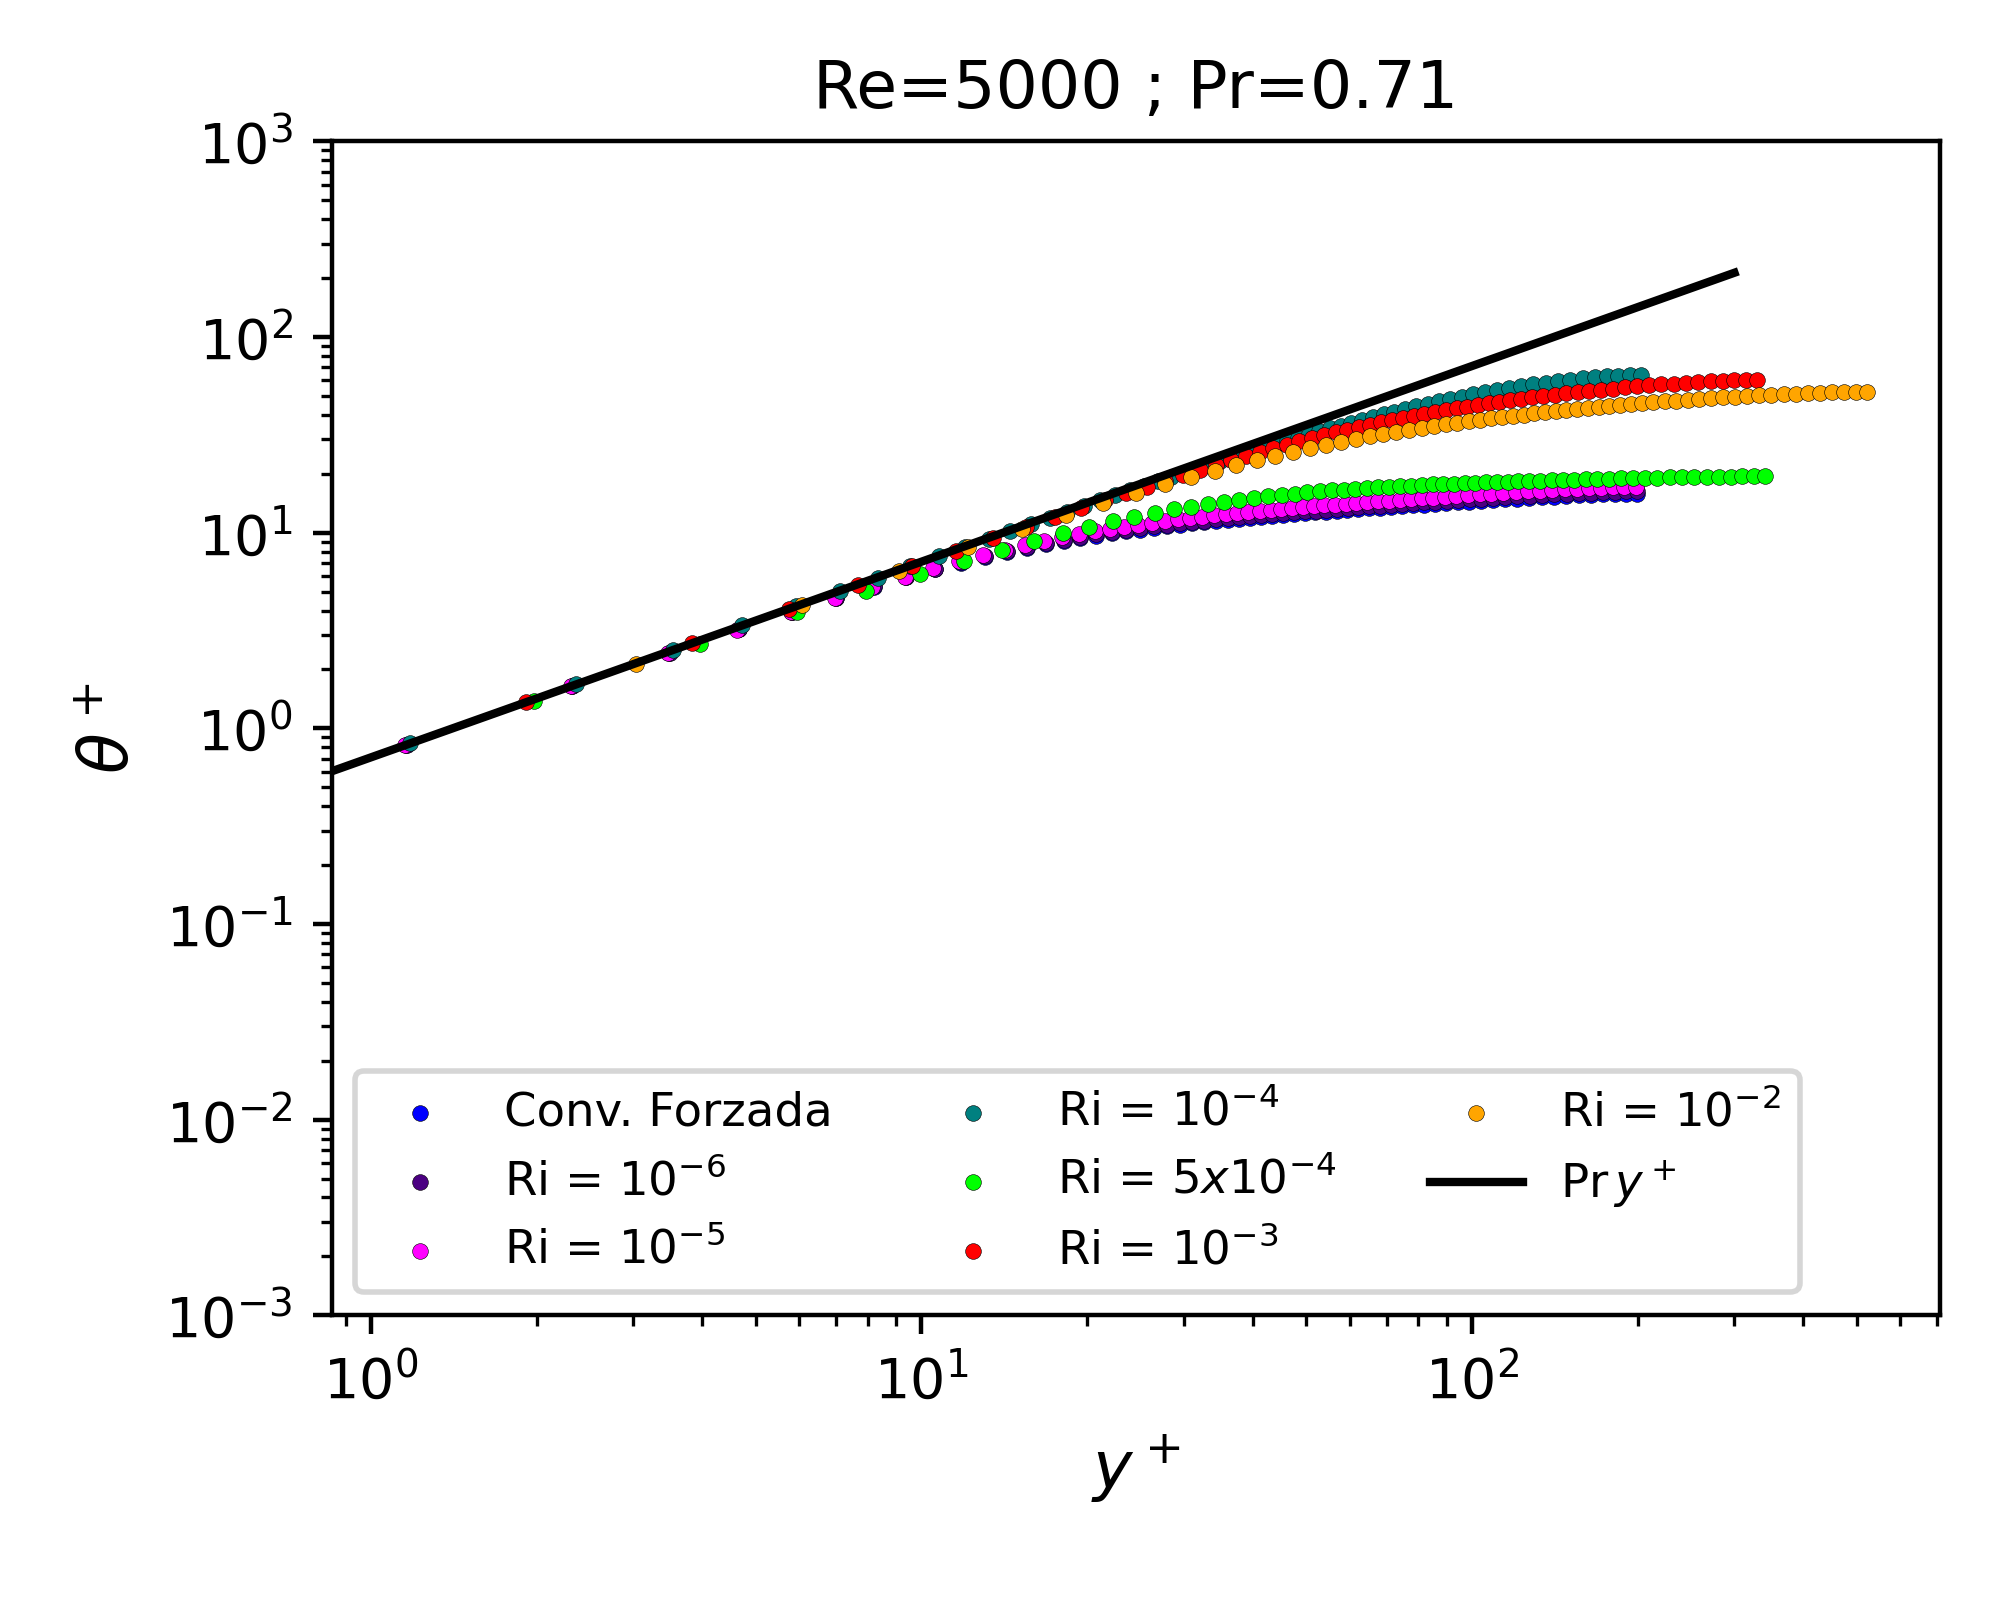
\includegraphics[width=0.45\textwidth]{figures/cap5/Re5000-Pr071/phi_mean_plus_log_profile.png}}
  \subfloat[]{
    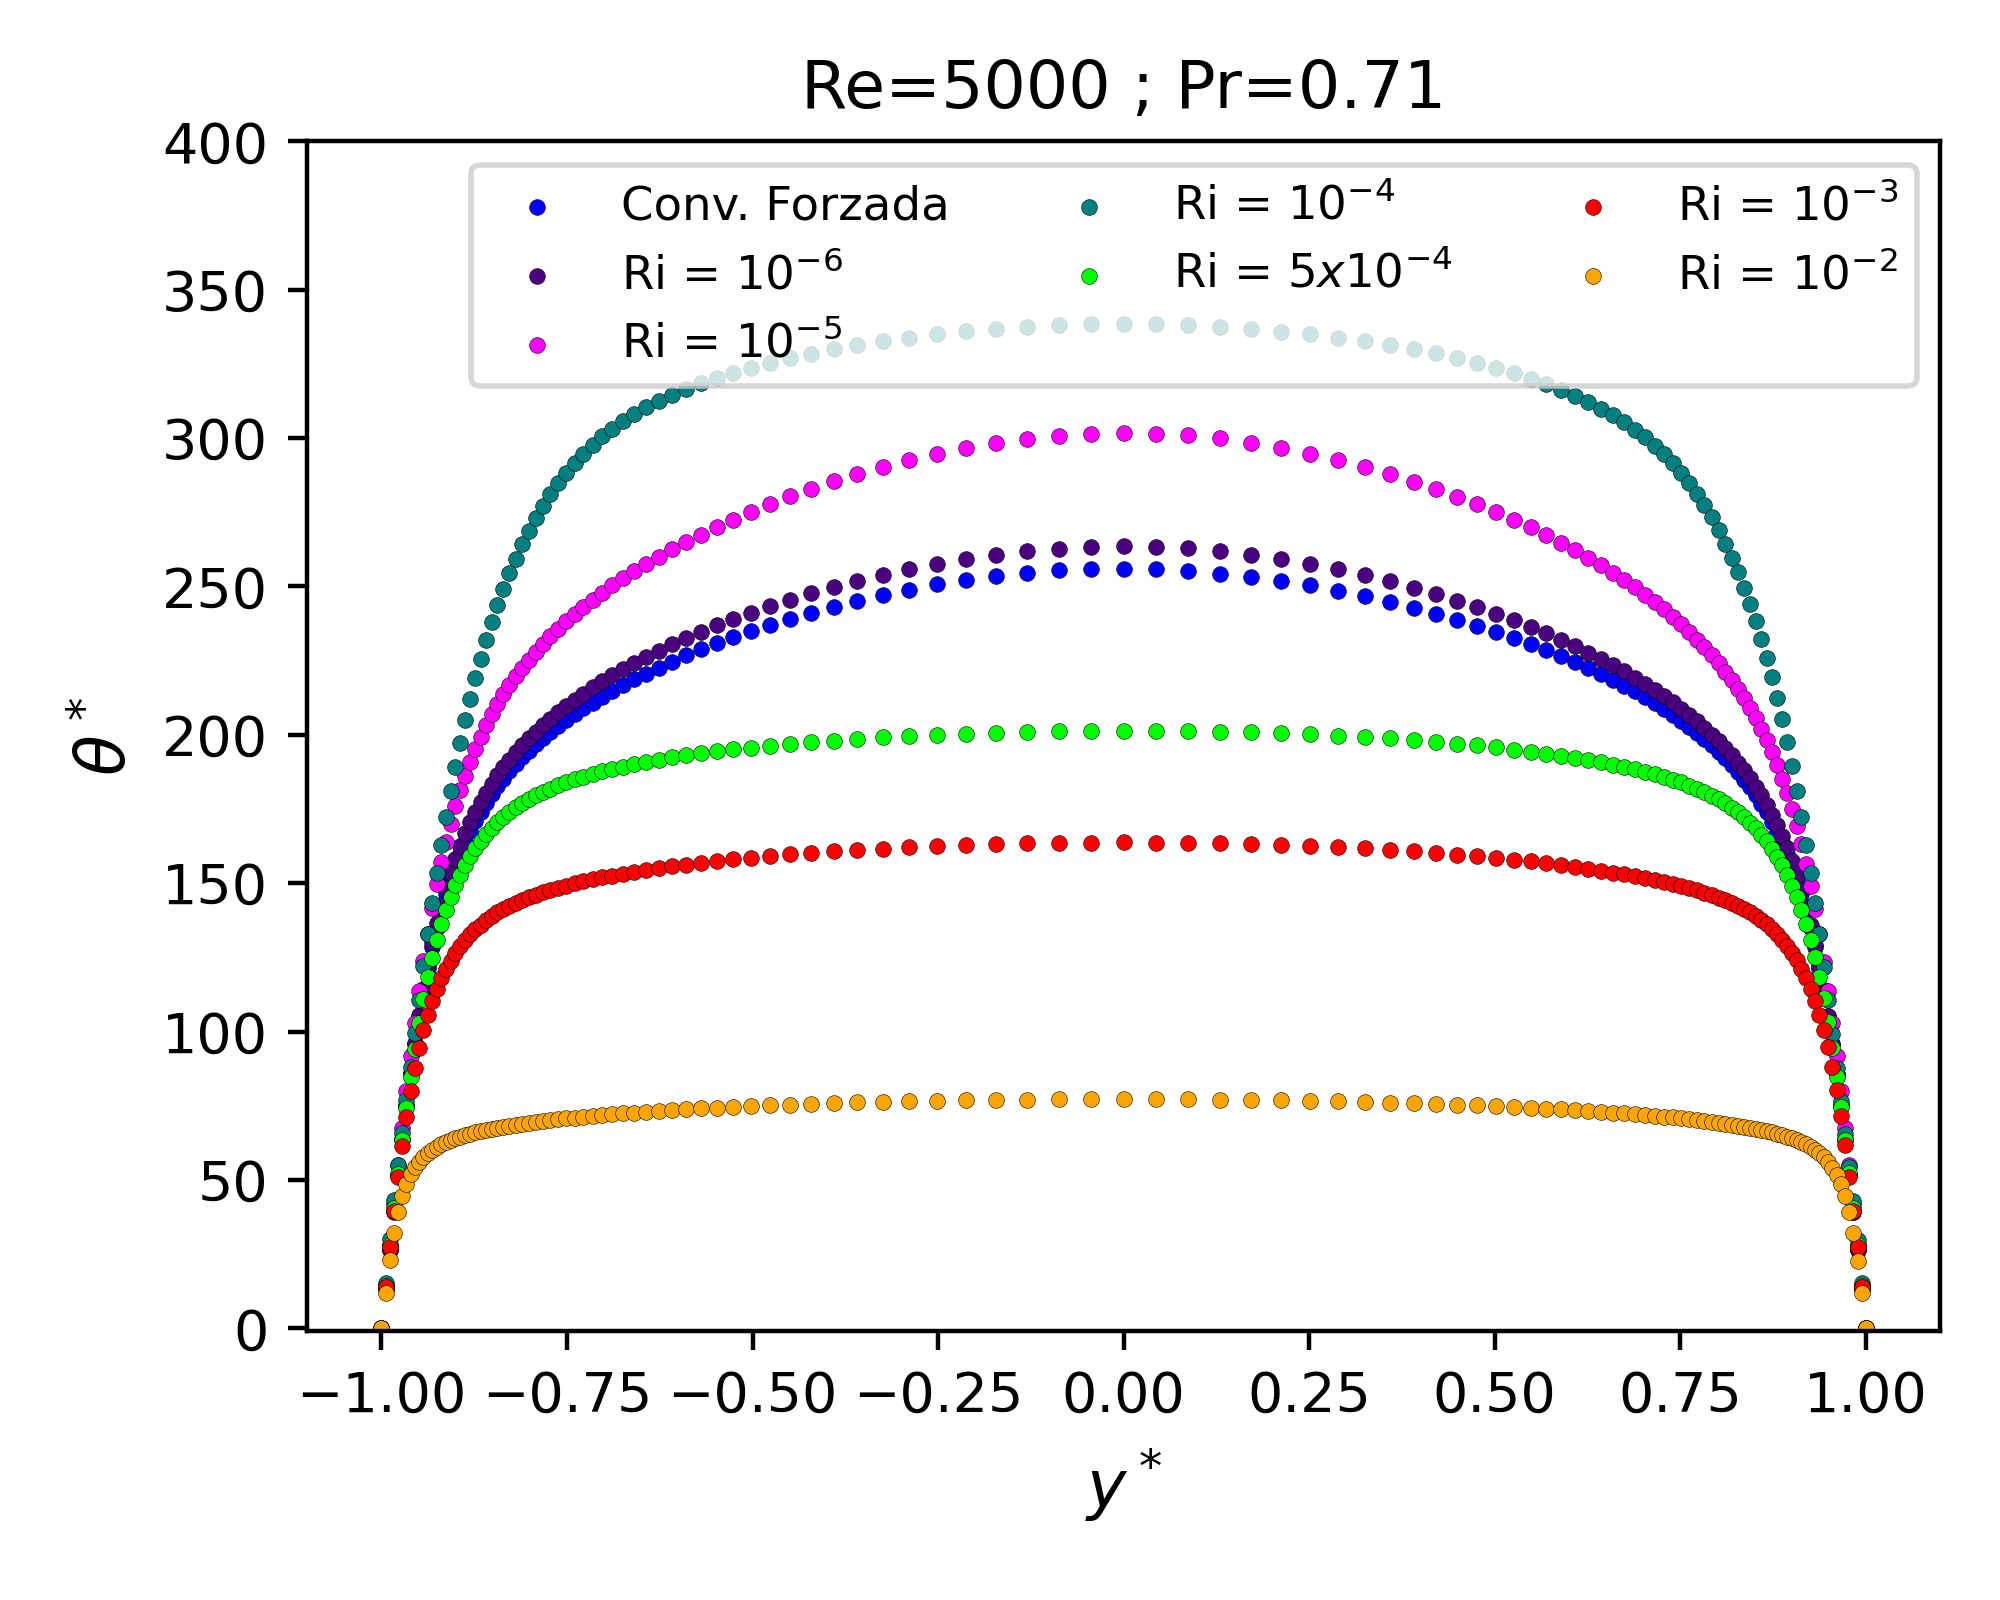
\includegraphics[width=0.45\textwidth]{figures/cap5/Re5000-Pr071/phi_mean_profile.png}}
  \caption{}
  \label{fig:phi-Re5000-Pr071}
\end{figure}

\begin{figure}[H]
  \centering
  \subfloat[]{
    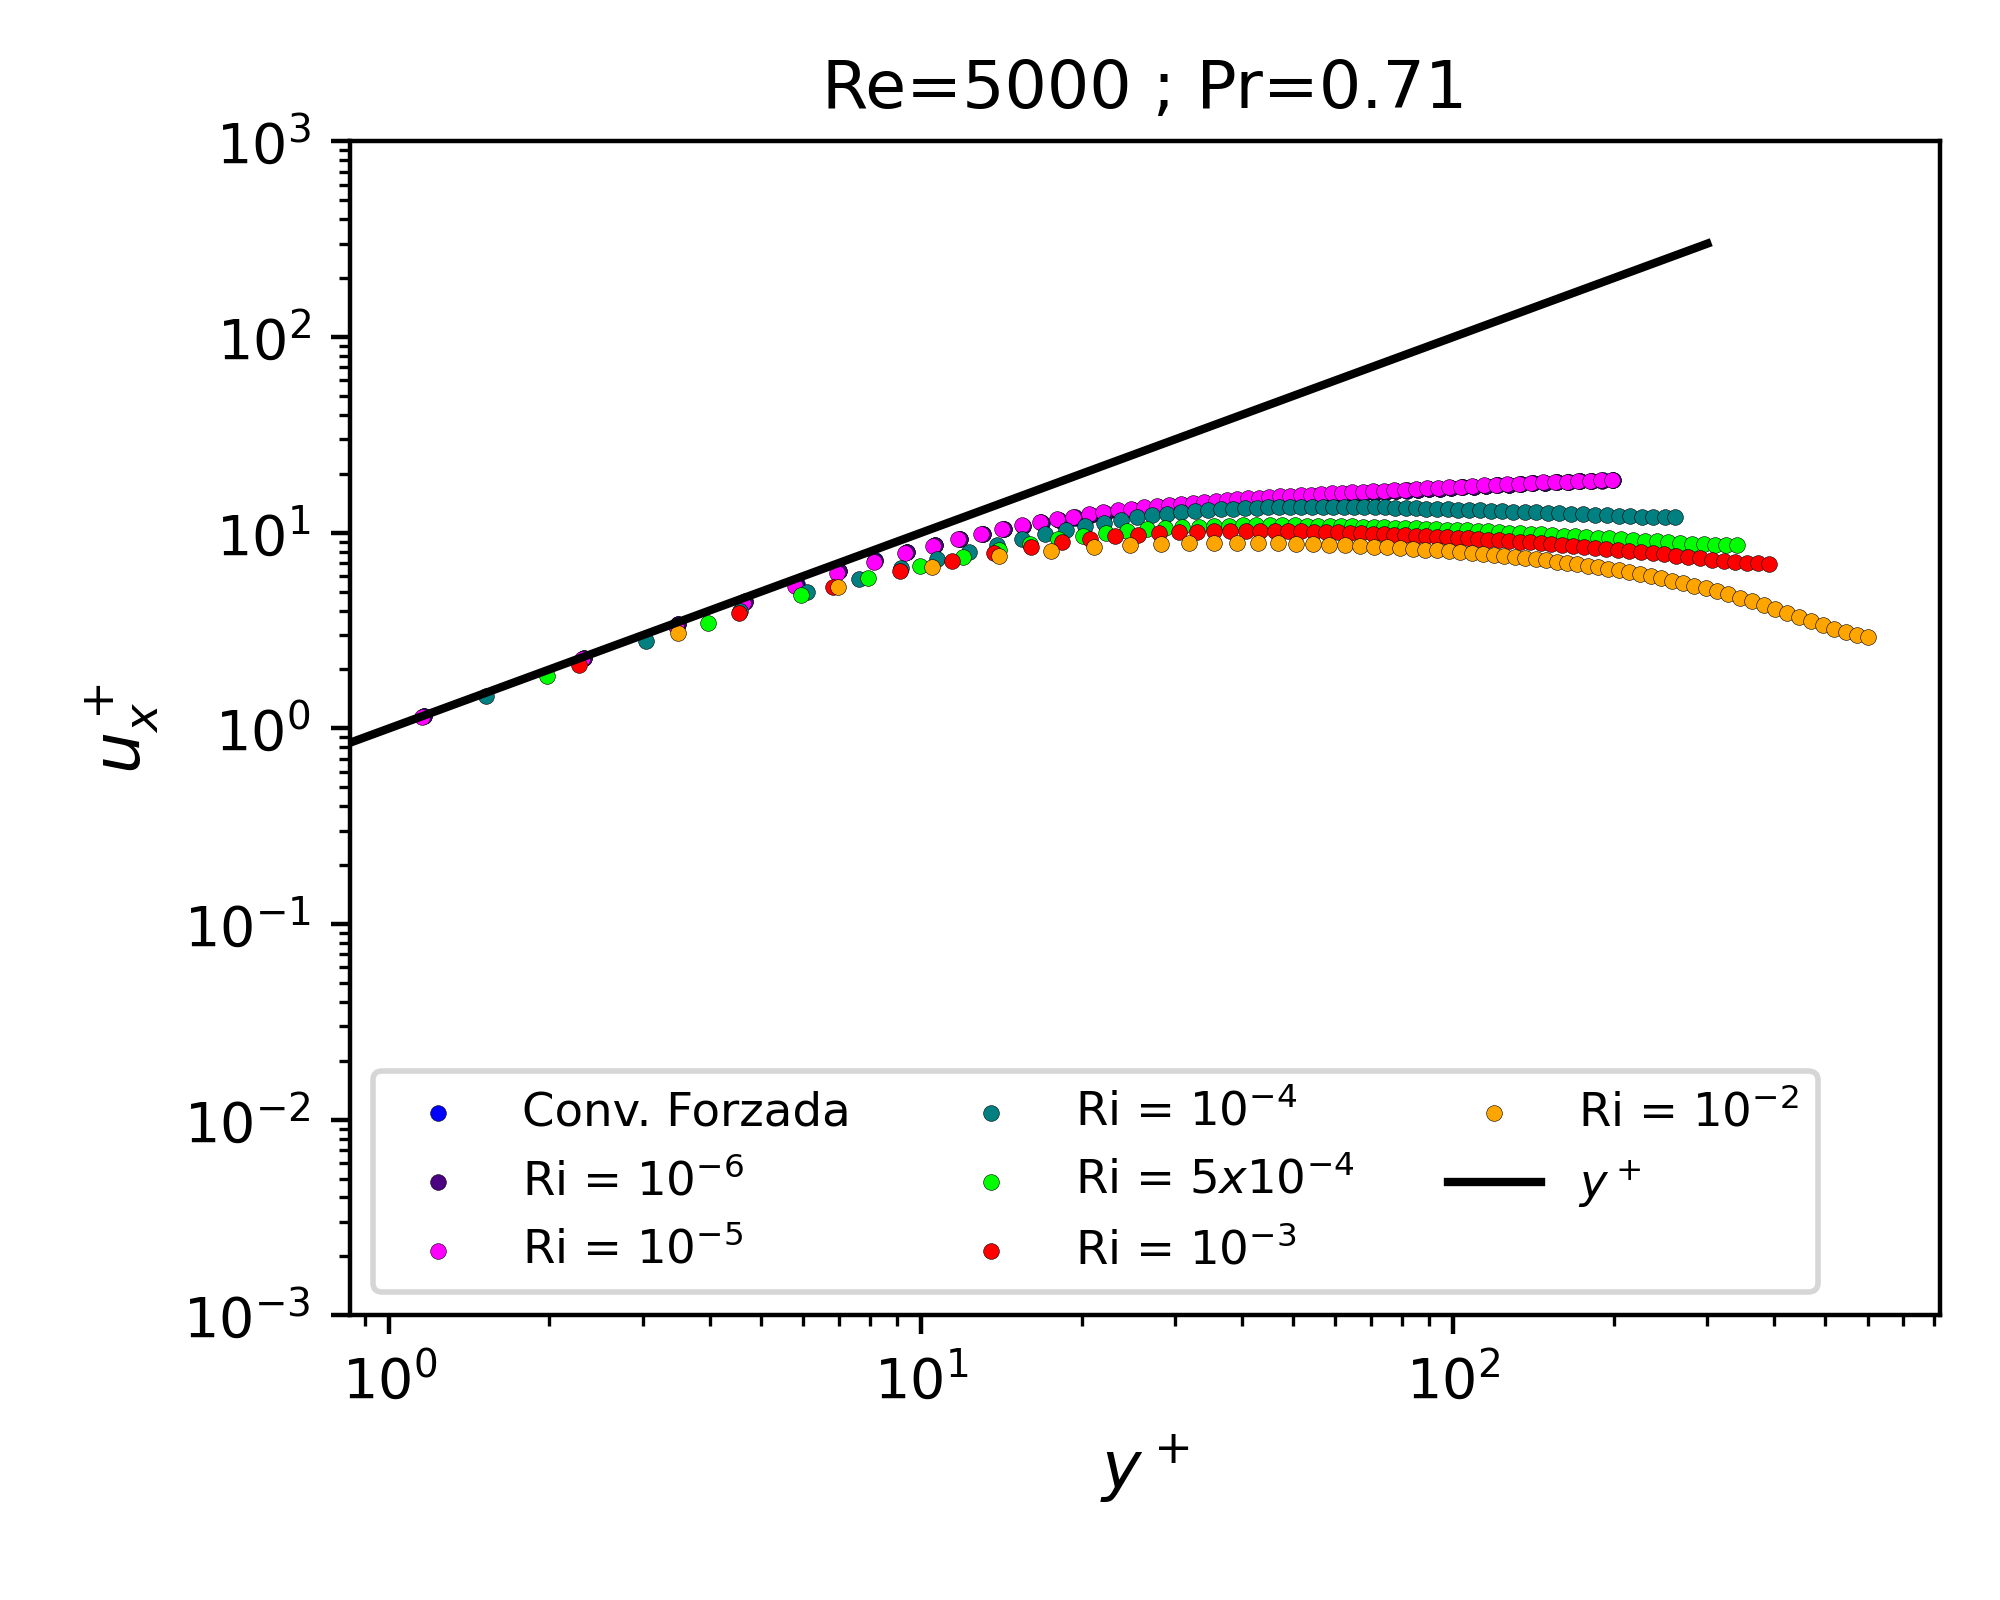
\includegraphics[width=0.45\textwidth]{figures/cap5/Re5000-Pr071/ux_mean_plus_log_profile.png}}
  \subfloat[]{
    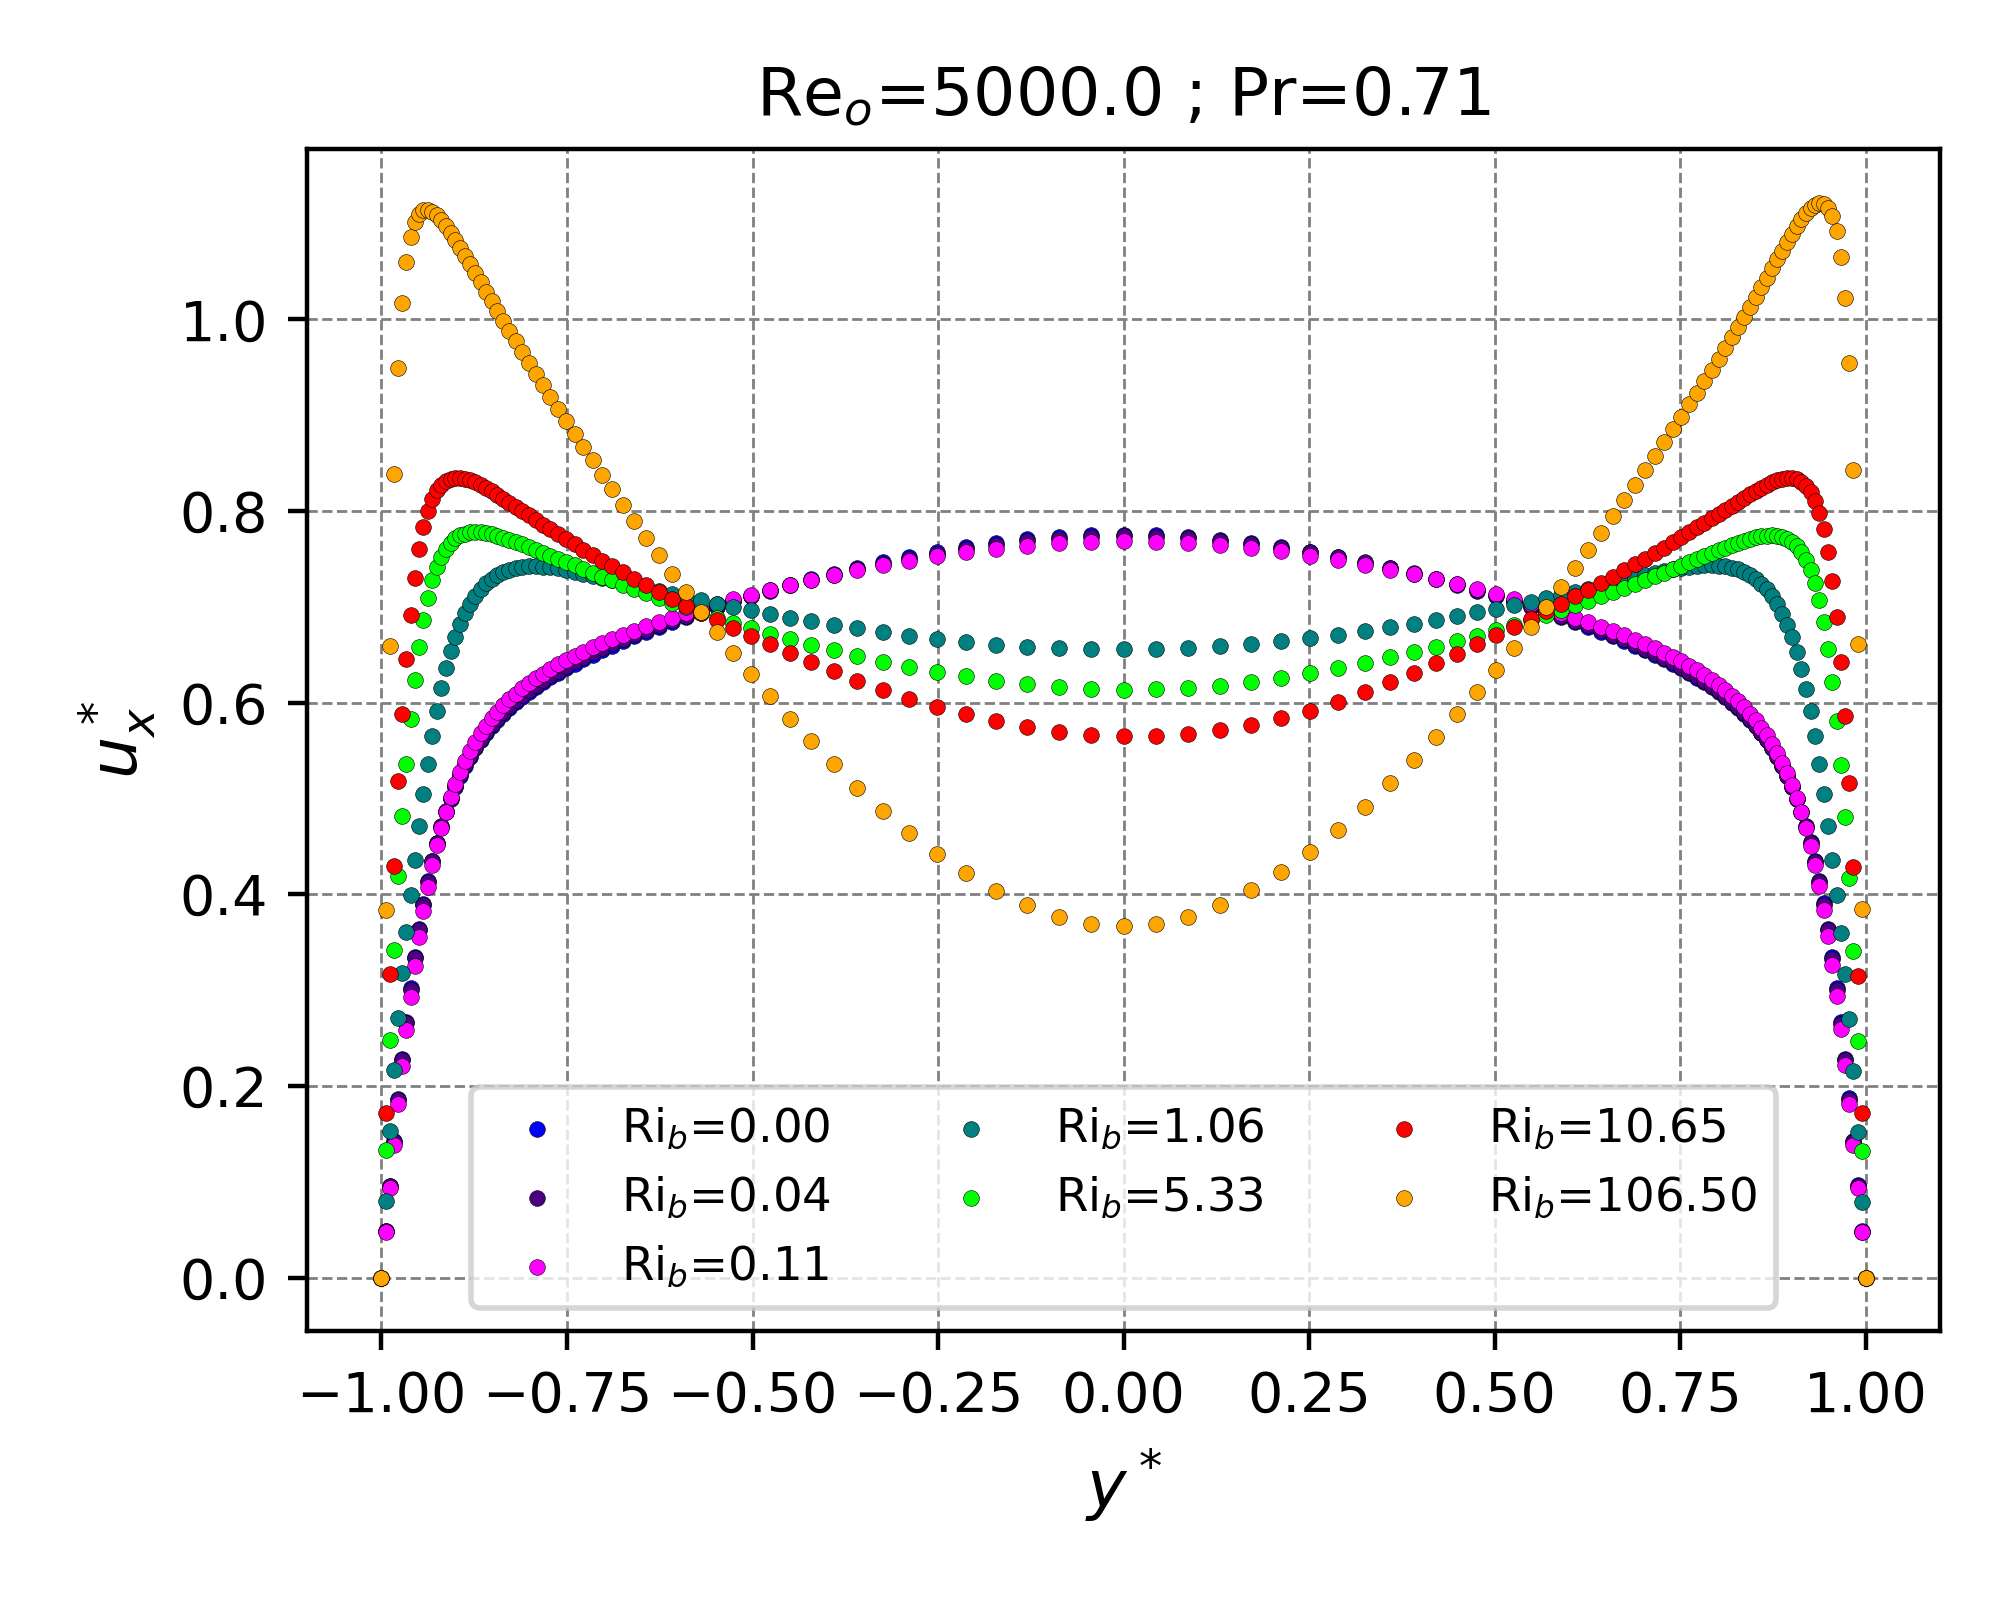
\includegraphics[width=0.45\textwidth]{figures/cap5/Re5000-Pr071/ux_mean_profile.png}}
  \caption{}
  \label{fig:ux-Re5000-Pr071}
\end{figure}

%% ==============================================================
%%  Re = 5000, Pr = 0.071
%% ==============================================================

\section{$\text{Re}=5000$ y $\text{Pr}=0.071$}

\begin{figure}[H]
  \centering
  \subfloat[]{
    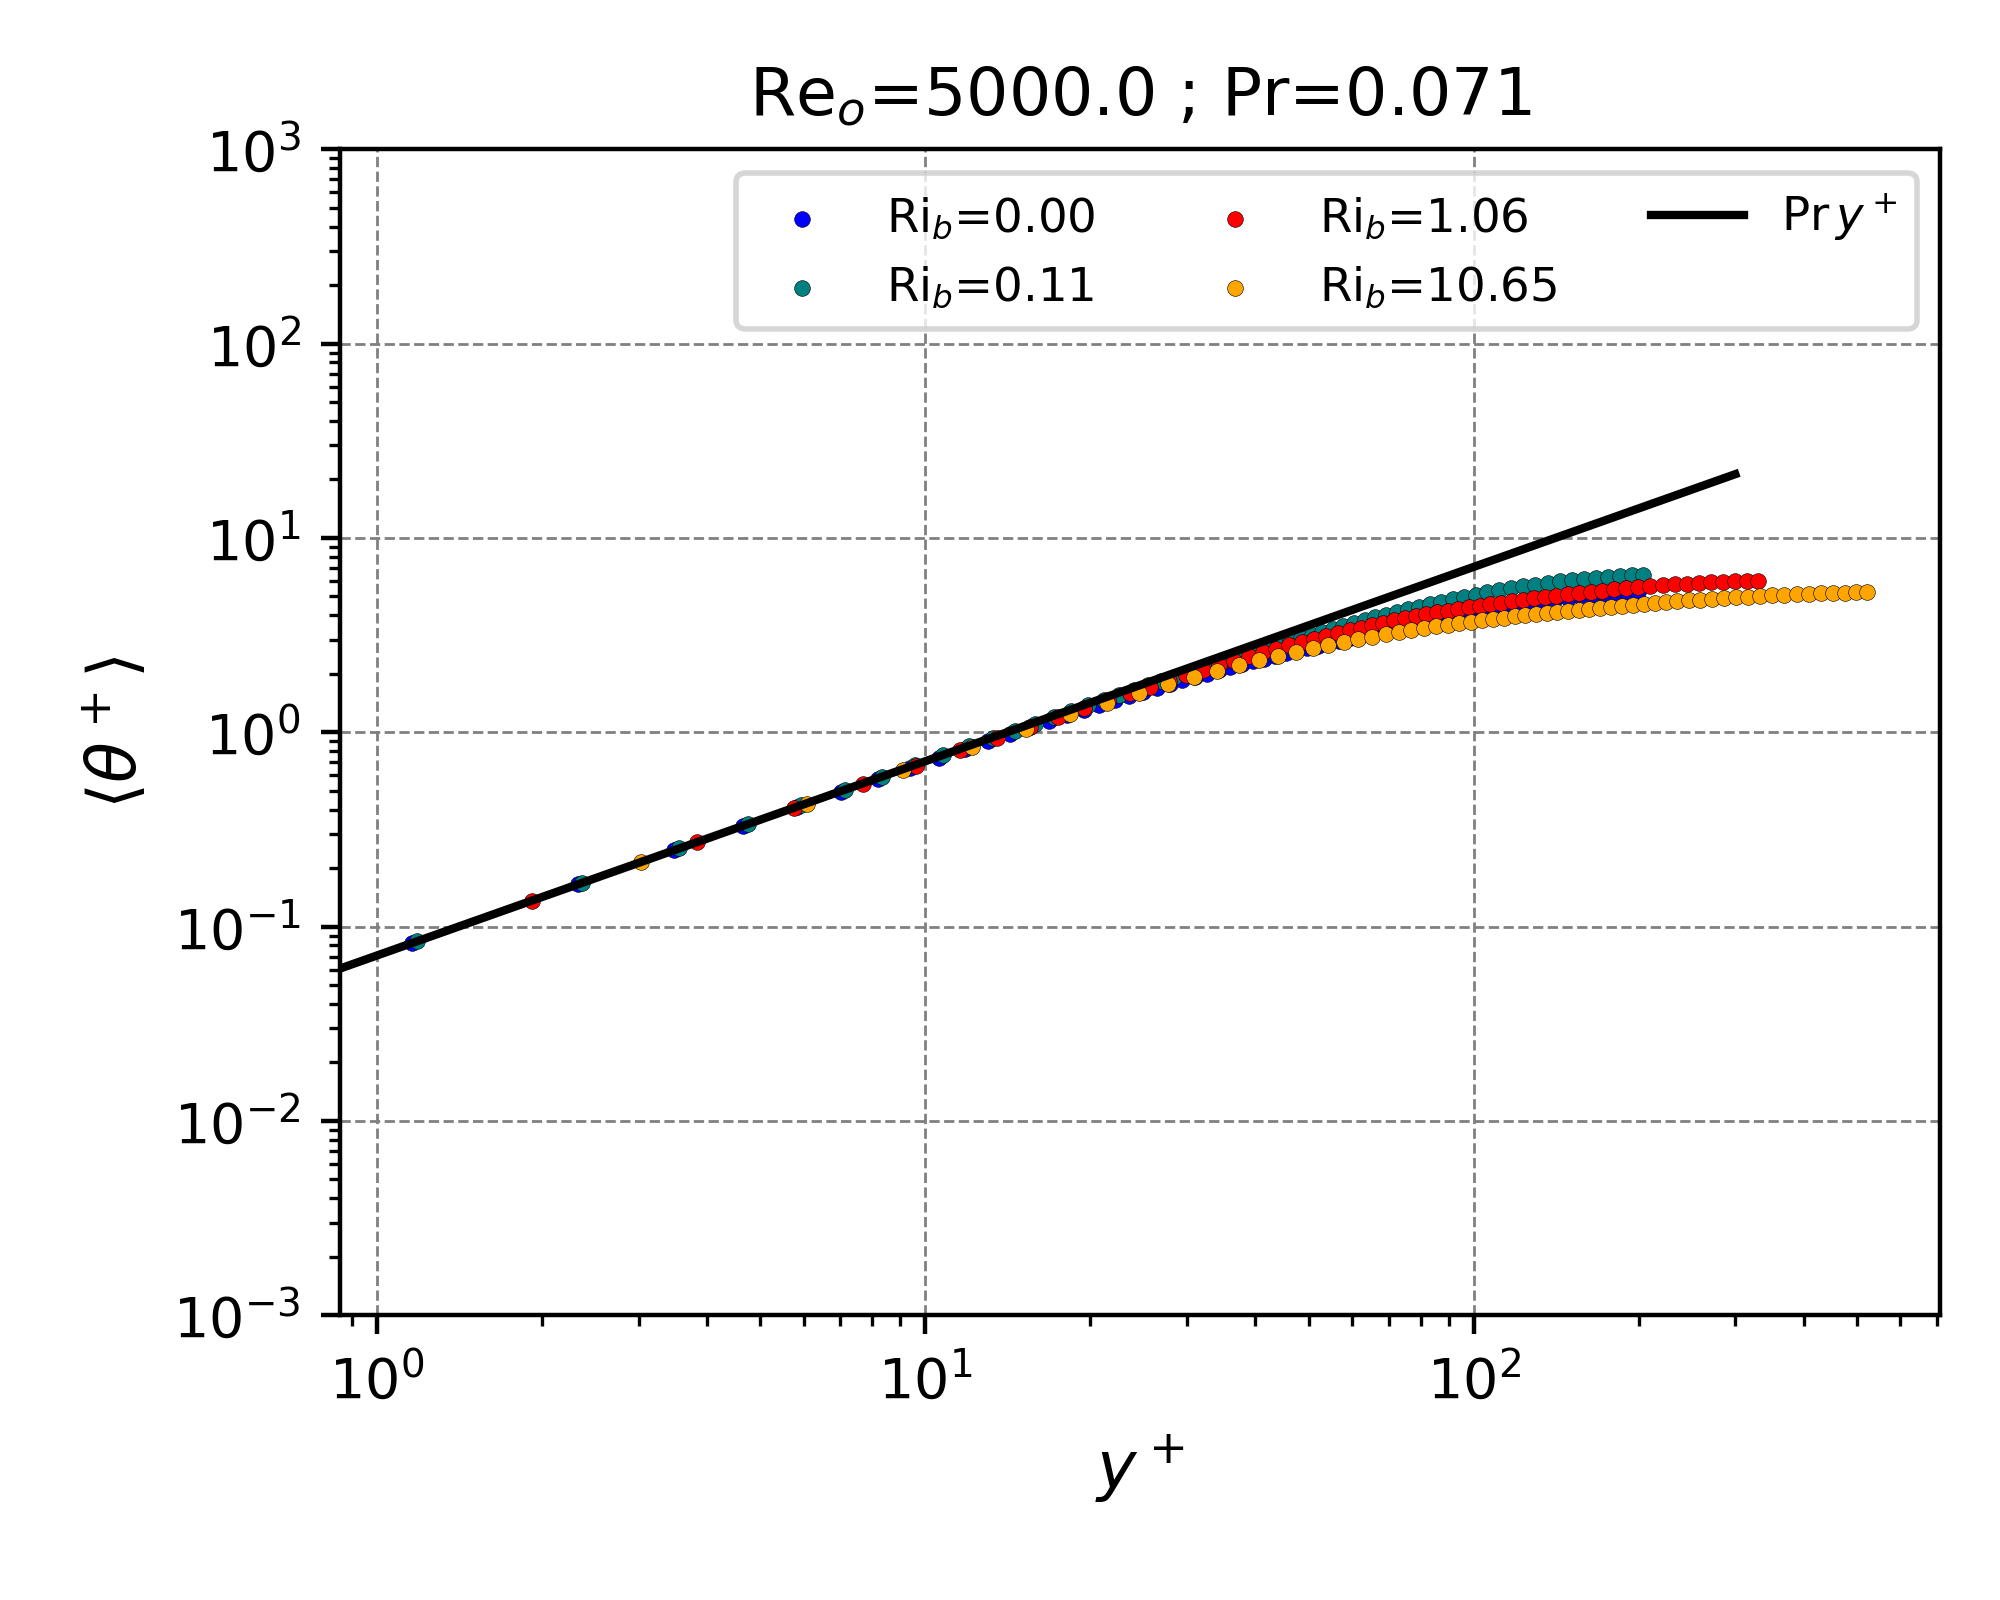
\includegraphics[width=0.45\textwidth]{figures/cap5/Re5000-Pr0071/phi_mean_plus_log_profile.png}}
  \subfloat[]{
    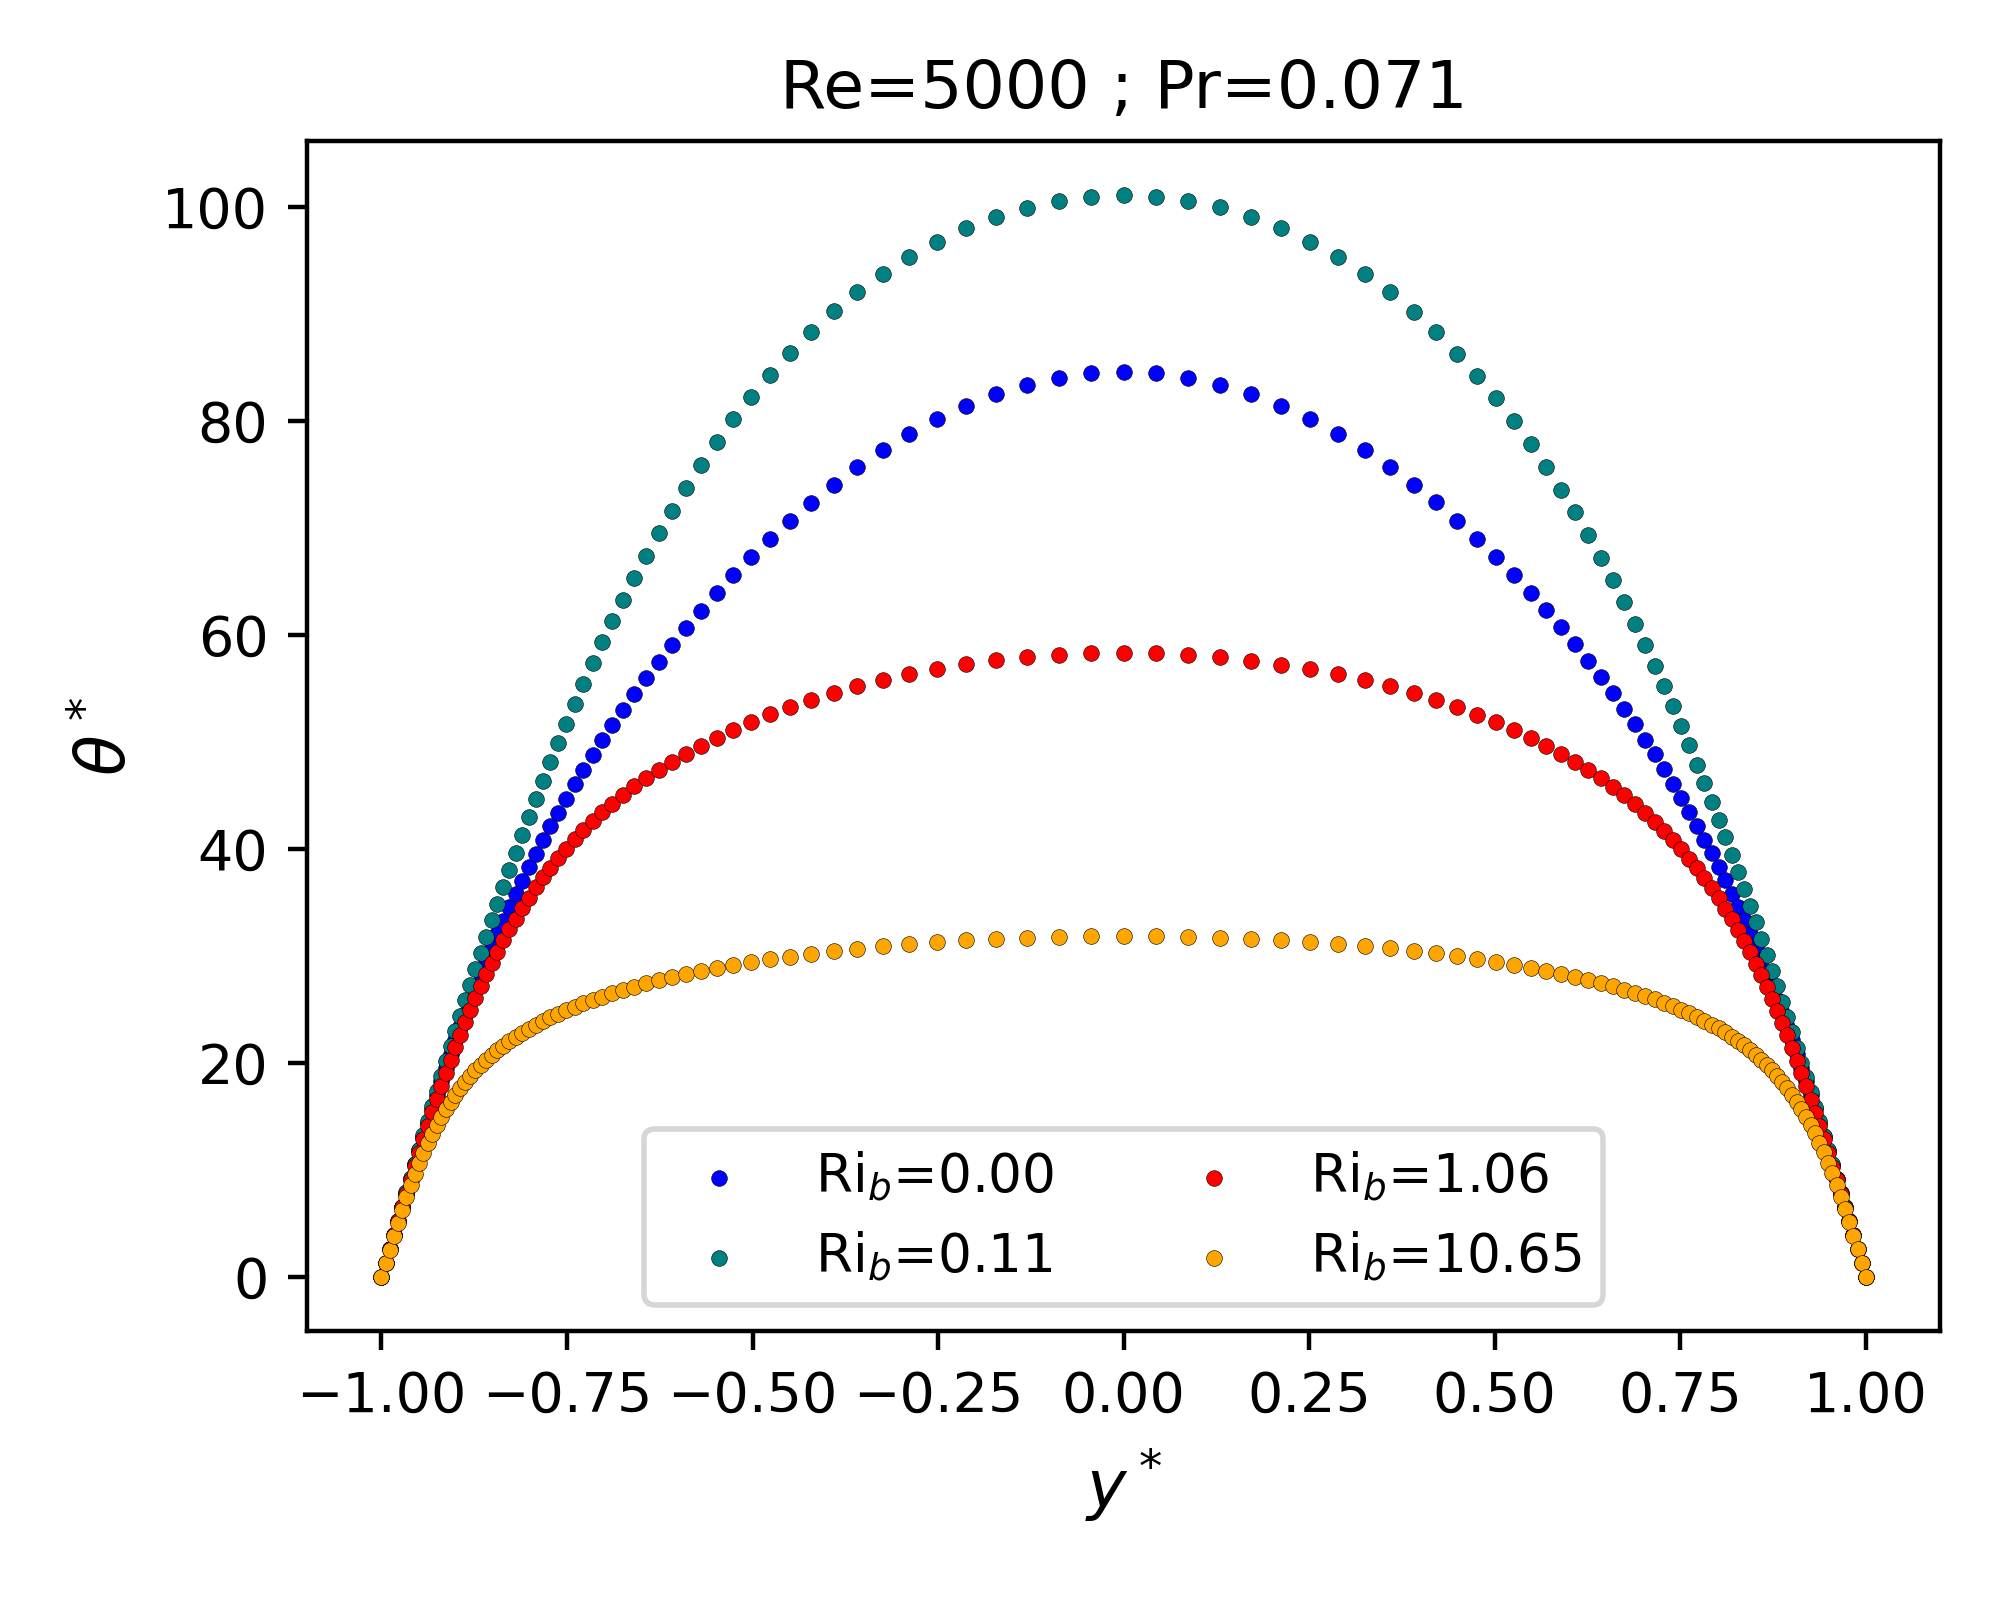
\includegraphics[width=0.45\textwidth]{figures/cap5/Re5000-Pr0071/phi_mean_profile.png}}
  \caption{}
  \label{fig:phi-Re5000-Pr0071}
\end{figure}

\begin{figure}[H]
  \centering
  \subfloat[]{
    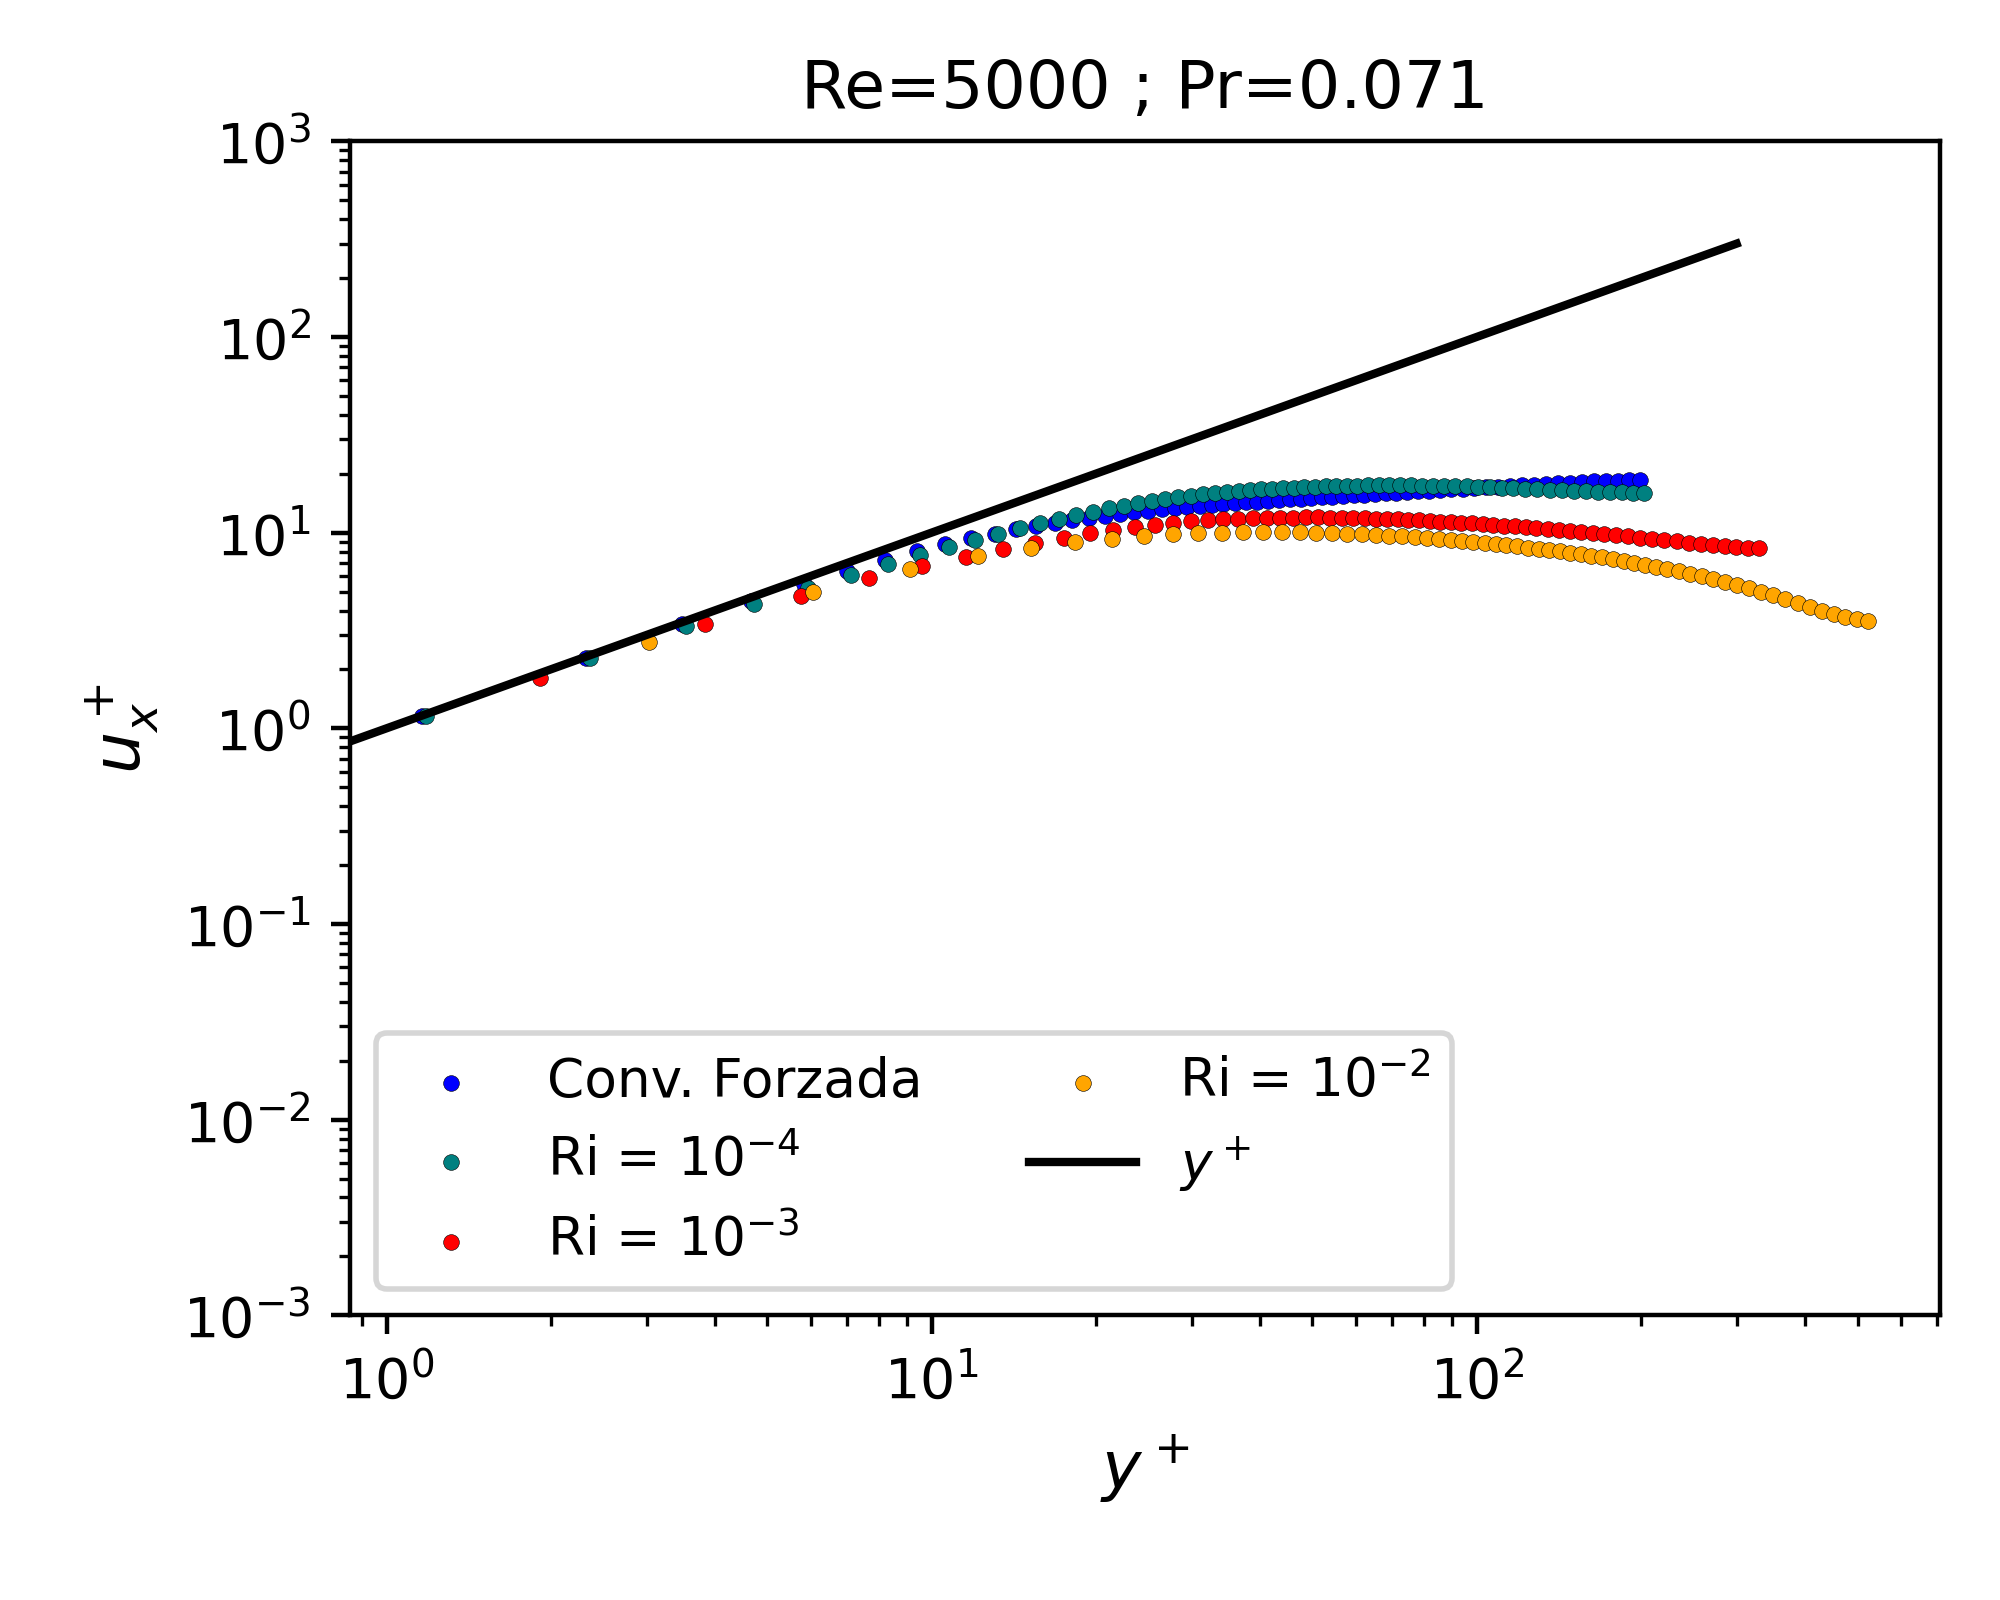
\includegraphics[width=0.45\textwidth]{figures/cap5/Re5000-Pr0071/ux_mean_plus_log_profile.png}}
  \subfloat[]{
    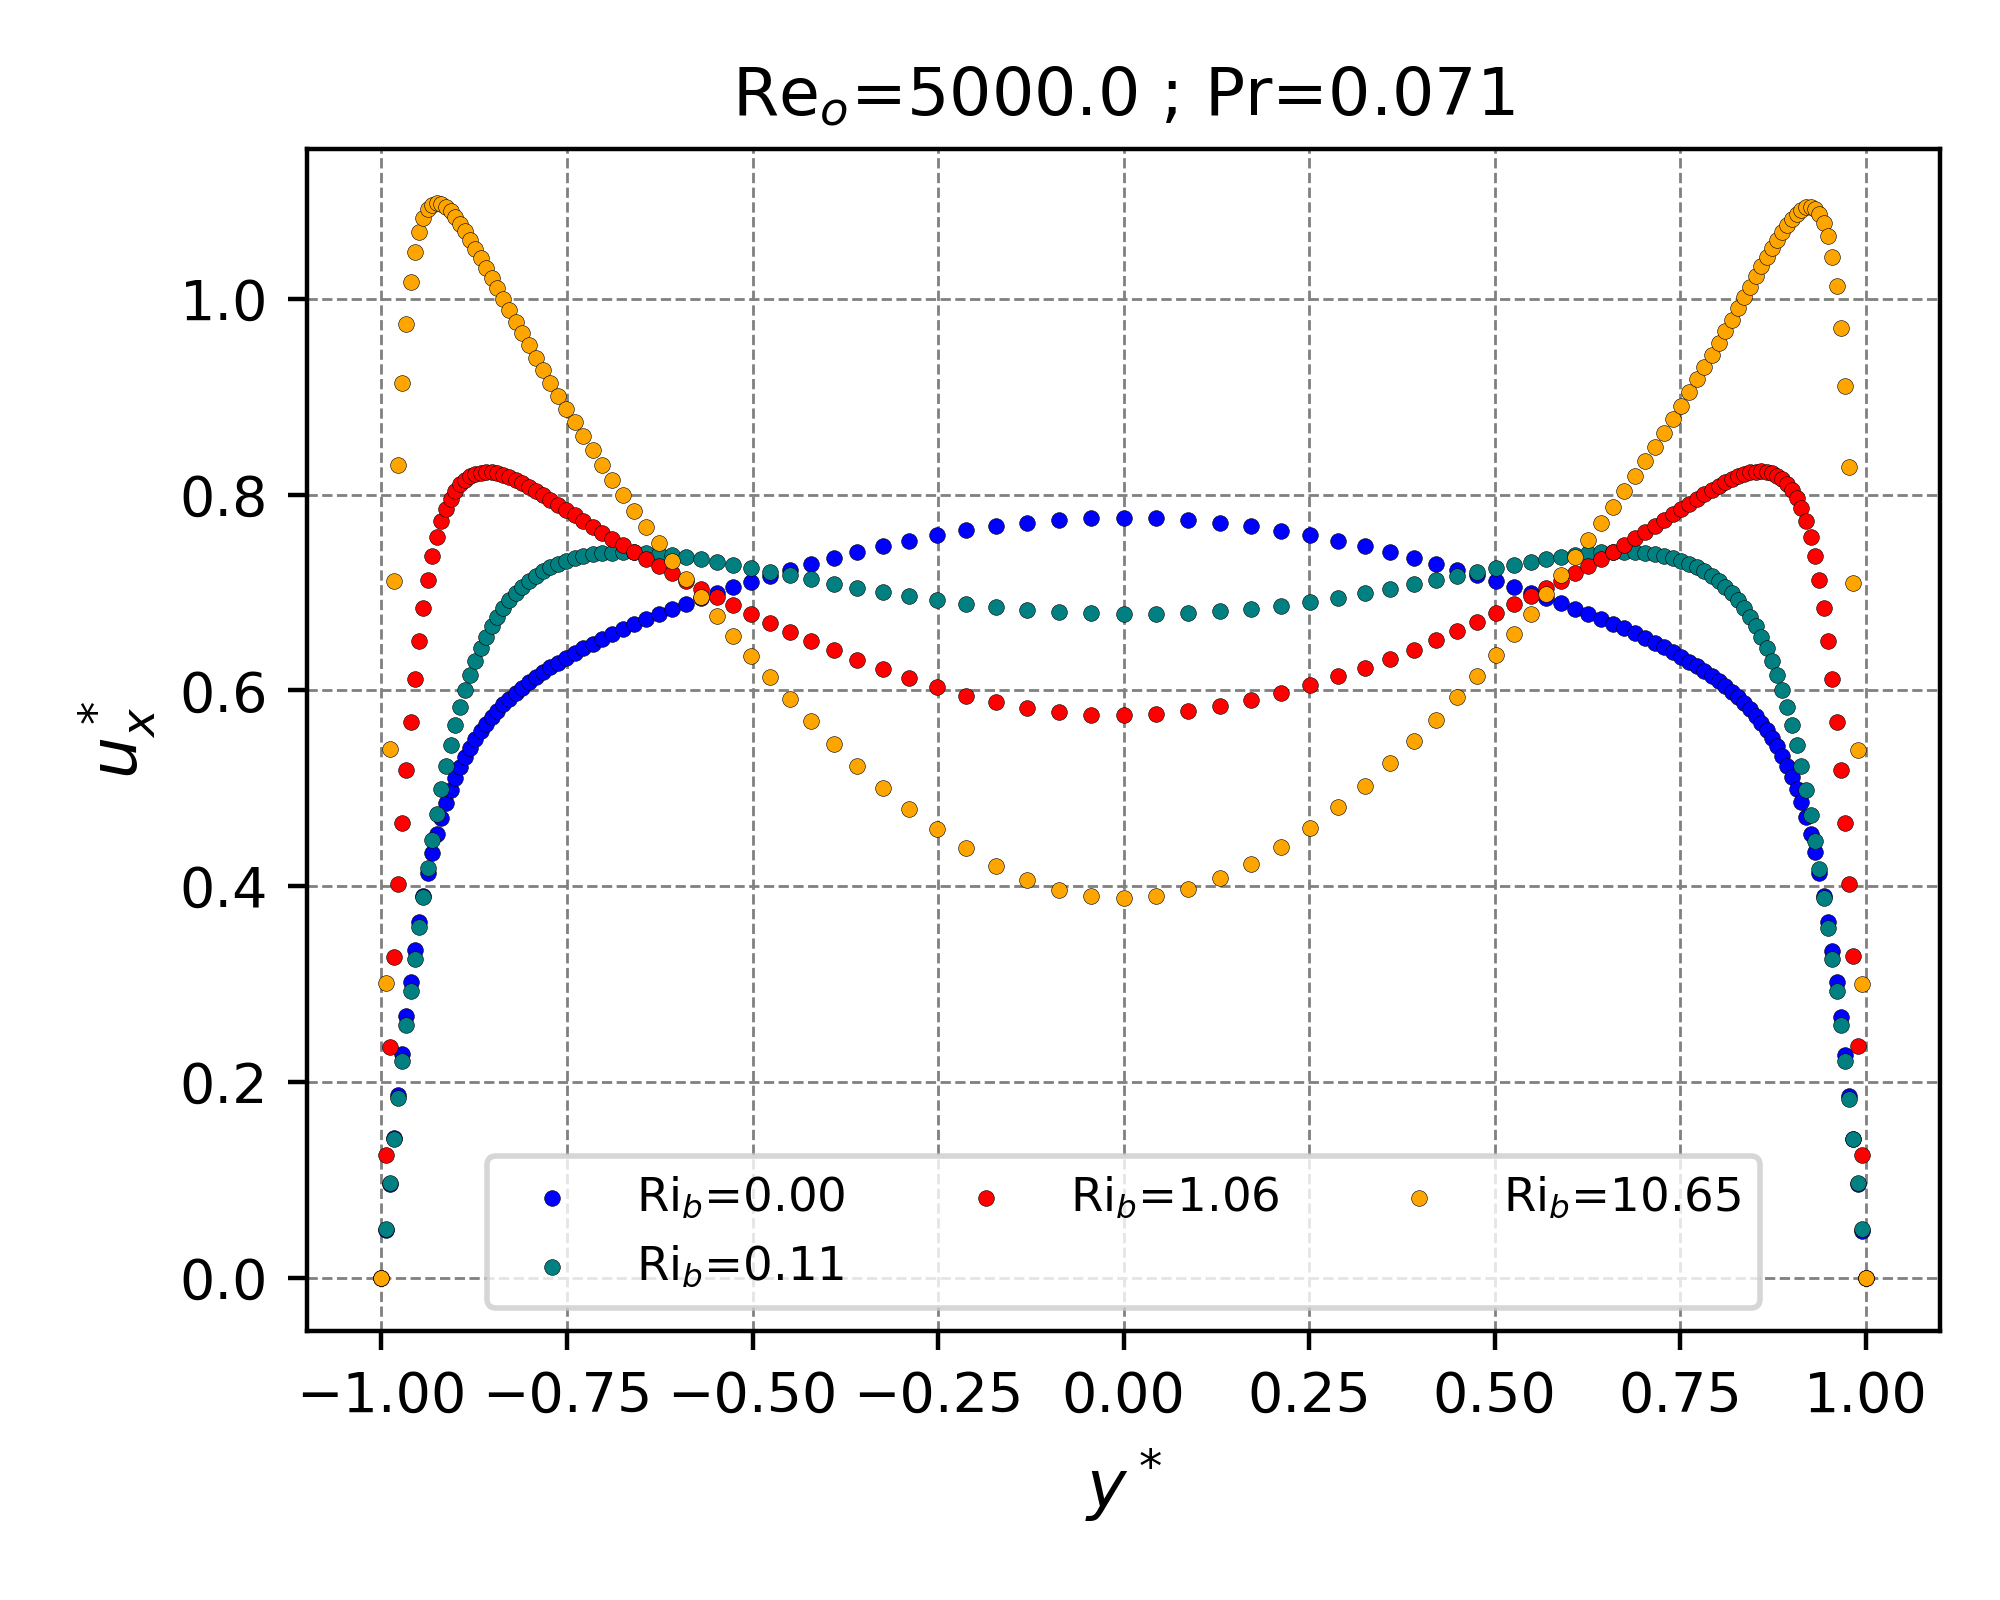
\includegraphics[width=0.45\textwidth]{figures/cap5/Re5000-Pr0071/ux_mean_profile.png}}
  \caption{}
  \label{fig:ux-Re5000-Pr0071}
\end{figure}


Faltan graficas de correlaciones (Nu, Re$_{\tau}$) vs Re y (Nu, Re$_{\tau}$) vs Ri.

Adicionalmente tengo simulaciones con Re=2100 ; Pr=1,0.1 ; Ri=10$^{-2}$,10$^{-3}$,10$^{-4}$ que no recuerdo porque las hice pero quizás podrian servir para la correlacion/análisis (Nu, Re$_{\tau}$) vs Ri del caso Re=2100.	